\documentclass[12pt]{article}

% load packages 
\usepackage{mathptmx}
\usepackage{amsmath}
\usepackage{geometry}
\usepackage{graphicx}
\usepackage{wrapfig}
\usepackage{afterpage}
\usepackage{natbib}
\usepackage{setspace}
\usepackage{abstract}
\usepackage{tocloft}
\usepackage[toc, page, title]{appendix}
\usepackage{multirow}
\usepackage{tabularx}
\usepackage{float}
\usepackage{caption}
\usepackage{subcaption}
\usepackage{indentfirst}
\usepackage{sectsty}
\usepackage{rotating}
\usepackage{pdflscape}

% page layout
\geometry{margin=0.8in}
\setstretch{1.5}
\setlength\parindent{20pt}\setlength{\parskip}{0.0pt plus 0.0pt}

% text formatting
\sectionfont{\large \scshape}
\subsectionfont{\normalsize}
\subsubsectionfont{\normalsize\itshape}
\setcounter{secnumdepth}{4}
\renewcommand{\abstractname}{Résumé}
\setlength{\abstitleskip}{-0.5em}
\renewcommand{\abstractnamefont}{\normalfont \large \bfseries \scshape}
\renewcommand{\abstracttextfont}{\normalfont \normalsize}
\renewcommand\refname{Bibliographie}
\renewcommand{\tablename}{Tableau}
\renewcommand{\contentsname}{Sommaire}
\renewcommand{\appendixtocname}{Annexes}
\renewcommand{\appendixpagename}{\large \scshape \bfseries Annexes}
\renewcommand{\appendixname}{Annexe}
\renewcommand{\setthesection}{\Alph{section}}


% toc formatting
\setlength\cftsecindent{0pt}
\setlength\cftsubsecindent{20pt}
\setlength\cftsubsubsecindent{48pt}
\setlength\cftbeforesecskip{18pt}
\setlength\cftbeforesubsecskip{10pt}
\setlength\cftbeforesubsubsecskip{8pt}
\renewcommand{\cftsubsecfont}{ }
\renewcommand{\cftsubsubsecfont}{ }
\renewcommand{\cftdot}{.}
\renewcommand{\cfttoctitlefont}{\large \scshape \bfseries}
\renewcommand{\cftpnumalign}{l}
\setlength{\cftbeforefigskip}{5pt}
\cftsetpnumwidth{50pt}
\cftsetrmarg{65pt}

% biblio style
\setcitestyle{authoryear,open={(},close={)}}
\bibliographystyle{agsmemph}

% figure and table
\floatplacement{figure}{!h}
\floatplacement{table}{!h}
\setlength\columnsep{20pt}
\DeclareCaptionLabelSeparator{mysep}{ : }
\captionsetup{labelsep=mysep}

% page 
\renewcommand{\thepage}{}

% empty page
\newcommand\myemptypage{
    \null
    \thispagestyle{empty}
    \newpage
    }


\begin{document}
\begin{titlepage}
\centering
\includegraphics[width=8cm]{img/amu-logo.png} \hfill \includegraphics[width=3.7cm]{img/logo-mio.png}\par\vspace{1cm}
{\scshape\large Aix-Marseille Université\par}
{\large Institut OSU-Pythéas\par}
Institut Méditerranéen d’Océanologie - MIO \par
\vspace{2cm}
{\scshape\large Master Sciences de la mer\par}
{\large Parcours Océanographie Biologique et Écologie Marine\par}
\vspace{2cm}
{\LARGE \bfseries Titre du stage\par}
\vspace{.5cm}
{\large \itshape Couteyen Carpaye, Mathilde\par}
\vfill
{\itshape Étude réalisée au sein de l'Institut Méditerranéen d'Océanologie\par}
{\itshape Sous la direction de M. Gérald Grégori et M. David Nérini\par }
\vfill
Année universitaire\par
2021-2022\par 
\includegraphics[width=5cm]{img/logo-ilico.png}\hfill  \includegraphics[width=4.8cm]{img/logo-ofb.png} 
\end{titlepage}

\myemptypage

\section*{Remerciements}


\newpage


\newpage
\tableofcontents
\newpage

\renewcommand{\thepage}{\arabic{page}}
\setcounter{page}{1}

\section{Introduction}

%GG : Je remets en intro le sujet de stage qui peut te guider un peu je pense. A adapter en mettant  un peu plus l'accent sur les stats et méthodes que tu as utilisées peut-être.

En 2017, d’après l’organisation pour l’alimentation et l’agriculture (FAO), le poisson constituait 20\% de l’apport moyen en protéine pour 3,3 milliards de personnes. Riche en acide gras polyinsaturés et en micronutriments indispensables à une bonne alimentation, le poisson est reconnu pour ses apports nutritionnels et connaît une popularité croissante auprès des consommateurs. Avec la demande grandissante sur les ressources marines, il est d’autant plus important d’avoir une bonne connaissance de l’écosystème marin, son fonctionnement et son évolution dans le contexte du changement global et des forçages anthropiques. Or, les assemblages microbiens planctoniques jouent un rôle fondamental pour le fonctionnement de l’Océan \citep{Azam1983}. Et leur rôle en tant que producteurs primaires et consommateurs primaires présente une importance capitale pour le reste du réseau trophique, y compris les ressources halieutiques \citep{Pomeroy1974}. Parmi ces assemblages microbiens, le phytoplancton est un protagoniste majeur. Alors qu’il ne constitue que 0.2\% de la biomasse totale des producteurs primaires, il est responsable de près de la moitié de la production primaire globale \citep{Field1998}. 

Le changement climatique est susceptible d’altérer rapidement la structure des communautés phytoplanctonique \citep{Litchman2008}. Aujourd’hui plus que jamais, il est crucial de comprendre quels sont les facteurs qui dirigent les assemblages et les dynamiques de ces communautés. De nombreux facteurs sont à considérer, notamment les nutriments, la lumière, l’hydrologie et les interactions biotiques telle que la compétition \citep{Brunet2006}. Pour établir les interactions avec ces différents facteurs et évaluer leur importance relative, de nombreux auteurs suggèrent une approche basée sur les traits des espèces qui forment les communautés \citep{Brunet2006, McGill2006, Litchman2008}. Parmi ces traits, la taille est une caractéristique non négligeable puisqu’elle influence entre autre, le taux de croissance, l’absorption des nutriments, la flottaison et la réaction au mélange de la colonne d’eau \citep{Brunet2006}. Pour des raisons pratique, le plancton a traditionnellement été catégorisé par classes de taille, pico-plancton (0.2-2$\mu$m), nano-plancton (2.0-20$\mu$m) et micro-plancton (20-200$\mu$m)  \citep{Pan2021}. Cependant, la taille peut également être utilisée pour définir des groupes fonctionnels \citep{LeQuere2005}. 

L’étude de la distribution des assemblages microbiens requiert le comptage et l’identification de centaines d’espèces dans des milliers d’échantillons. La cytométrie en flux présente l’avantage de permettre l’analyse d’un très grand nombre de cellules en très peu de temps, à la différence des méthodes plus conventionnelles telle que la microscopie \citep{Trask1982}. Dans le cytomètre, les cellules sont entraînées par un liquide vecteur qui les sépare, les aligne et les conduit vers une source lumineuse. Elles sont interceptées une par une par  un ou plusieurs faisceaux laser. Les propriétés optiques de diffusion de la lumière et d’émission de fluorescence des cellules sont alors mesurées. Ces variables permettent de déterminer l’abondances des cellules présentes et de les discriminer en différents groupes. Cependant, ces groupes ne sont pas nécessairement définis par des unités taxonomiques \citep{Trask1982}. Cette méthode permet toutefois de caractériser la structure des communautés planctoniques sur la base de ses groupes fonctionnels \citep{LeQuere2005} définis par les classes de taille des cellules.

Pour comprendre comment les écosystèmes marins réagissent à la fois aux contraintes naturelles de l’environnement et aux effets anthropiques, il est nécessaire de conduire des observations à moyen et long terme de l’évolution de l’environnement. L’accumulation des données grâce au développement d’une démarche systématique d’observation des milieux littoraux rend aujourd’hui possible l’étude de séries à long terme. Cette démarche est initialement issue d’initiatives locales, fondées, soit sur des opportunités, soit sur une tradition de culture scientifique propre à chaque station rassemblée aujourd’hui par le Réseau des Stations et Observatoires Marins (RESOMAR). La fédération de ces efforts a notamment conduit à la mise en place du Service d’Observation en Milieu Littoral (SOMLIT), un Service National d’Observation (SNO) qui existe depuis 1995.

Depuis plus de 10 ans, la cytométrie en flux est utilisée par le SNO SOMLIT pour suivre la dynamique temporelle du pico et du nano-phytoplancton à ses différentes stations. À ce jour, 11 stations marines françaises réparties le long du littoral métropolitain font partie du périmètre labellisé du SOMLIT. Parmi elles, trois se situent en Méditerranée : à Banyuls, Marseille et Villefranche. Chaque station acquiert des données selon un protocole national standardisé lors de sorties en mer réalisées tous les 15 jours. Les données acquises lors de mesures directes ou issues des prélèvements d’eau de mer comprennent des va\-riables hydrologiques, des variables biologiques relatives au pico et nano-plancton ainsi que des profils verticaux sur la colonne d'eau (température, salinité, concentration en chlorophylle, turbidité).

La Méditerranée étant particulièrement sensible aux variations naturelles comme à la pression anthropique grandissante \citep{Durrieu2011}, un intérêt particulier est apporté aux 3 stations méditer\-ranéen\-nes. De plus, celles-ci présentent des conditions environnementales contrastées. De manière générale en Méditerranée, on observe la mise en place d’une thermocline saisonnière du printemps à l’automne. Ce phénomène est amplifié dans le Golfe du Lion où sont situées les stations de Marseille et de Banyuls \citep{Millot1990}. La circulation de surface dans le Golfe du Lion est dominée par le Courant Nord qui suit le talus continental le long de la côte de Provence et dans le Golfe du Lion jusque la Mer Catalane \citep{Millot1990}. Les vents dominants, le Mistral dans la région de Marseille et la Tramontane dans la région de Banyuls, sont des vents de nord-ouest.  Ils ont des conséquences sur le transport des sédiments ainsi que sur le déclenchement d’\textit{upwelling} à proximité de la côte. Ces vents peuvent également avoir un impact sur l’étendue du panache du Rhône qui est une source importante d’eau douce en Méditerranée. Cet apport continental peut conduire à la formation d’une couche d’eau douce de surface allant de quelques mètres à une dizaine de mètres de profondeur dans la région sous influence du Rhône \citep{Pairaud2011}. La Méditerranée étant de nature oligotrophe, les apports du Rhône ne sont pas négligeables et peuvent modifier de manière importante la productivité des organismes marins \citep{Pairaud2011}. 

Durant ce stage, nous nous intéressons aux assemblages phytoplanctoniques caractérisés par cytométrie en flux depuis 2012 aux trois stations SOMLIT méditerranéennes. Nous cherchons à identifier les ressemblances et les différences entre les stations, aussi bien en termes de structure des communautés qu’en termes de dynamique temporelle. Pour cette étude, les données biologiques relatives au phytoplancton ainsi que les données hydrologiques environnementales associées sont considérées. La particularité de ce stage réside dans l’utilisation de méthodes statistiques multivariées et fonctionnelles. Cette approche présente l’avantage de pouvoir traiter les données temporelles et spatiales apparaissant sous forme de courbes échantillonnées (profils verticaux et séries temporelles). L’aspect fonctionnel permet notamment d’imputer les données manquantes à ce suivi pluriannuel bimensuel. 

Dans un premier temps, nous nous intéressons d’une part à la dynamique temporelles des groupes fonctionnels de plancton et d’autre part aux variables indicatrices du réchauffement climatique. Ce, dans l’espoir de mettre en évidence de manière objective les tendances, dans le contexte du changement global. Nous avons ici recours à des méthodes de lissages non-paramétriques et d’analyse de séries temporelles. Dans un second temps, nous cherchons à identifier les différences et les ressemblances entre les trois stations méditerranéennes. Pour cela, nous utilisons des méthodes de classification pour discerner les stations en fonction de la structure de leur communauté et en fonction de leur richesse en nutriments. Enfin, nous souhaitons mettre en évidence les relations et entre les variables biologiques et les variables environnementale. Cette étape est réalisée à l’aide de méthodes d’analyses multivariées. 

C’est à notre connaissance la première fois que le jeu de données biologiques de cytométrie SOMLIT sera étudié dans son ensemble, environné par les variables physico-chimiques environnementales associées. Ces analyses, pouvant être réalisées en intégrant les différentes échelles emboitées (intra et inter annuelles) \citep{Nerini2021} permettrait de comprendre non seulement la dynamique des communautés de phytoplancton dirigée par les conditions environnementales au sein d’un site, mais aussi d’appréhender l’impact du changement global sur la structure de ces communautés.


\section{Matériel \& Méthodes}

\subsection{SOMLIT (Service d'Observation en Milieu LITtoral)}

%Le Service d’Observation en Milieu Littoral (SOMLIT) est un Service National d’Observation (SNO) qui existe depuis 1996. L’objectif du SOMLIT est de \textit{‘caractériser l’évolution pluri-décennale des écosystèmes côtiers et littoraux et d’en déterminer les forçages climatiques et anthropiques’}. À ce jour, 11 stations marines françaises réparties le long du littoral métropolitain font partie du périmètre labellisé du SOMLIT. Parmi elles, trois se situent en Méditerranée : à Banyuls, Marseille et Villefranche. Chaque station acquiert des données selon un protocole national standardisé lors de sorties en mer réalisées tous les 15 jours. Les données acquises lors de mesures directes ou issues des prélèvements d’eau de mer comprennent des va\-riables hydrologiques, des variables biologiques relatives au pico et nano-plancton ainsi que des profils verticaux sur la colonne d'eau (température, salinité, concentration en chlorophylle, turbidité).

\subsubsection{Les stations}

La station de Banyuls, Sola, se situe en sortie du Golfe du Lion. La station est située sur un fond sablo-vaseux sur 27m de profondeur à 0,5 mille de la côte. Comme le suggère la localisation des fleuves à proximité de Banyuls (Figure \ref{map}), cette station est à la fois sous influence de la circulation générale et des apports continentaux. 

\begin{figure}
\centering
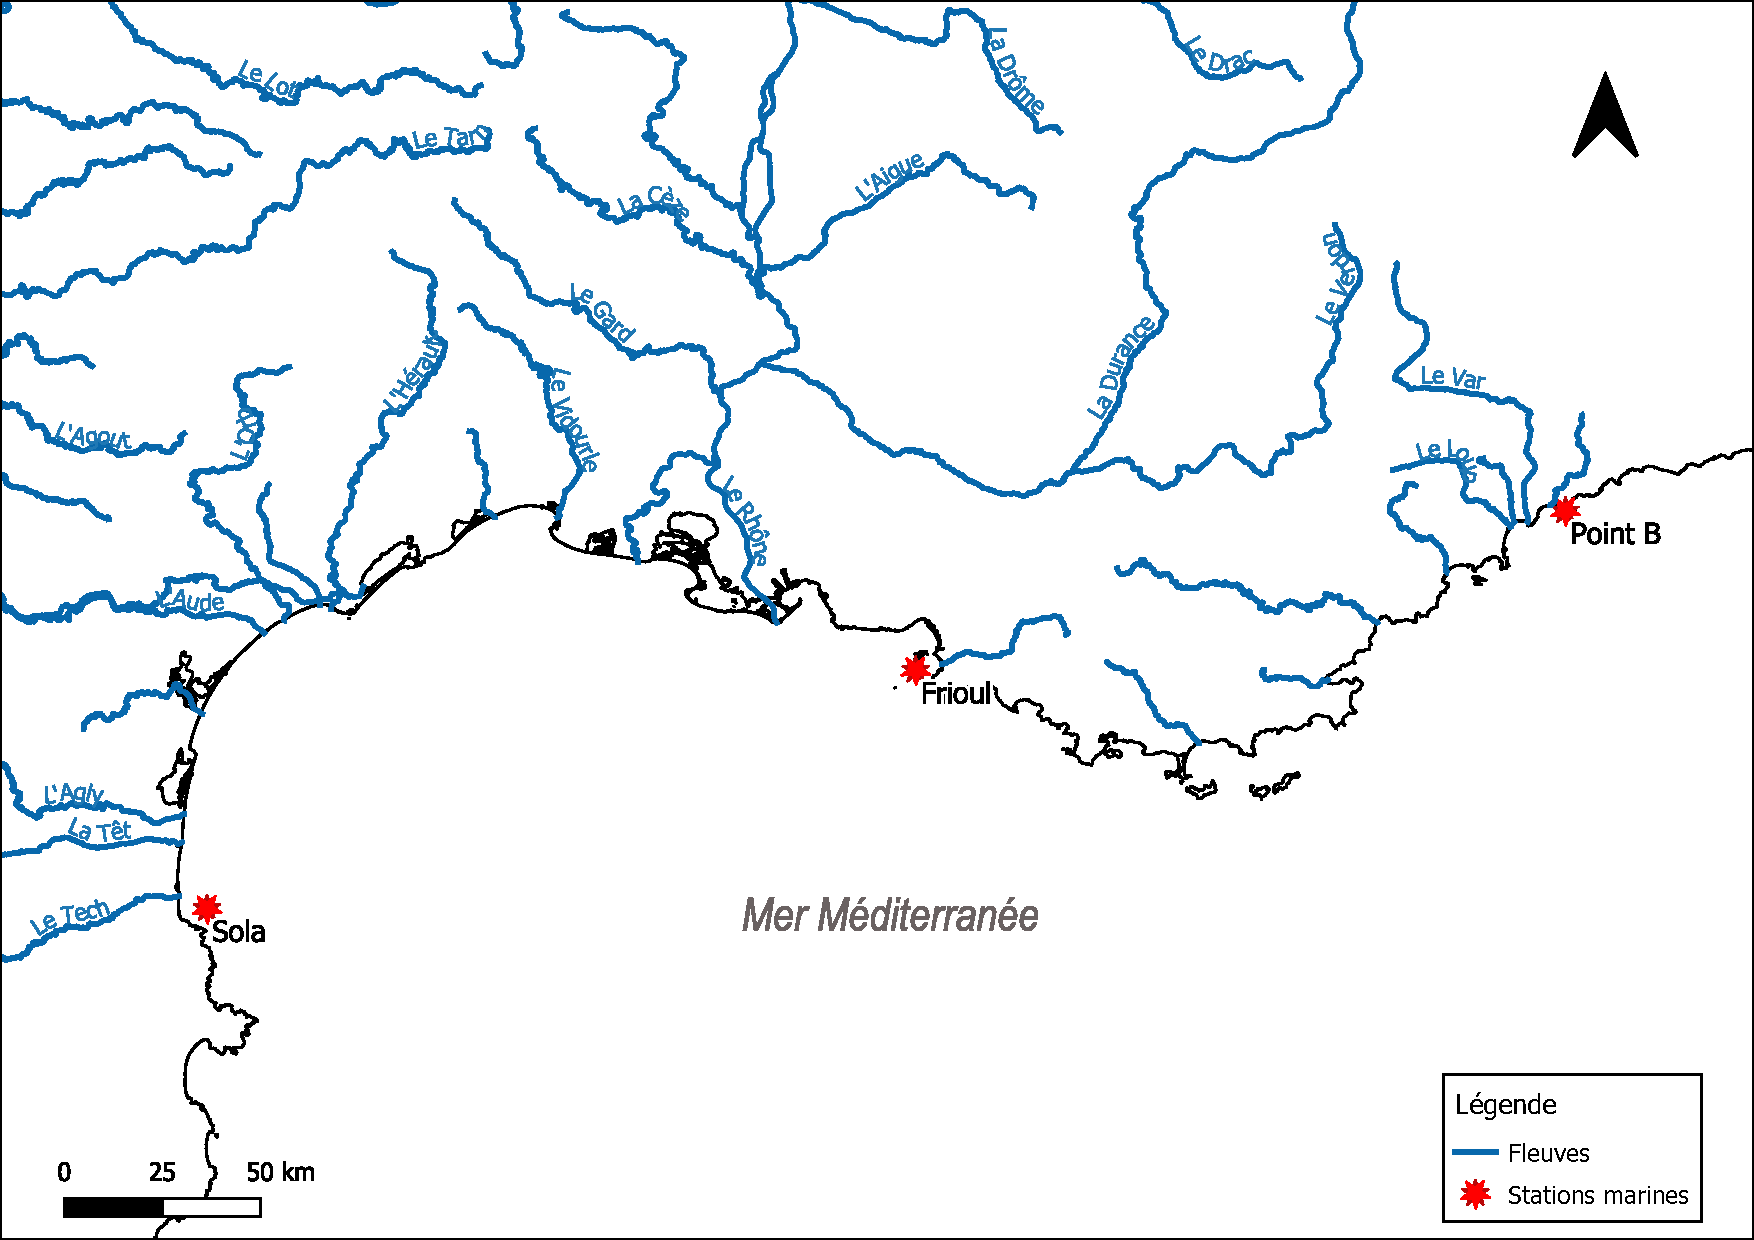
\includegraphics[width=.7\textwidth]{fig/MM_map.pdf}
\caption{Carte des stations SOMLIT méditerranéennes : Sola à Banyuls, Frioul à Marseille et Point B à Villefranche.}
\label{map}
\end{figure}

La station de Marseille, Frioul, se situe sur un fond sableux, sur 60m de profondeur à 5km de la côte. Cette station localisée dans le golfe de Marseille est considérée comme strictement marine. Cependant, la proximité du Rhône, l’un des fleuves les plus importants de la Méditerranée, fait que cette station subit une influence continentale marquée. 

La station de Villefranche, Point B, est située dans la Baie du Villefranche sur 80m de fond. Elle est abritée des vents d’est et d’ouest dominants dans la région. Les masses d’eau du large pénètrent dans la rade grâce au Courant Nord et à l’absence de plateau continental. Les apports d’eau douce les plus proches sont les fleuves Roya, Paillon et Var, avec de fortes variations saisonnières. Se site est également soumis à des influences anthropiques d’amplitude saisonnière. Il subit notamment un trafic maritime intense. 

% GG : [JE DEPLACERAIS CE PRARAGRAPHE DANS L'INTRO] De manière générale en Méditerranée, on observe la mise en place d’une thermocline saisonnière du printemps à l’automne. Ce phénomène est amplifié dans le Golfe du Lion où sont situées les stations Sola et Frioul \citep{Millot1990}. La circulation de surface dans le Golfe du Lion est dominée par le Courant Nord qui suit le talus continental le long de la côte de Provence et dans le Golfe du Lion jusque la Mer Catalane \citep{Millot1990}. Les vents dominants, le Mistral dans la région de Marseille et la Tramontane dans la région de Banyuls, sont des vents de nord-ouest.  Ils ont des conséquences sur le transport des sédiments ainsi que sur le déclenchement d’\textit{upwelling} à proximité de la côte. Ces vents peuvent également avoir un impact sur l’étendue du panache du Rhône qui est une source importante d’eau douce en Méditerranée. Cet apport continental peut conduire à la formation d’une couche d’eau douce de surface allant de quelques mètres à une dizaine de mètres de profondeur dans la région sous influence du Rhône \citep{Pairaud2011}. La Méditerranée étant de nature oligotrophe, les apports du Rhône ne sont pas négligeables et peuvent modifier de manière importante la productivité des organismes marins \citep{Pairaud2011}. %


\subsubsection{Prélèvements et protocoles}

L’acquisition des données est réalisée par des membres du SOMLIT lors de sorties en mer tous les 15 jours à Marseille et de manière hebdomadaire à Villefranche et à Banyuls. Depuis la création du SNO, des protocoles nationaux ont été établis progressivement. Aujourd’hui, les protocoles de prélèvements et d’analyses sont standardisés pour toutes les stations du SOMLIT. Cela permet une comparaison des observations entre les stations facilité et plus robuste. 

À chaque sortie en mer, l’eau est prélevée dans des bouteilles Niskin en surface (1m) et au fond à des profondeurs définies pour chaque station. Elles sont de 3m en surface et 24m de profondeur à Sola, 1m et 55m au Frioul, 1m et 50m au Point B. La température et la salinité sont alors mesurées. L’oxygène dissous est déterminé par la méthode de Winkler. De l’eau est échantillonnée des bouteilles Niskin pour réaliser une mesure en laboratoire du pH par spectrophotométrie. Un échantillonnage est également réalisé pour l’analyse de l’amonium (NH$_4$) par fluorimétrie. D’autre échantillonnages des bouteilles Niskin sont destinés à l’analyse des nutriments, nitrites (NO$_3$), nitrates (NO$_2$), phosphates (PO$_4$) et silicates (Si(OH)$_4$) par la méthode de Aminot et Kerouel (2004). La concentration de la matière en suspension (MES) est déterminée après filtration d’un échantillon dans des filtres de 0,7$\mu$m. Les concentrations en carbone organique particulaire (COP) et en azote organique particulaire (NOP) sont déterminées par combustion du matériel particulaire après filtration d’un échantillon. La chlorophylle \textit{a} est elle, déterminée par fluorimétrie d’un échantillon. Les protocoles détaillés sont disponibles sur le site du SOMLIT (https://www.somlit.fr/). 


Les profils verticaux sont réalisés avec une sonde \textit{conductivity-temperature-depth} (CTD SBE19plusV2, Seabird).  Elle permet de mesurer la température et la salinité dérivée de la conductivité. Couplée à un capteur de lumière biosphérique PAR, la radiation lumineuse est également mesurée par la CTD. Associée à un fluorimètre, elle permet aussi d’obtenir le profil de fluorescence en relation avec la concentration en chlorophylle-a. La sonde CTD est déployée entre la surface et le fond, en station, à chaque sortie en mer. Dans le cas de Villefranche, la sonde est déployée au Point B+ sur 150m de profondeur. 


L’eau prélevée à la surface dans une bouteille Niskin est également échantillonnée pour les analyses du pico et nano-plancton \citep{Marie2014} . L’échantillon est fixé avec un mélange de Glutaraldéhyde et Polaxamer, et est conservé jusqu’à son envoi à la plate-forme de Banyuls où tous les échantillons sont analysés par cytométrie en flux \citep{Marie2014}.

Lors de l’analyse par cytométrie, les cellules en suspension dans l’eau de mer filtrée passent une à une au travers d'un ou de plusieurs faisceaux laser. Les signaux de diffusion et de fluorescence émis par chaque cellule sont collectés par des détecteurs. La fluorescence émise par les cellules photosynthétiques provient principalement de leurs pigments photosynthétiques. Les longueurs d’ondes émises dépendent du type et de la concentration des pigments. La présence de chlorophylle induit une émission de fluorescence dans le rouge et la présence de phycoérythrine induit une émission dans l’orange. Dans le cas de cellules hétérotrophes, la seule fluorescence émise est la fluorescence verte induite par le marquage spécifique de l’ADN des cellules par le colorant SYBR Green I (Molecular probes). La diffusion lumineuse à 90 degrés est indicatrice de la structure (granularité) de la cellule \citep{Trask1982} et la diffusion de la lumière aux petits angles est en relation avec la taille de la particule \citep{Dubelaar2007}.

Les propriétés optiques des cellules mesurées par cytométrie en flux permettent de distinguer des groupes, formés par des cellules aux propriétés homogènes, dans la communauté pico et nano-planctonique. Néanmoins, ces groupes ne contiennent pas nécessairement chacun une unité taxonomique définie. Il est donc possible de distinguer les bactéries hétérotrophes, et parmi elles, celles à haut contenu en acide nucléique (bactéries HNA) et celles à faible contenu en acide nucléique (bactéries LNA). Parmi les organismes autotrophes il est possible de distinguer les \textit{Prochlorococcus}, les \textit{Synechococcus}, les Cryptophytes, les pico-eucaryotes et les nano-eucaryotes \citep{Marie1999}.

Les \textit{Prochlorococcus} et les \textit{Synechococcus} sont des procaryotes autotrophes. Ce sont des producteurs primaires particulièrement importants dans des conditions oligotrophes. Ils constituent des proies pour les Ciliés, les Dinoflagellés et le nano-plancton hétérotrophe \citep{Romagnan2015}. Les pico-eucaryotes autotrophes, d’une taille inférieur à 2$\mu$m, présentent une forte affinité pour les nutriments et la lumière, qui grâce à un ratio surface/volume élevé leur confère un avantage en condition oligotrophe \citep{LeQuere2005}. Les Cryptophytes sont des eucaryotes de taille hétérogène. Les nano-eucaryotes englobent tous les autres organismes autotrophes avec une taille comprise entre 2 et 20$\mu$m (Figure \ref{groupes}). 


\begin{figure}
\centering
\includegraphics[width=.7\textwidth]{fig/MM_res_troph.png}
\caption{Réseau trophique planctonique pélagique. Les groupes distingués par cytométrie en flux sont représentés par des cases qui englobent les organismes qu'ils peuvent contenir, en bleu foncé les bactéries hétérotrophes (BAC), en vert les \textit{Prochlorococcus} (PRO), en jaune les \textit{Synechococcus} (SYN) en bleu clair les pico-eucaryotes (PICOE), en gris les Cryptophytes (CRY) et en orange les nano-eucaryotes (NANOE). Modifié depuis \citet{Vage2015}.}
\label{groupes}
\end{figure}

\subsubsection{Jeux de données}

Les données collectées lors des campagnes du SOMLIT sont hébergées dans la base de données SOMLIT (https://www.somlit.fr/).  Les données hydrologiques, biologiques (cytométrie) et CTD pour les trois sites d’intérêt, Banyuls, Marseille et Villefranche, ont été téléchargées depuis le site internet.  Le Tableau \ref{data_table} résume les données récupérées pour les trois stations. Le jeu de données hydrologiques (HYDRO) contient les données de température, salinité, oxygène, pH, NH$_4$, NO$_3$, NO$_2$, PO$_4$, Si(OH)$_4$ , carbone (COP) et azote (NOP) organiques particulaires, , matière en suspension (MES) et  chlorophylle \textit{a}. Le jeu de données biologiques (PICONANO) contient les données de cytométrie des groupes de plancton présentés précédemment. Pour tous les groupes, les données d’abondance et de diffusion lumineuse moyenne des cellules sont disponibles. Pour le phytoplancton, sont de même disponibles les intensités moyennes d’auto-fluorescence rouge, et pour les bactéries hétérotrophes les intensités de fluorescence verte moyenne. Les valeurs d’auto-fluorescence orange de \textit{Synechococcus} et des Cryptophytes sont également renseignées. Le jeu de données CTD contient les profils verticaux de la surface au fond pour les variables température, salinité, chlorophylle \textit{a} et éclairement. 

\begingroup
\renewcommand*{\arraystretch}{1.5}
\begin{table}
\caption{Données téléchargées à partir du site internet du SOMLIT pour les trois stations méditerranéennes. Résume le nombre d'observations disponibles (N) pour chaque site en fonction de la profondeur de l'échantillonnage (Prof).}
\label{data_table}
\begin{tabularx}{\textwidth}{X l l X l l X l l l}
\hline
Station & \multicolumn{3}{c}{Données HYDRO} & \multicolumn{3}{c}{Données PICONANO} & \multicolumn{3}{c}{Données CTD} \\
\hline
 & Début & N & Prof (m) & Début & N & Prof (m) & Début & N & Prof (m)\\
\hline
Banyuls &1997 & 1183 & 3  & 2012 & 215 & 3 & 2019 & 93 & 3-24\\
& 1997 & 1184 & 24 & & & & \\
Marseille &1997 & 583 & 1 & 2012 & 213 & 1 & 1994 & 627 & 0-55\\
& 2004 & 407 & 55 & & & & \\
Villefranche  & 1995 & 1320 & 1 & 2012 & 192 & 1 & 2007 & 634 & 1-150\\
& 1995 & 1321 & 50 & & & & \\
\hline
\end{tabularx}
\end{table}
\endgroup

Une première visualisation des données permet d’identifier % les séries temporelles exploitables et les éventuelles%
les données aberrantes. La Figure \ref{vis_hydro} présente les données de surface des variables hydrologiques au cours du temps toutes stations confondues. Les éventuelles valeurs aberrantes sont identifiées en rouge. La ligne pointillée orange correspond au début du jeu de données cytométriques PICONANO et la lignée pointillée bleue correspond à la mise en place du protocole national pour la variable présentée. Étant donné la mise en place tardive d’un protocole standardisé pour le pH, cette variable n’est pas analysée. La mesure de l’oxygène étant sujette à de nombreux biais liés à la précision de l’échantillonnage, celle-ci est également ignorée. La Figure \ref{vis_T} présente les données de température de surface et au fond pour les trois stations. Les graphiques nous permettent d’identifier une potentielle inversion des données de fond et de surface à Villefranche entre le début de la série temporelle et 2002. Comme il est impossible de savoir avec certitude quelles observations ont été interverties, les données HYDRO de Villefranche datant d’avant  2002 ne sont pas exploitées. 

\begin{figure}
\centering
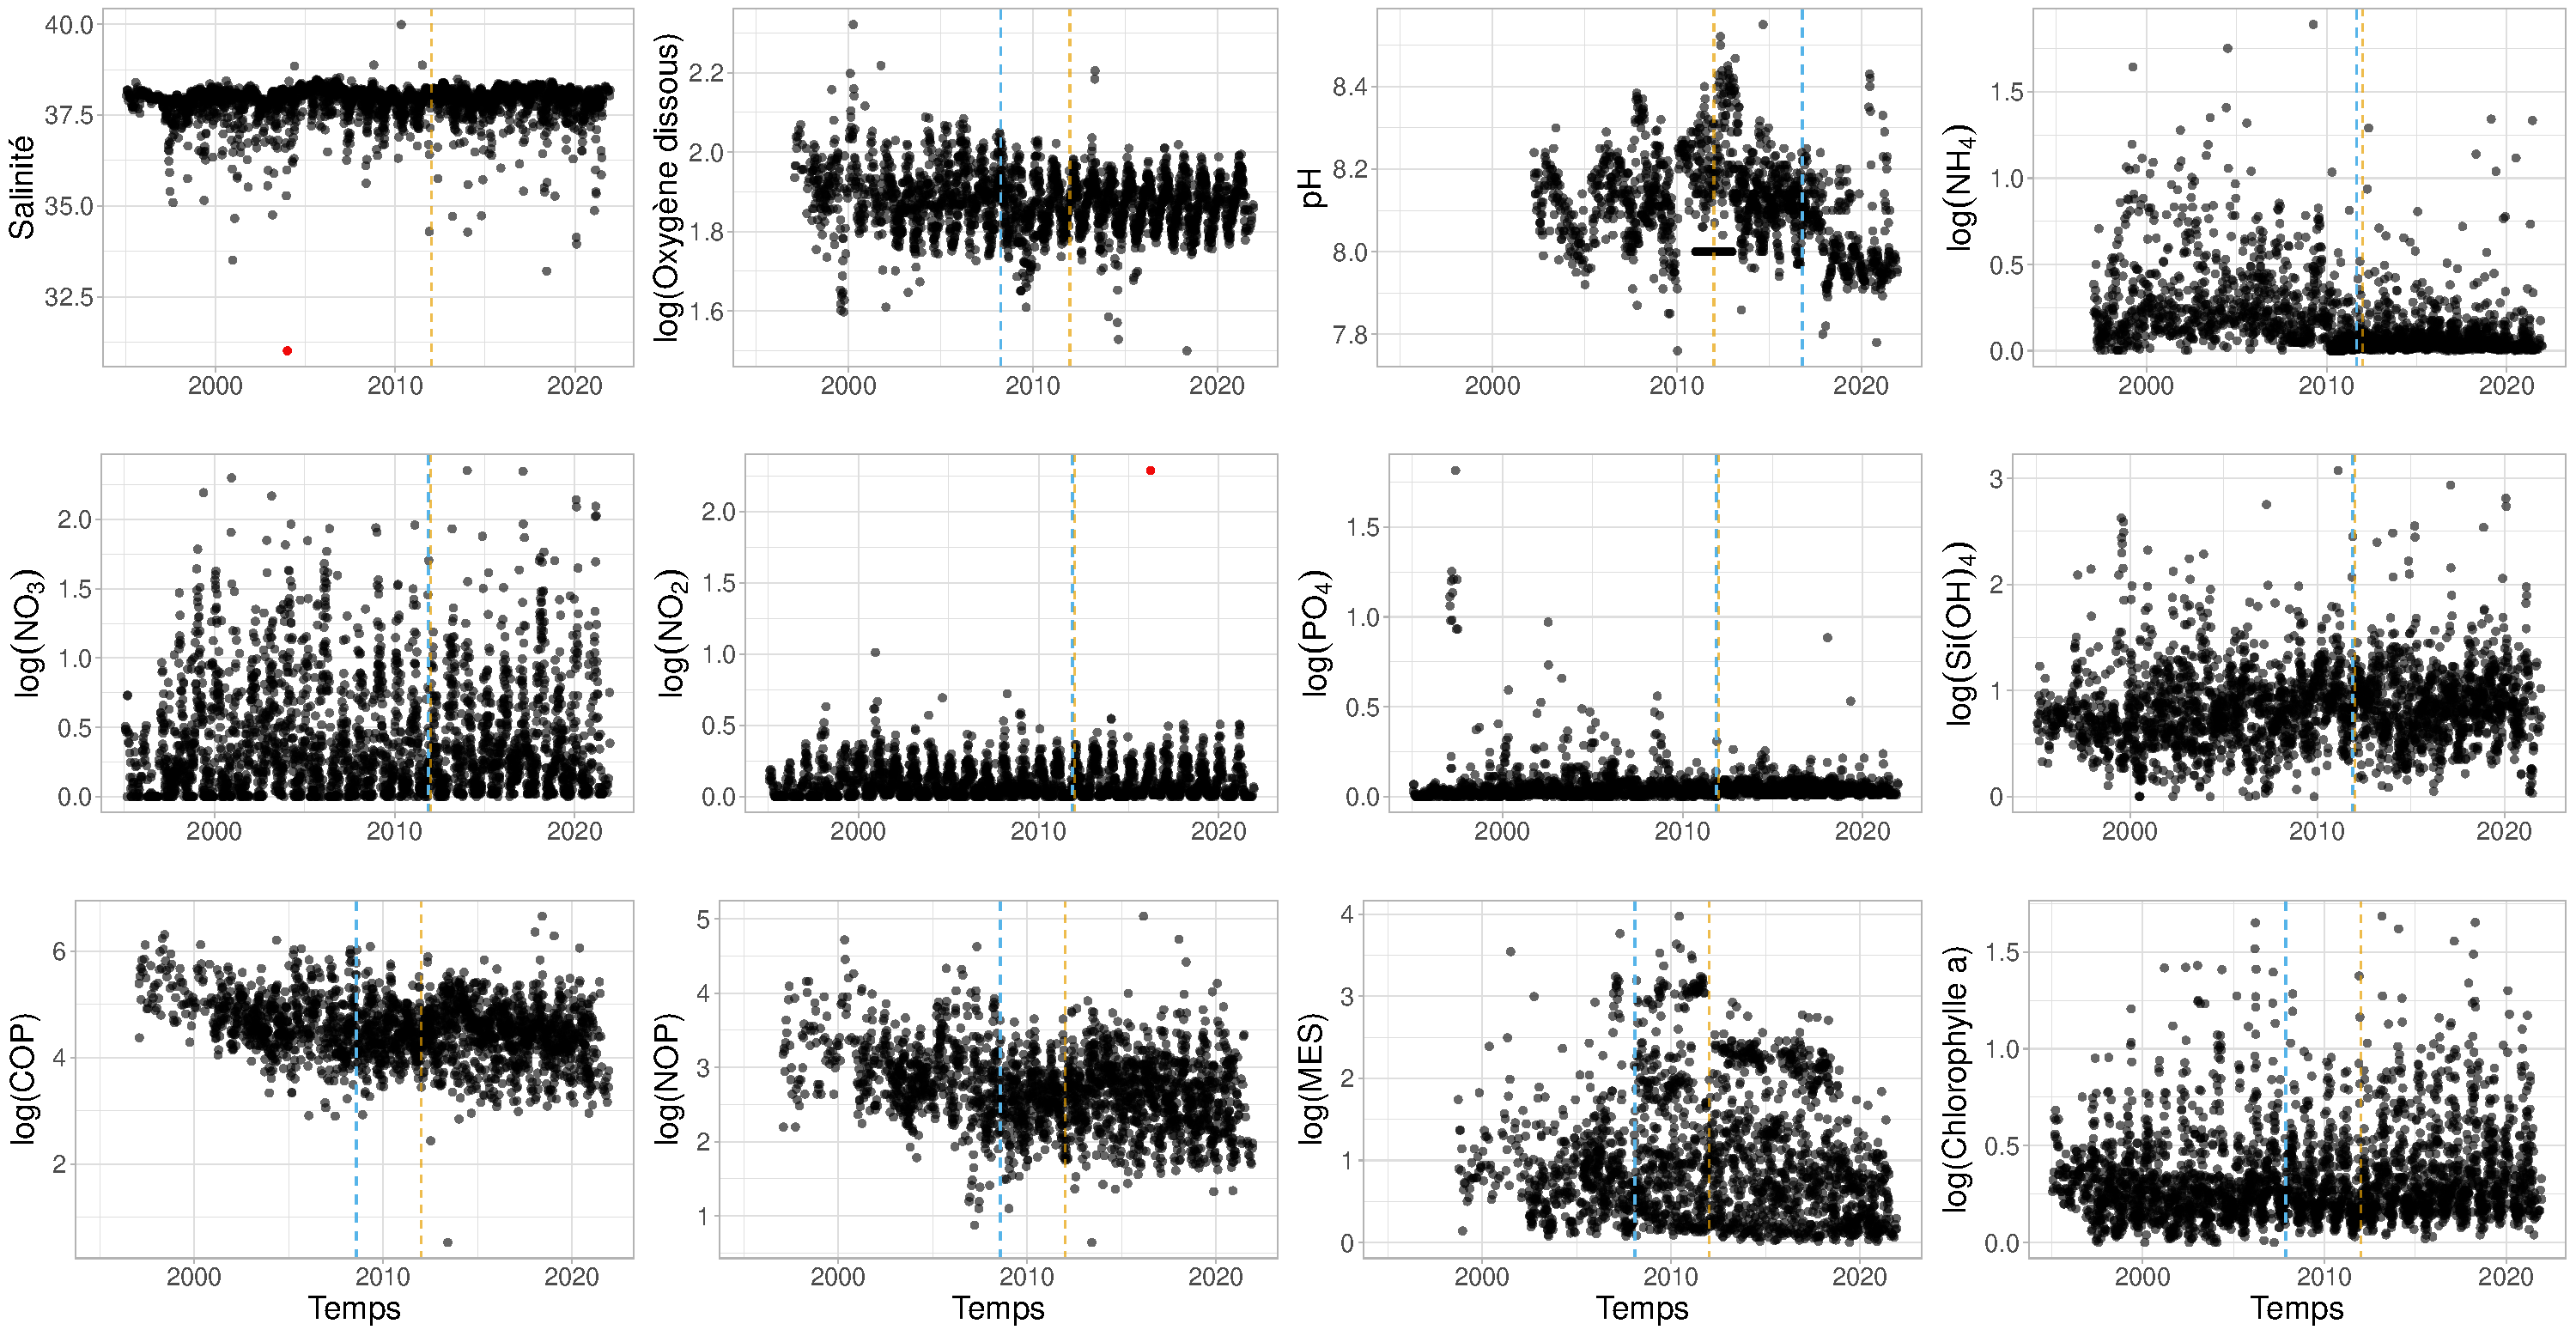
\includegraphics[width=\textwidth]{fig/MM_visualisation_hydro.pdf}
\caption{Séries temporelles des données hydrologiques de surface pour les trois stations SOMLIT méditerranéennes confondues. La ligne pointillé bleue correspond à la mise en place du protocole national pour la variable présentée. La ligne pointillée orange correspond au début du jeu de données PICONANO. Les éventuelles données aberrantes sont représentées en rouge.}
\label{vis_hydro}
\end{figure}

\begin{figure}
\centering
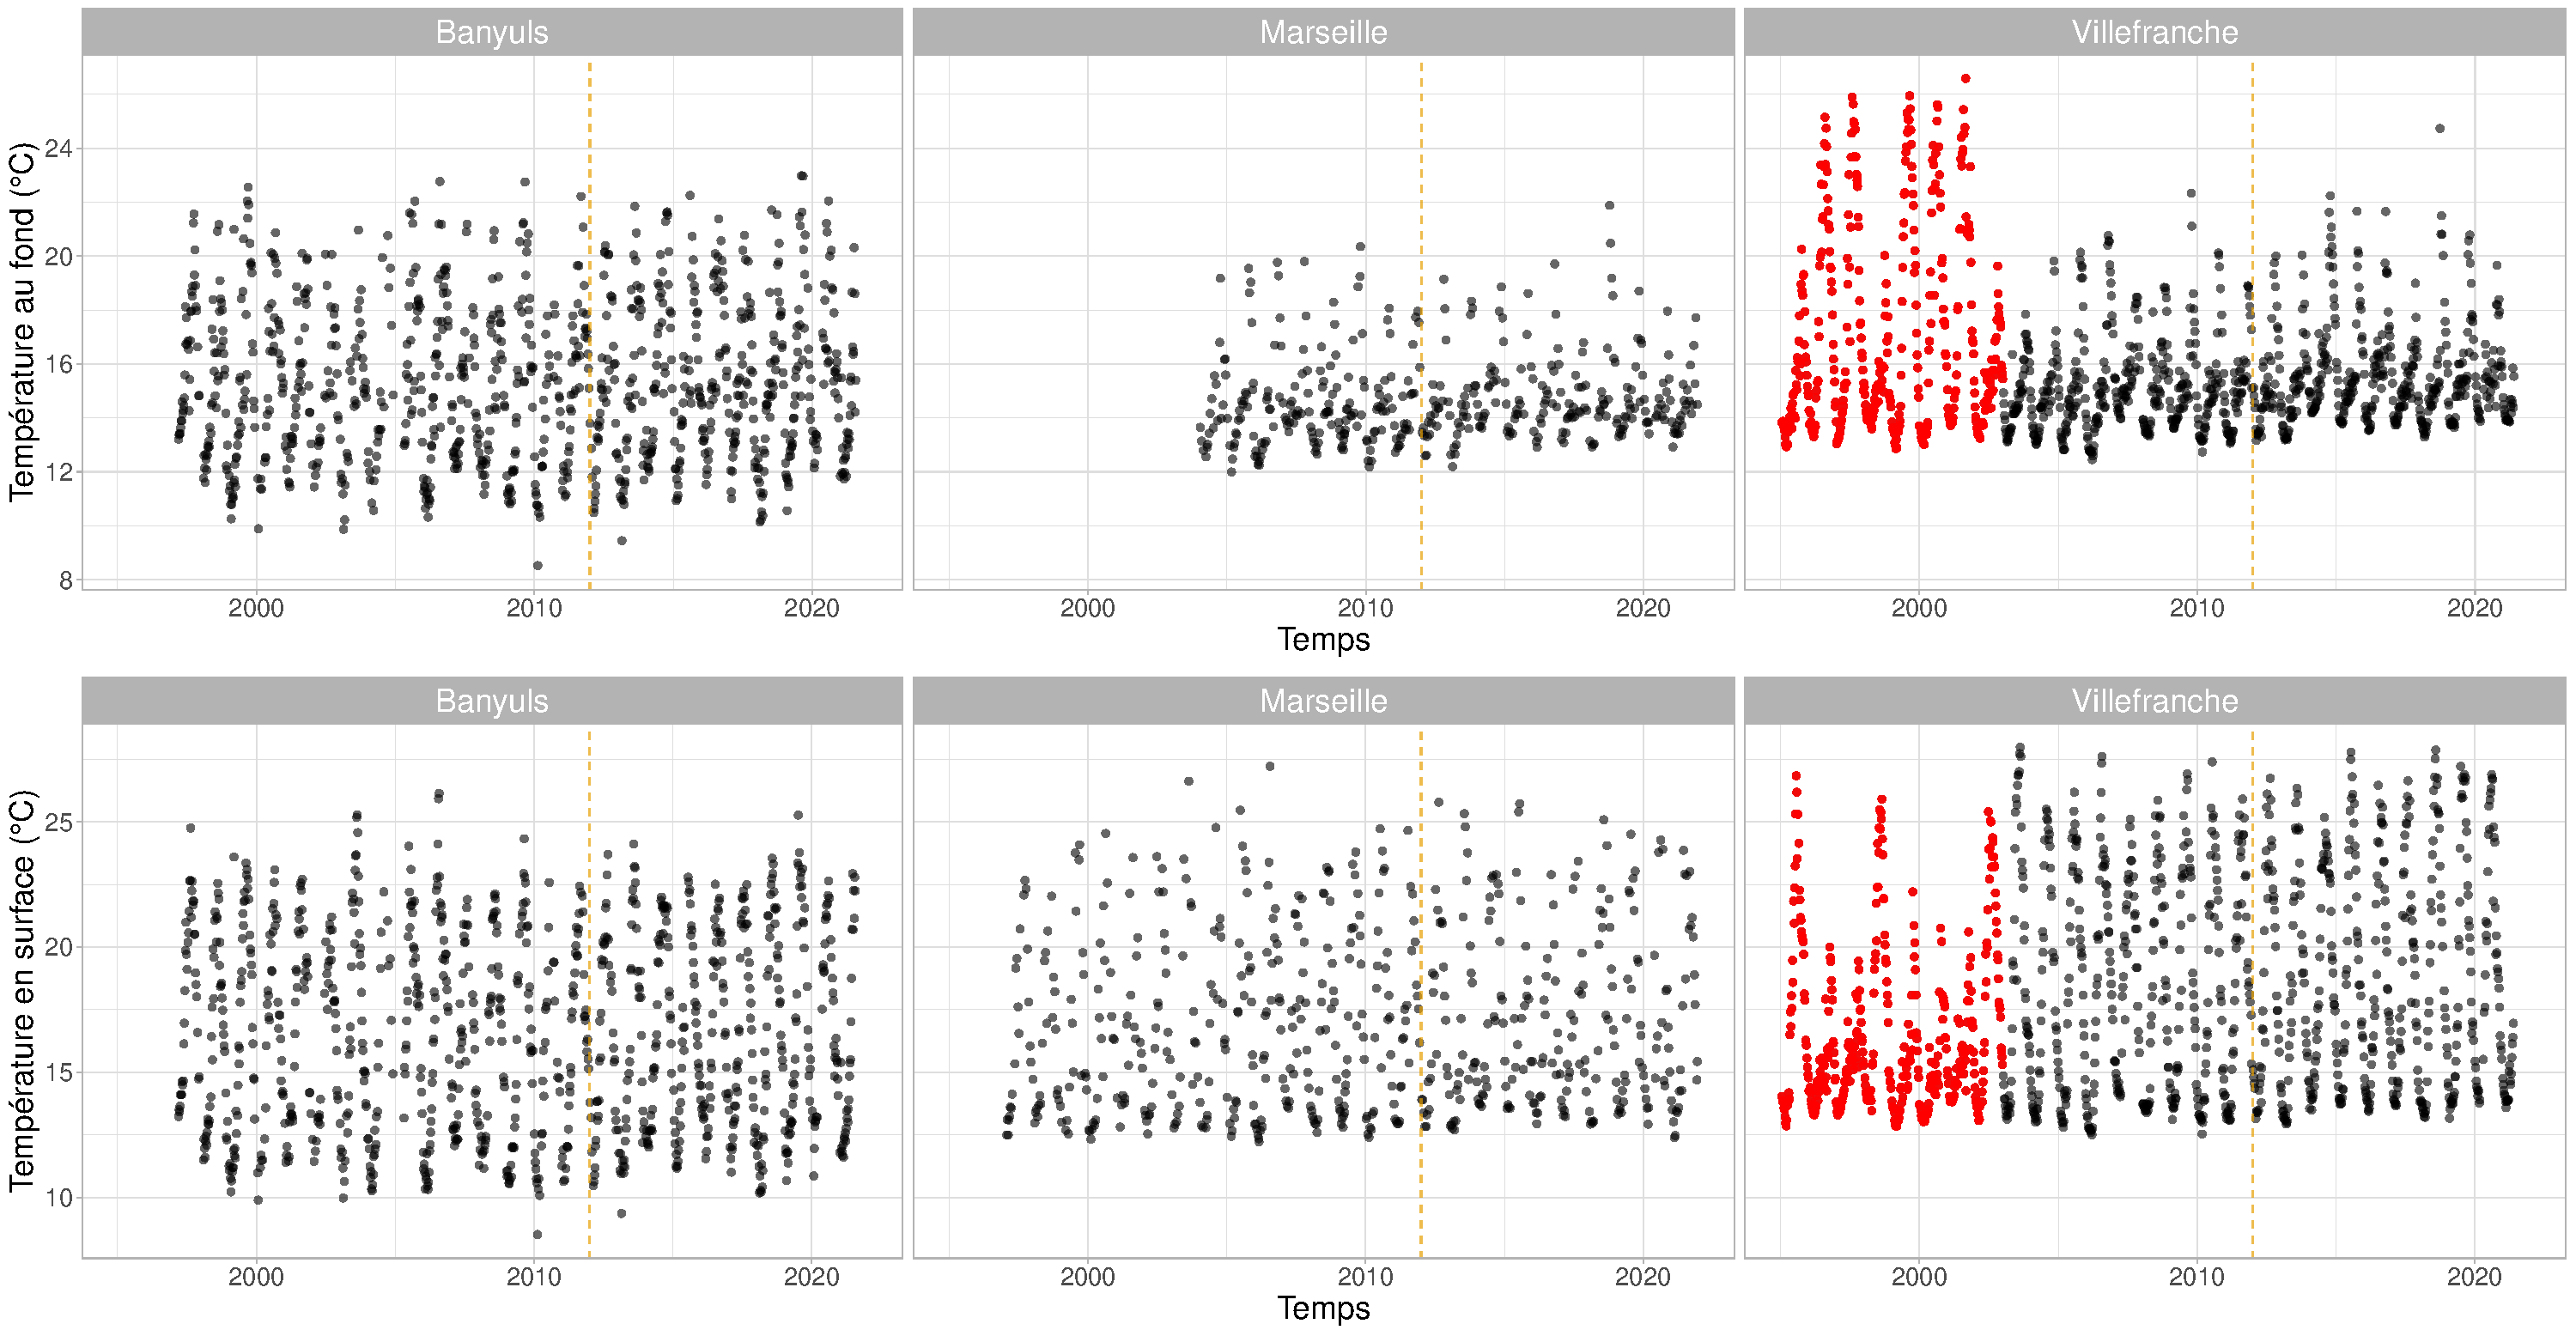
\includegraphics[width=.9\textwidth]{fig/MM_visualisation_T.pdf}
\caption{Séries temporelles des données de température en surface et au fond pour les trois stations méditerranéennes. La ligne pointillée orange correspond au début du jeu de données PICONANO. Les éventuelles données aberrantes sont représentées en rouge.}
\label{vis_T}
\end{figure}

Dans le cadre de ce stage, nous nous sommes focalisés sur le phytoplancton. Par soucis de temps, les bactéries hétérotrophes ne sont pas prises en compte. 
La combinaison des propriétés optiques des cellules mises en évidence par la cytométrie en flux, permet de distinguer des groupes dans la communauté phytoplanctonique. % Si la fluorescence rouge à la chlorophylle présente une gamme étendue de valeurs au sein d’une communauté, sa variabilité reste faible au sein d’une même espèce \citep{Trask1982}. Ainsi, la fluorescence à la chlorophylle peut être utilisée pour distinguer des espèces. L’association de la fluorescence rouge à la diffusion lumineuse, indicatrice de la taille et de la structure des cellules, devrait donc permet\-tre d’identifier les groupes décrits précédemment.
La Figure \ref{vis_cyto} représente avec une échelle logarithmique, la valeur moyenne d’auto-fluorescence rouge d’un groupe lors d’un prélèvement, en fonction de la valeur moyenne de diffusion lumineuse. À l’exception d’une observation pour le groupe de \textit{Synechococcus} isolée de toutes les autres, les données paraissent fiables puisque l'on identifie facilement les différents groupes. 

\begin{figure}
\centering
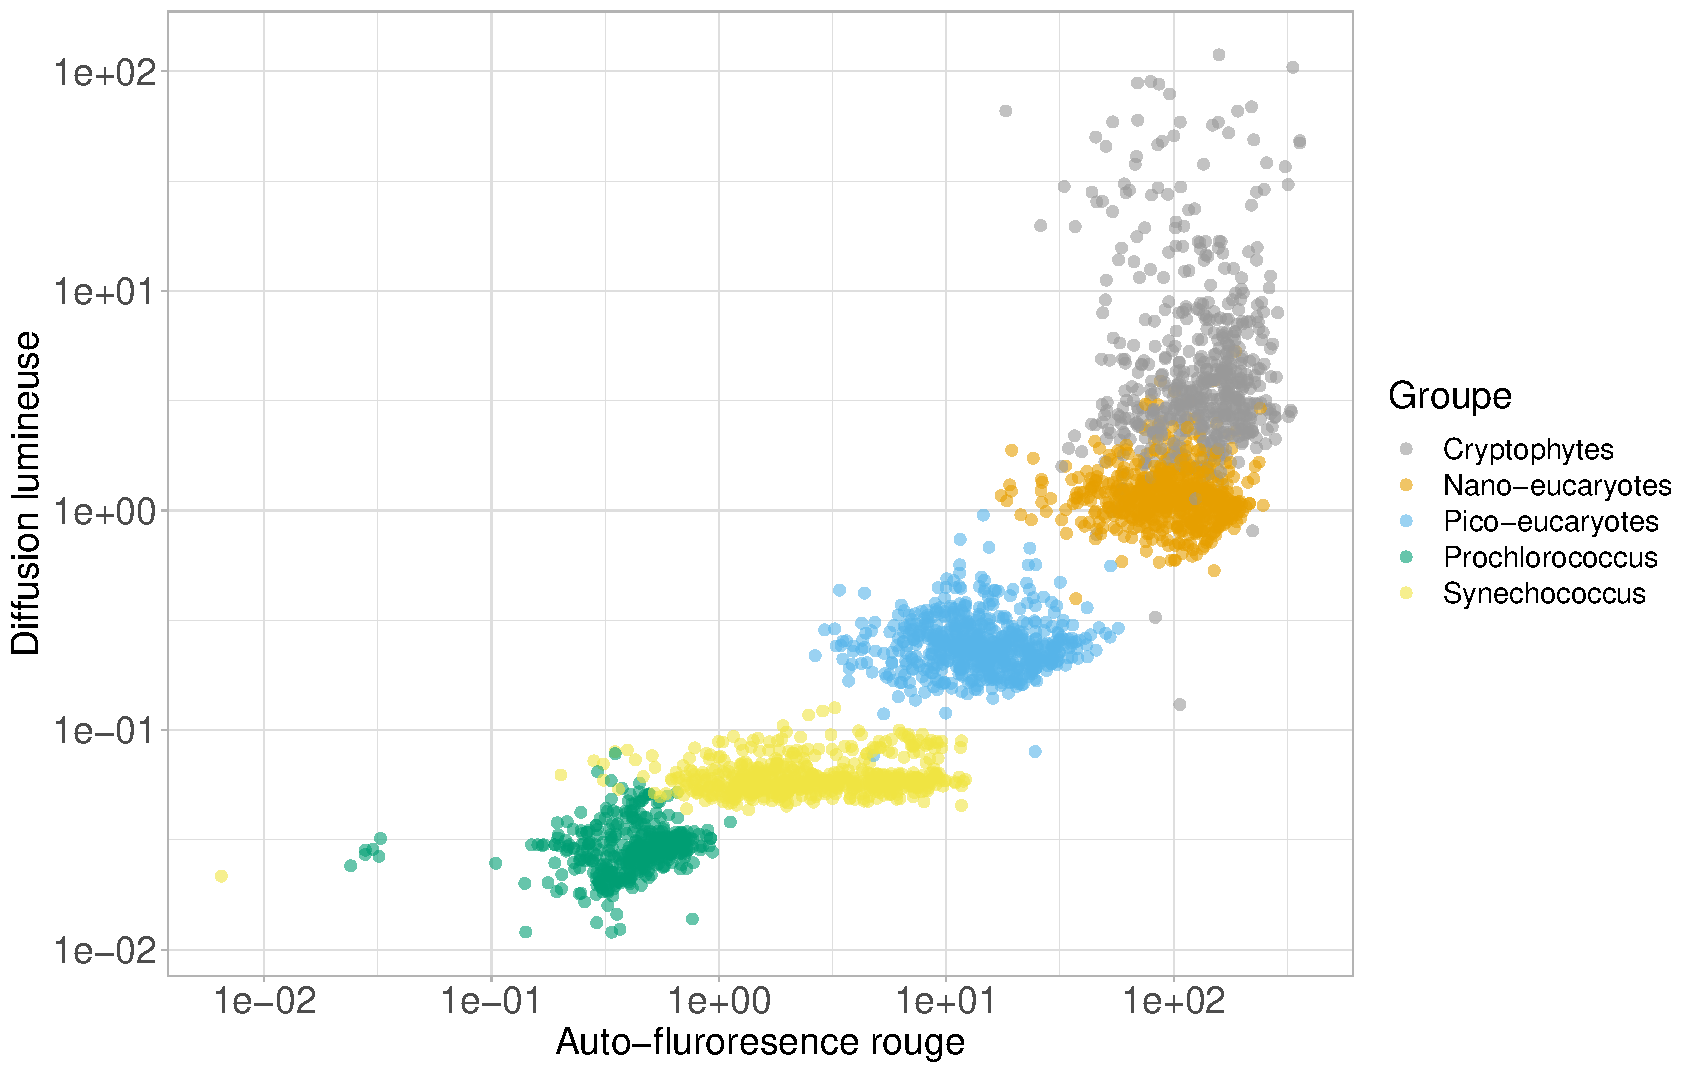
\includegraphics[width=.75\textwidth]{fig/MM_visualisation_phyto.pdf}
\caption{Auto-fluorescence rouge moyenne \textit{versus} diffusion lumineuse à 90° moyenne de chaque groupe de phytoplancton pour chaque prélèvement pour les trois stations SOMLIT méditerranéennes. }
\label{vis_cyto}
\end{figure}

En ce qui concerne les données PICONANO, % toutes les variables semblent exploitables et pourraient potentiellement apporter des informations pertinentes. Néanmoins, 
durant ce stage l’étude s'est focalisée sur les variables d’abondance et de diffusion lumineuse (SSC), cette dernière étant indicatrice de la structure des organismes. 

\subsection{Analyse de séries temporelles}

La visualisation et l’étude de l’évolution des populations au cours du temps sur toute la durée de la période d’étude peut constituer une première étape pour déceler les  tendances et comprendre la dynamique temporelle que suit chaque population. De plus, dans le contexte du réchauffement, il convient d’étudier la tendance que suit la température au cours du temps au sein des stations. La durée d’observations des données de 10 ans pour les données biologiques et plus pour les données hydrologique, rend possible l’étude de l’évolution des variables au cours du temps. Ces variables peuvent donc être étudiées avec des méthodes d’analyse de séries temporelles. 

\subsubsection{Lissage non-paramétrique}

Afin d'explorer les séries temporelles pour identifier une structure et déceler une éventuelle tendance, dans un premier temps, un lissage a été réalisé sur chaque variable d’intérêt et pour chaque station. Le choix du lissage non paramétrique est fait car nous ne connaissons pas la structure des séries et que c’est justement ce que nous cherchons à identifier.

Un modèle de régression non-paramétrique peut s'écrire de la manière suivante : 
\[y_i=m(x_i) + \epsilon_i\]

Avec $m(x)$ la courbe de régression qui correspond à l'espérance conditionnelle $E(Y|X=x)$. Il est possible de définir un estimateur à noyau de cette courbe. De telle manière qu’aux valeurs de $y$ correspondant aux points $x_i$ les plus proches de $x$ est accordé un poids plus important. Dans le cas où le voisinage est large, il convient d'utiliser des polynômes d’ordre $p$. Dans ce cas, un estimateur par régression polynomiale locale $\hat{m}_p(x)$ correspond à  $\hat{\beta}_0$ qui minimise l’équation suivante \citep{Simonoff1996}.

\[\sum_{i=1}^n\big(y_i-\beta_0-...-\beta_p(x-x_i)^p\big)^2K\Big(\frac{x-x_i}{h}\Big)\]

On fait le choix d'utiliser un noyau $K()$ gaussien, non-borné qui permet d'avoir une variance conditionnelle finie \citep{Simonoff1996}. L'ordre des polynômes est fixé à 2 car un degré supérieur n'apporte pas une précision significativement meilleure. Le choix de la fenêtre de lissage $h$ est fait en testant plusieurs valeurs. Nous conservons celle qui permet une bonne estimation des observations réelles tout en produisant une régression suffisamment lisse. 

L'intervalle de confiance à 95\% de la régression est calculé à partir de la méthode décrite par \citet{Fan1996}. Cette méthode se base sur l’expression asymptotique du biais et de la variance conditionnels. Dans cette étude, ils sont approximés par un développement de Taylor d’ordre 1. 

\subsubsection{Saisonnalité}

Pour déterminer %une éventuelle
la saisonnalité dans les séries temporelles, nous nous sommes intéressés à la densité spectrale. La densité spectrale est analogue à une densité de probabilité. Elle donne la même information que la fonction d’auto-covariance. Cependant, au lieu d’exprimer la covariance en terme de \textit{lag}, elle l’exprime en terme de cycle. La densité spectrale peut être estimée par un périodogramme. 

Le périodogramme $P(\omega)$ indique quelles composantes de fréquences ont une grande magnitude et lesquelles ont une faible magnitude. De grandes valeurs de $P(\omega)$ indiquent donc quelles fréquences $\omega$ sont prédominantes dans la série. Les petites valeurs de $P(\omega)$ sont plus susceptibles d'être associées au bruit. 

La première étape consiste à s'affranchir de la tendance présente dans la série. En effet, les tendances vont donner de l'importance à des composantes de basses fréquences qui vont obscurcir les plus hautes fréquences. Nous réalisons donc un centrage des données de la forme $x_t-\bar{x}$ en amont de l’analyse. Le périodogramme peut ensuite être obtenu avec la transformation de Fourier rapide (FFT) \citep{Shumway2016}. 

Cependant, le périodogramme est sujet à de nombreuses incertitudes. Pour que le périodogramme soit un estimateur fiable de la densité spectrale, il convient de lisser le périodogramme \citep{Shumway2016}. 


Le périodogramme lissé, ou périodogramme moyen $\bar{f}(\omega)$, est défini comme la moyenne des valeurs du périodogramme sur la bande de fréquence $\mathcal B$. Les valeurs du spectre à l'intérieur de cette bande doivent être relativement constantes pour que le spectre lissé soit un bon estimateur. La largeur de cette bande est ajustée par le choix de la fenêtre. Nous pouvons obtenir une approximation d'un intervalle de confiance à $100(1-\alpha)\%$ de la valeur du spectre $f(\omega)$ de la forme \citep{Shumway2016} :

\[\frac{df\bar{f}(\omega)}{\chi_{df}^2(1-\alpha/2)}\leq f(\omega) \leq \frac{df\bar{f}(\omega)}{\chi_{df}^2(\alpha/2)}\] 

Il est commun d'observer des pics mineurs au niveau des harmoniques car la plupart des signaux ne sont pas des sinusoïdes parfaits. Les harmoniques permettent alors de capturer le comportement non-sinusoïdal du signal. La question est de décider si un pic est significatif ou non. En général, un pic est considéré significatif si sa borne inférieure de l’intervalle de confiance est supérieure au bruit. 

Lors de la création de fenêtre, il est possible que certaines fréquences en dehors de l'intervalle voulu contaminent la bande. Pour supprimer cet effet de fuite, il est possible d'utiliser des \textit{taper}. Les \textit{taper} ont généralement une forme qui amplifie le centre des données par rapport aux extrémités, comme par exemple une cloche cosinus \citep{Shumway2016}.

Le périodogramme moyen est calculé à l’aide du paquet $astsa$. Il permet d’ajouter un taper de la forme d’une cloche cosinus et d’ajuster le noyau. Le noyau choisi est celui qui produit un périodogramme moyen le plus ressemblant au périodogramme échelonné. 


\subsection{Analyse en Composantes Principales Fonctionnelle}

Une Analyse en Composantes Principales (ACP) classique a pour objectif de trouver les combinaisons linéaires de variables quantitatives qui maximisent la variance au sein d’un jeu de données. Notre intérêt se porte, non pas sur des observations ponctuelles, mais sur l’évolution dans le temps ou dans l’espace de ces observations. Cette évolution peut être modéliser par des fonctions. Si une fonction peut être exprimée par des coefficients, il suffit de chercher alors les combinaisons linéaires de ces coefficients qui maximisent la variance entre ces fonctions. C’est le principe de l’ACP fonctionnelle. 

\subsubsection{Lissage paramétrique}

La première étape consiste à transformer des données d’échantillonnages discrètes en des fonctions continues sur l’intervalle que nous souhaitons comparer. Dans le cas des données HYDRO et PICAONANO nous nous intéressons à des unités annuelles, une fonction correspond donc à une année. Dans le cas des données CTD, une fonction correspond à un profil vertical de mesures à une date d’échantillonnage.   

Pour obtenir une fonction $x(t)$, un système de fonctions de bases est utilisé. C'est un ensemble de $K$ fonctions $\phi_k$ connues et indépendantes les unes des autres. Une association linéaire de ces $K$ fonctions permet d'approximer notre fonction. La fonction $x(t)$ s'exprime alors comme une expansion linéaire : 

\[x(t)=\sum_{k=1}^Kc_k\phi_k(t)\]

Les coefficients d'expansion sont notés $c_k$.

La méthode de lissage choisie est celle par pénalisation de la courbure ou régularisation. Cette méthode de lissage permet de choisir le paramètre de lissage. Le paramètre de lissage $\lambda$ nous permet de contrôler l'équilibre entre l'ajustement de la courbe lissée aux données initiales et la variabilité de cette courbe. Une méthode subjective est utilisée : elle consiste à tester plusieurs valeurs de $\lambda$ et à sélectionner celle pour laquelle le lissage est le plus adapté. Des splines cubiques ont été choisies comme fonctions de bases, comme suggéré par \citet{Ramsay1998}.

\subsubsection{ACP fonctionnelle}

L'ACP fonctionnelle est réalisée avec le paquet $fda$. À la différence d’une ACP classique, au lieu de disposer de réalisations de $J$ variables, pour $N$ échantillons, nous allons étudier $N$ fonctions $x_i(t)$. Ce sont les coefficients d’expansion des fonctions $x_i(t)$ qui font office de variables. Dans le cas où il manque une moyenne mensuelle pour plusieurs années, l’ACP est réalisée avec le paquet $fdapace$ qui supporte les valeurs non attribuées.

\subsubsection{Perturbation de la moyenne}

Pour interpréter visuellement les résultats de l’ACP fonctionnelle, une solution est d'exprimer ses composantes principales comme perturbation de la moyenne $\hat{\mu}(t)$. Soit $\lambda_l$ la valeur propre de la $l$-ième composantes principales et $\hat{\xi}_l(t)$ sa fonction propre associée, il est possible de les exprimer de la manière suivante \citep{Nerini2021} : 

\[\hat{\mu}(t) \pm \sqrt{\lambda_l}\times \hat{\xi}_l(t)\]


\subsection{Analyse Factorielle Discriminante}

L’Analyse Factorielle Discriminante (AFD) est une méthode de classification supervisée. C’est à dire qu’elle permet de classer des observations en $K$ classes connues. Elle peut être utilisée comme une méthode descriptive qui permet d’identifier les variables quantitatives qui discriminent au mieux les $K$ modalités d’une variable qualitative. Cette méthode est utilisée pour tenter de discerner les trois stations méditerranéennes ($K=3$) en fonction de l’abondance de chaque groupe de phytoplancton, de la taille des organismes de chaque groupe de phytoplancton ou de la concentration de chaque nutriment, au cours d’une année. Le nombre d’axes discriminants d’une AFD est inférieur ou égale à $K-1$. Il est alors possible de visualiser les résultats de l’AFD en deux dimensions, en ayant toutes les informations.  

Une étape préliminaire à l’AFD consiste à passer des observations ponctuelles au cours d’une année à une observation qui correspond à l’évolution d’une variable au cours d’une année. Cette transformation est réalisée à l’aide d’ACP fonctionnelles présentées précédemment. Une ACP est réalisée pour chaque variable d’intérêt. Les variables qualitatives utilisées pour l’AFD correspondent aux scores des composantes principales des ACP. Selon le pourcentage d’inertie des composantes principales, une ou deux composantes principales sont récupérées pour chaque ACP. Si deux composantes principales sont récupérées, la deuxième est pondérée en fonction de son pourcentage d’inertie. 

Nous obtenons ainsi de nouvelles observations correspondant chacune à une année pour un site. Pour chaque observation, il y a $p \times j$ variables quantitatives qui correspondent aux scores des $p$ composantes principales de $j$ ACP. 

Dans le cas où l’on a des variables non-attribuées, la fonction $inputePCA$ du paquet $missMDA$ est utilisée. Cette fonction permet de simuler les valeurs manquantes en ajustant une valeur initiale, qui correspond à la moyenne de la variable, à l’aide d’ACP successives. Cette méthode peut être utilisée comme méthode préliminaire à une ACP \citep{Josse2012}. Or, une AFD est assimilable à une ACP particulière, avec ici 2 axes discriminants ($K-1$). Le nombre de composantes principales utilisées pour prédire les valeurs manquantes est donc fixé à 2. 

Une fois le tableau d’observations centré et réduit, l’AFD est réalisée avec la fonction $lda$ du paquet $MASS$.

\subsection{Analyse Canonique des Corrélations}

L’Analyse Canonique des Corrélations (ACC) est une méthode pour explorer les corrélations entre deux jeux de données quantitatives issues du même échantillonnage \citep{Gonzalez2008}. Les variables canoniques sont des combinaisons linéaires de variables d’un jeu de données. Une paire de variables canoniques est constituée d’une variable canonique venant du premier jeu de données et d’une autre venant du second jeu de données. L'ACC fonctionne comme un algorithme itératif visant à trouver les combinaisons linéaires qui maximisent la corrélation entre ces variables canoniques (corrélation canonique) \citep{Gonzalez2008}. 

L'ACC est utilisée pour explorer les corrélations entre les données biologiques et les données hydrologiques. Dans un premier temps, nous nous intéressons aux relations entre les données d’abondance et les concentrations en nutriments, dans un second temps à un possible lien entre les valeurs de SSC et les concentrations en nutriments.  

Comme pour l’AFD, nous allons nous intéresser à l’évolution d’une variable au cours d’une année. Nous avons donc recours aux scores des ACP utilisés lors de l’AFD. Au cours des analyses, nous avons remarqué que, souvent, la première composante principale rend compte d’un effet moyen. Si c’est en effet le cas, nous récupérons uniquement le score de la première composante principale. Le premier jeu de données $n \times p$ contient $n$ observations correspondant à une année, à un site. Et $p$ variables quantitatives qui correspondent aux scores des premières composantes principales issues des ACP pour chaque groupe de phytoplancton. Dans le premier cas il s’agit des variables d’abondance et dans le second cas des variables de diffusion lumineuse.  Le deuxième jeu de données $n \times q$ contient $n$ observations correspondant aux mêmes années aux mêmes sites que le premier jeu de données. Les $q$ variables quantitatives correspondent cette fois aux scores des premières composantes principales issues des ACP pour chaque nutriment.

L'ACC est réalisée avec le paquet $CCA$ qui supporte les valeurs manquantes. 


\section{Résultats}

\subsection{Variations dans le temps}

\subsubsection{Abondance des groupes phytoplanctoniques}

Comme nous disposons de données échantillonnées plus ou moins régulièrement deux fois par mois, nous souhaitons lisser les données pour avoir une évolution continue de l'abondance des groupes de phytoplancton au cours du temps.  

Pour chaque groupe phytoplancton défini par cytométrie, et pour chaque station, une régression polynomiale locale sur les observations d’abondance est réalisée pour transformer les données discrètes en fonctions continues. Après avoir essayé plusieurs fenêtres de lissage, celle qui convient le mieux pour chacune des régressions est une fenêtre de 40 jours. Les lissages obtenus sont présentés en Figure \ref{ts_ab}. Toutes les séries présentent une saisonnalité annuelle plus ou moins marquée. 

\begin{sidewaysfigure}[p]
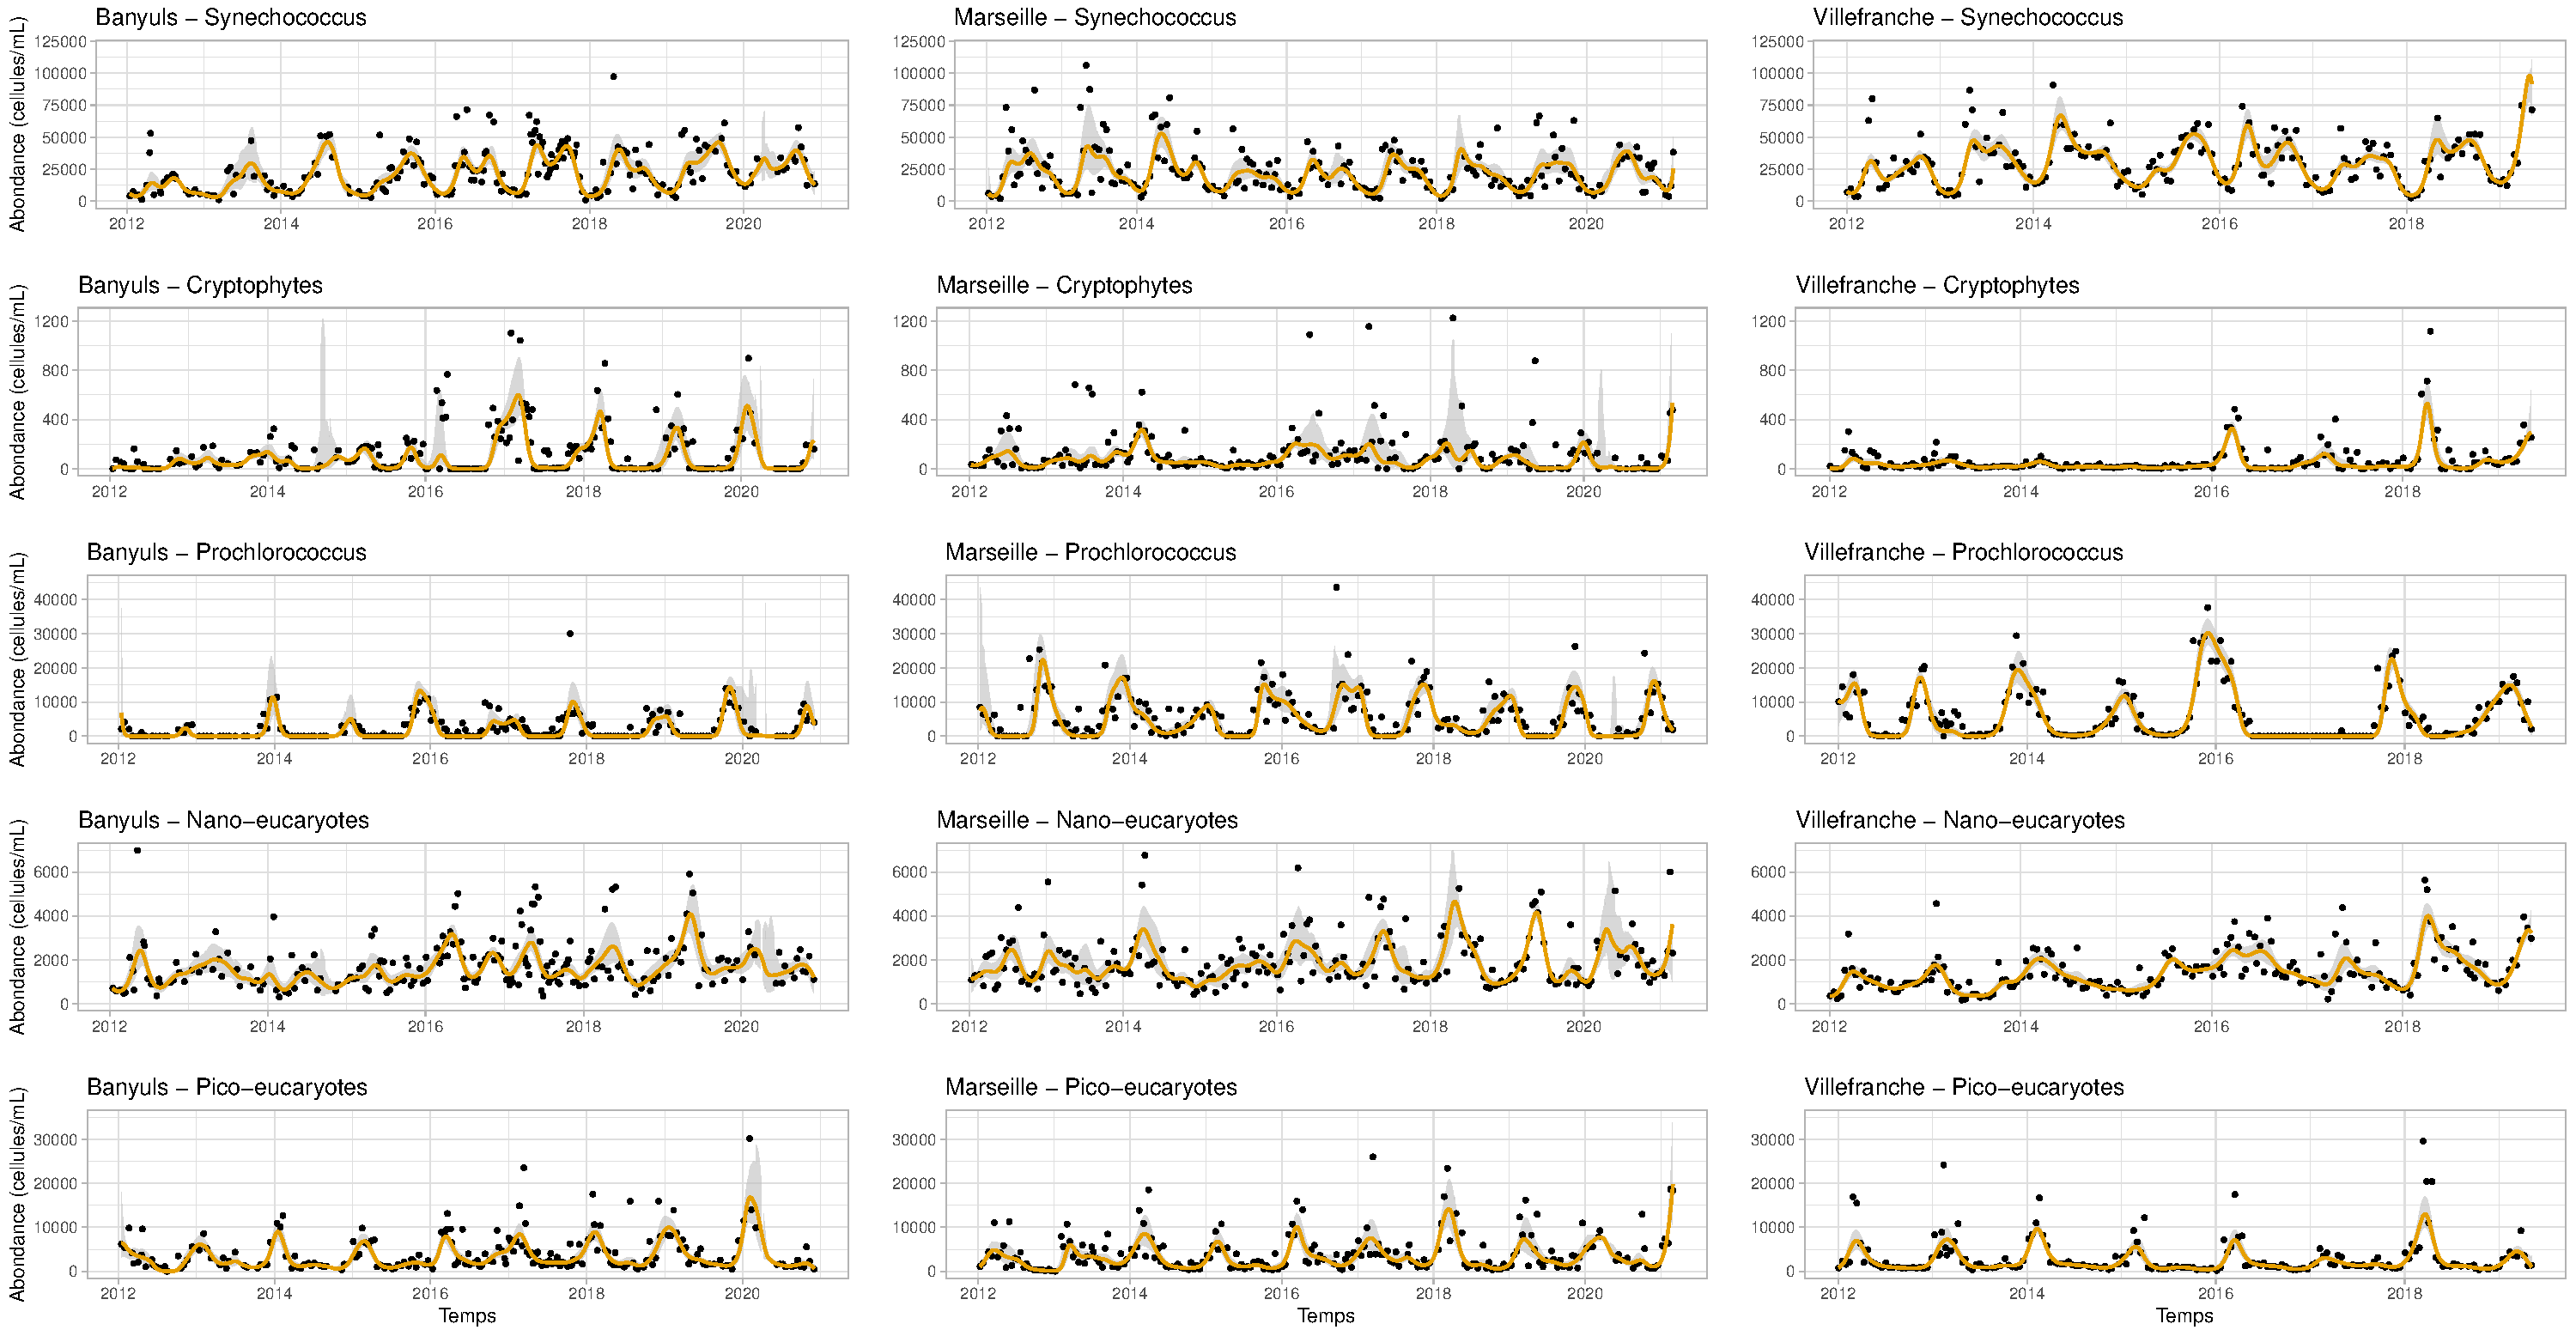
\includegraphics[width=\textheight]{fig/R11_ts_ab.pdf}
\caption{Séries temporelles des abondances des groupes de phytoplancton pour les trois stations méditerranéennes. Les points noirs correspondent aux données brutes, la courbe orange à la régression quadratique locale avec noyau gaussien avec une fenêtre de 40 jours. Elle est associée à son intervalle de confiance à 95\% en gris.}
\label{ts_ab}
\end{sidewaysfigure}

Pour caractériser la saisonnalité, le périodogramme de chaque régression est réalisé. Le périodogramme des \textit{Synechococcus} à Banyuls est présenté en Figure \ref{period}. Celui-ci identifie clairement deux maxima à des fréquences de 1.02$\Delta$ et 2$\Delta$. Le pic à la fréquence 1.02$\Delta$ correspond environ à 1 cycle par an, soit une saisonnalité annuelle. Le pic à la fréquence 2$\Delta$ correspond à 2 cycles par an, soit une saisonnalité de 6 mois. Les bornes inférieures de l’intervalle de confiance à 95\% des deux pics sont supérieures au reste du signal. Ils peuvent donc être considérés comme significatifs. En revanche, la petite bosse qui ressort à une fréquence de 2.97$\Delta$ n’est pas significative. Pour les autres séries, à l’exception des nano-eucaryotes à Villefranche, les périodogrammes permettent de mettre en évidence une saisonnalité annuelle significative. Les nano-eucaryotes à Villefranche présentent des cycles de 2 ans. Pour les pico-eucaryotes et les \textit{Synechococcus} aux trois stations, et pour les nano-eucaryotes à Banyuls, une saisonnalité significative de 6 mois est aussi mise en évidence.  

\begin{figure}
\centering
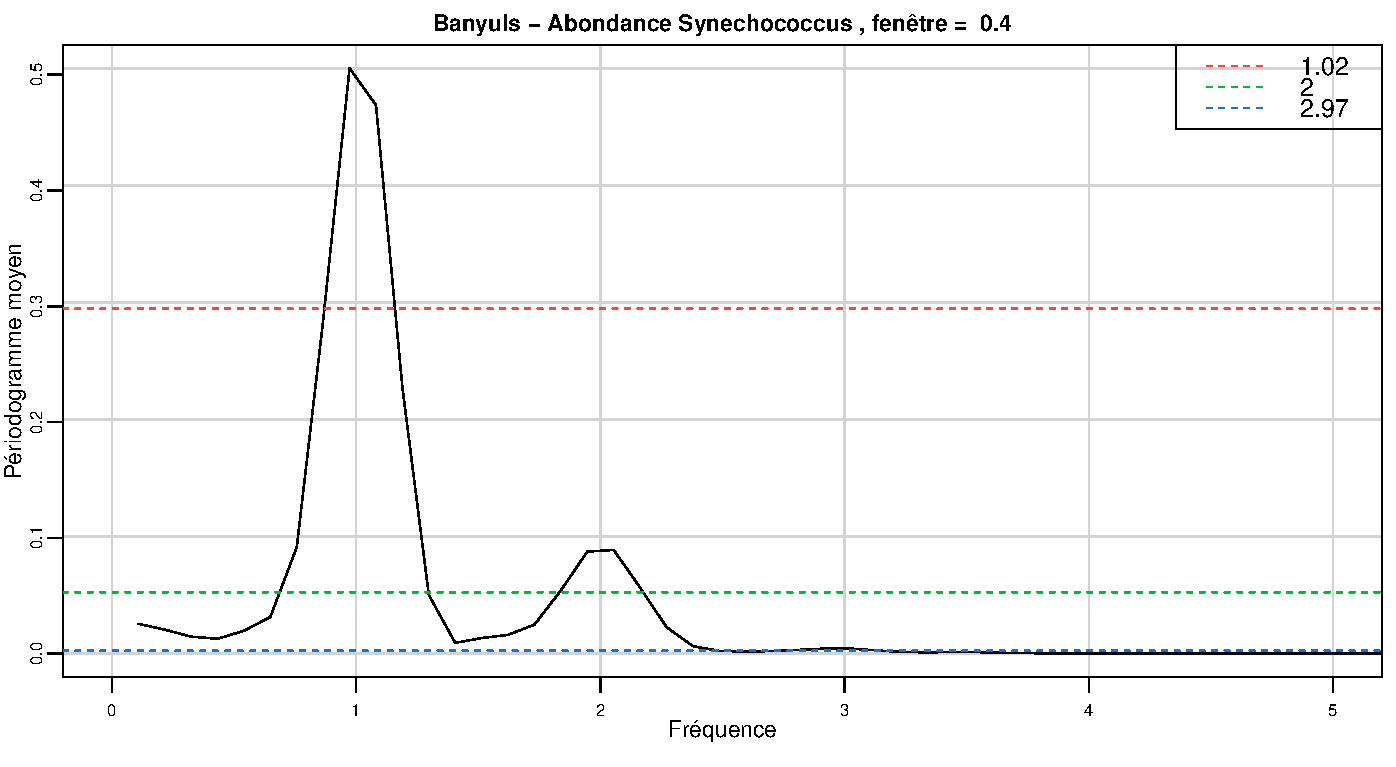
\includegraphics[width=.7\textwidth]{fig/R12_period_syn_banyuls.pdf}
\caption{Périodogramme moyen de la série d'abon\-dance de \textit{Synechococcus} à Banyuls. L'axe de fréquences est gradué par multiple de $\Delta=1 cycle/1 an$. Les lignes pointillées correspondent à la borne inférieure de l'intervalle de confiance à 95\% des pics identifiés dans la légende.}
\label{period}
\end{figure}


\subsubsection{Température}

Dans le contexte du réchauffement climatique, nous cherchons d’abord à voir comment il se fait ressentir au sein des stations. Une des analyse qui a été réalisée se focalise sur l'évolution au cours du temps de la température de la colonne d'eau à Marseille. 

Les données CTD des profils de température à Marseille ne sont pas observées à intervalle de profondeur régulier. Il y a environ une observation tous les 0,2 ou 0,3m. Une interpolation est réalisée pour avoir des données régulières tous les 0,5m de 0,5m à 55m de profondeur. Ce qui représente 112 points pour chaque profils verticaux. Le choix est fait de prendre deux fois moins de fonctions de bases que de points. Pour obtenir un profil lisse qui ne présente pas trop d'ondulations, un lissage avec pénalisation de la courbure avec 55 fonctions de bases est réalisé. Plusieurs paramètres de lissage $\lambda$ sont testés et le lissage obtenu avec chaque paramètre est visualisé pour 8 profils choisis au hasard. Nous faisons le choix de conserver $\lambda = 0.1$ qui produit le lissage visualisé en Figure \ref{lambda_ctd}. 

\begin{figure}
\centering
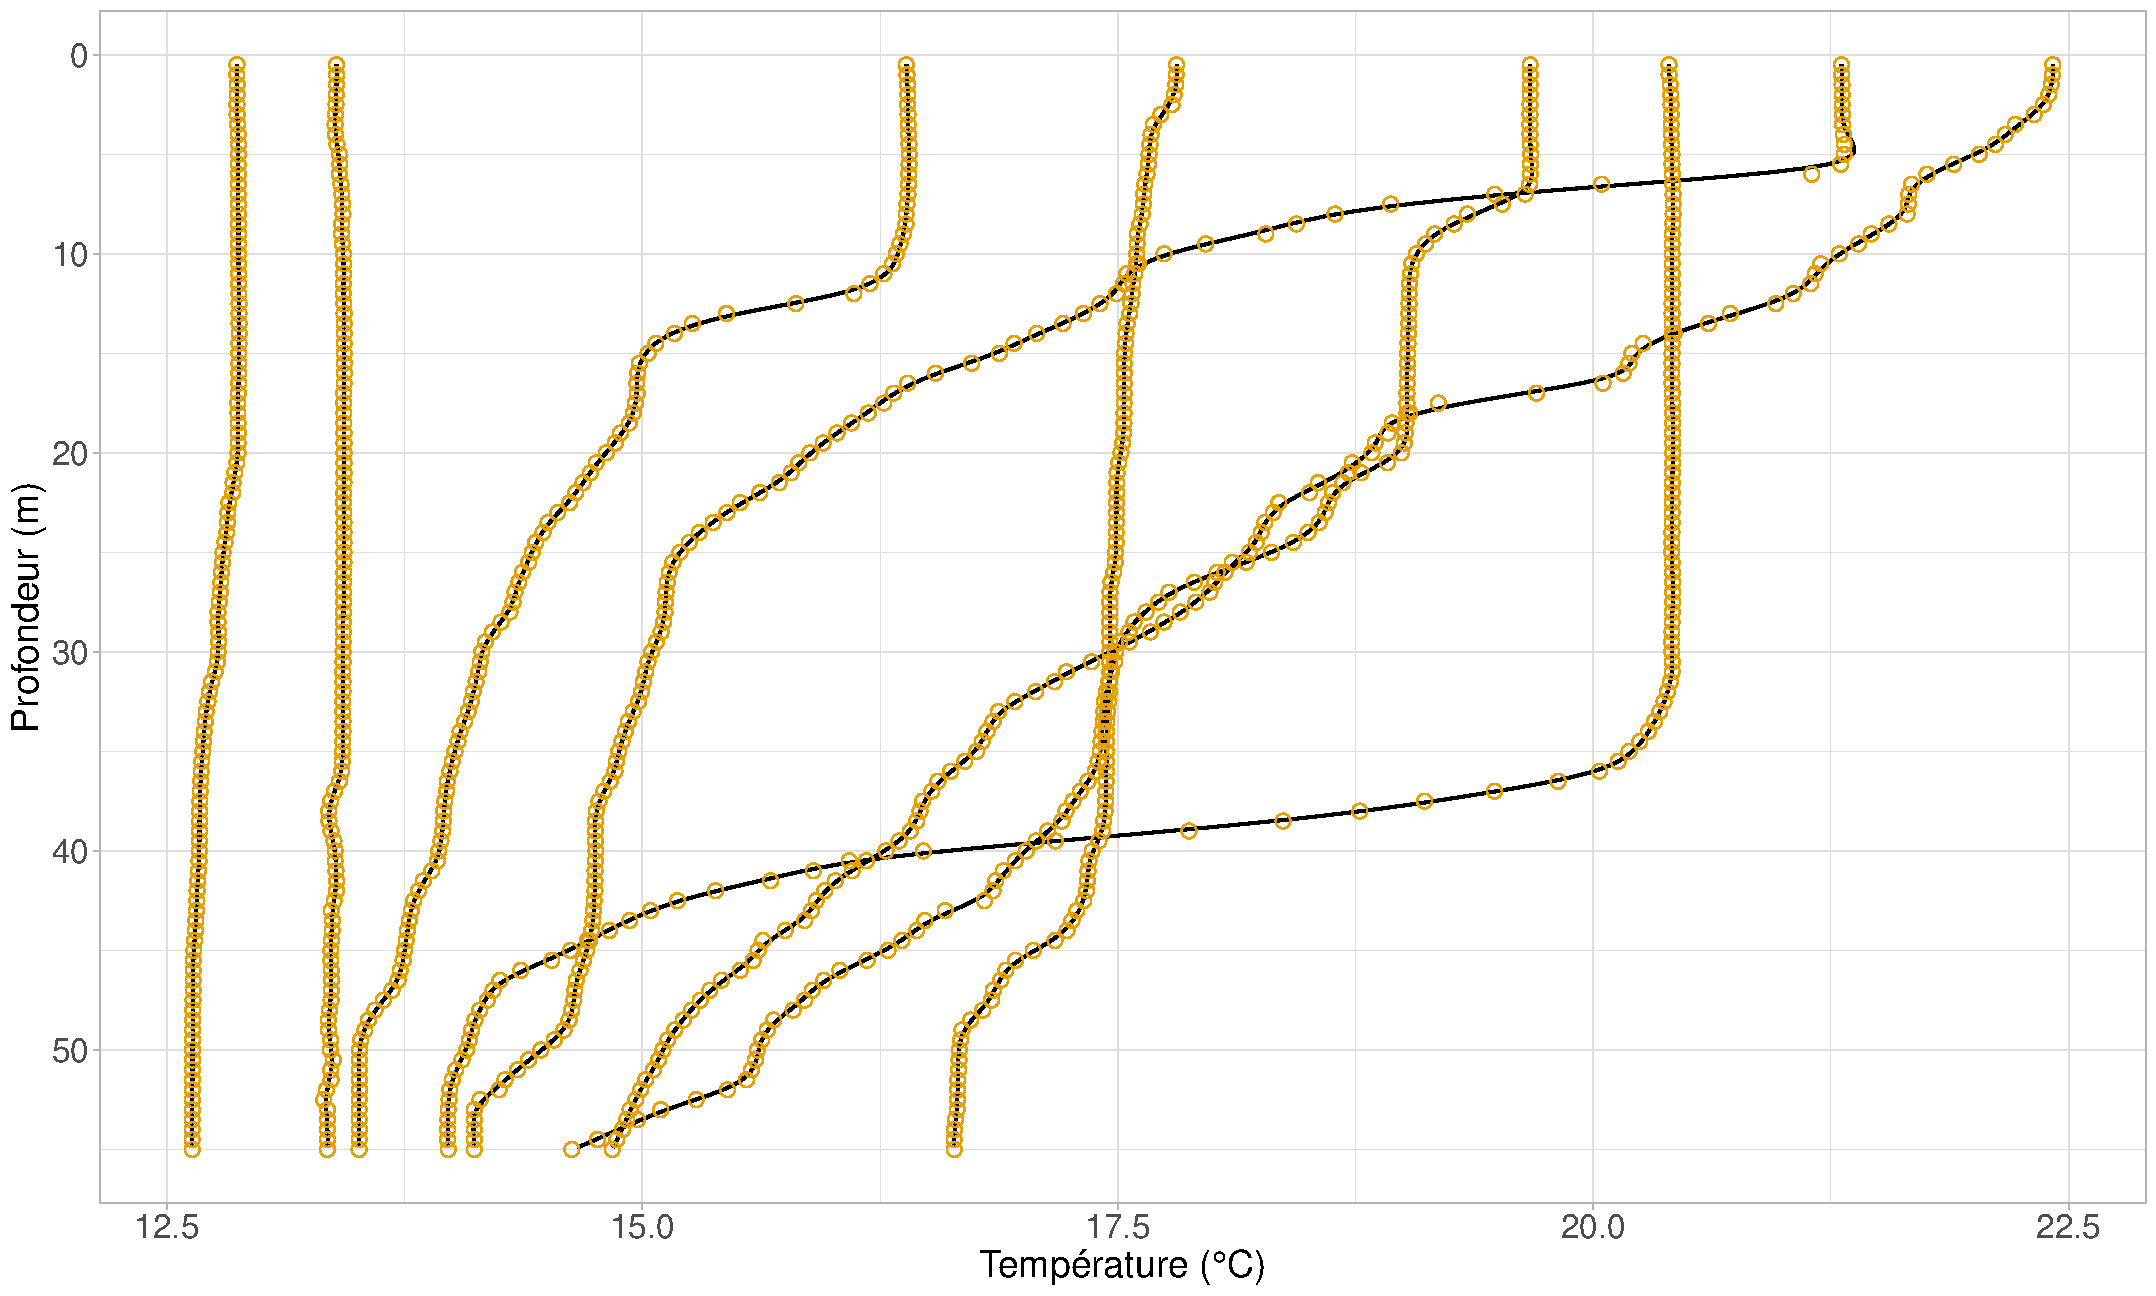
\includegraphics[width=.75\textwidth]{fig/R131_prof_lambda.pdf}
\caption{Profils verticaux de température à Marseille après lissage avec pénalisation, $\lambda=0,1$, à partir des points oranges pour 8 dates choisies au hasard.}
\label{lambda_ctd}
\end{figure}

À partir des courbes lissées, l’ACP fonctionnelle est réalisée sur tous les profils de température à Marseille.  Les deux premières composantes principales de cette ACP résument à elles deux 97,78\% des variations observées entre toutes les courbes. L’effet de ces deux premières composantes est présenté sur la Figure \ref{acp_ctd}a). Un écart positif à la moyenne, représentée par la courbe noire, signifie que le profil se rapproche de la courbe représentée par des croix grises. Un écart négatif à la moyenne signifie que le profil se rapproche de la courbe représentée par des tirets oranges. Sur une visualisation bi-dimensionnelle des scores de l’ACP, cette moyenne correspondrait à l’origine des axes. La première composante principale (PC1), qui représente 89,7\% des variations, représente un effet moyen. Une valeur positive sur l’axe 1 indique que la température moyenne du profil est supérieure à la moyenne de tous les profils. À l’inverse, une valeur négative sur l’axe 1 implique que la température moyenne du profil lui est inférieure. La deuxième composante principale (PC2), qui représente 8,08\% des variations, représente un effet de stratification. Une valeur positive sur l’axe 2 implique que la température est plutôt homogène le long de la colonne d’eau. Une valeur négative sur l’axe 2 suggère une forte diminution de la température à mesure que la profondeur augmente. La Figure \ref{acp_ctd} b) représente sous forme de séries temporelles les scores des deux premières composantes principales pour chaque profil CTD observé. Une saisonnalité annuelle est observable pour les deux composantes. La PC1 met en évidence une température moyenne plus basse la première partie de l’année. La PC2 quant à elle met en évidence une forte stratification de la colonne d’eau en milieu d’année. À partir de 2003 cette stratification semble plus importante puisque des valeurs négatives plus extrêmes sot observées. 



\begin{figure}
\centering
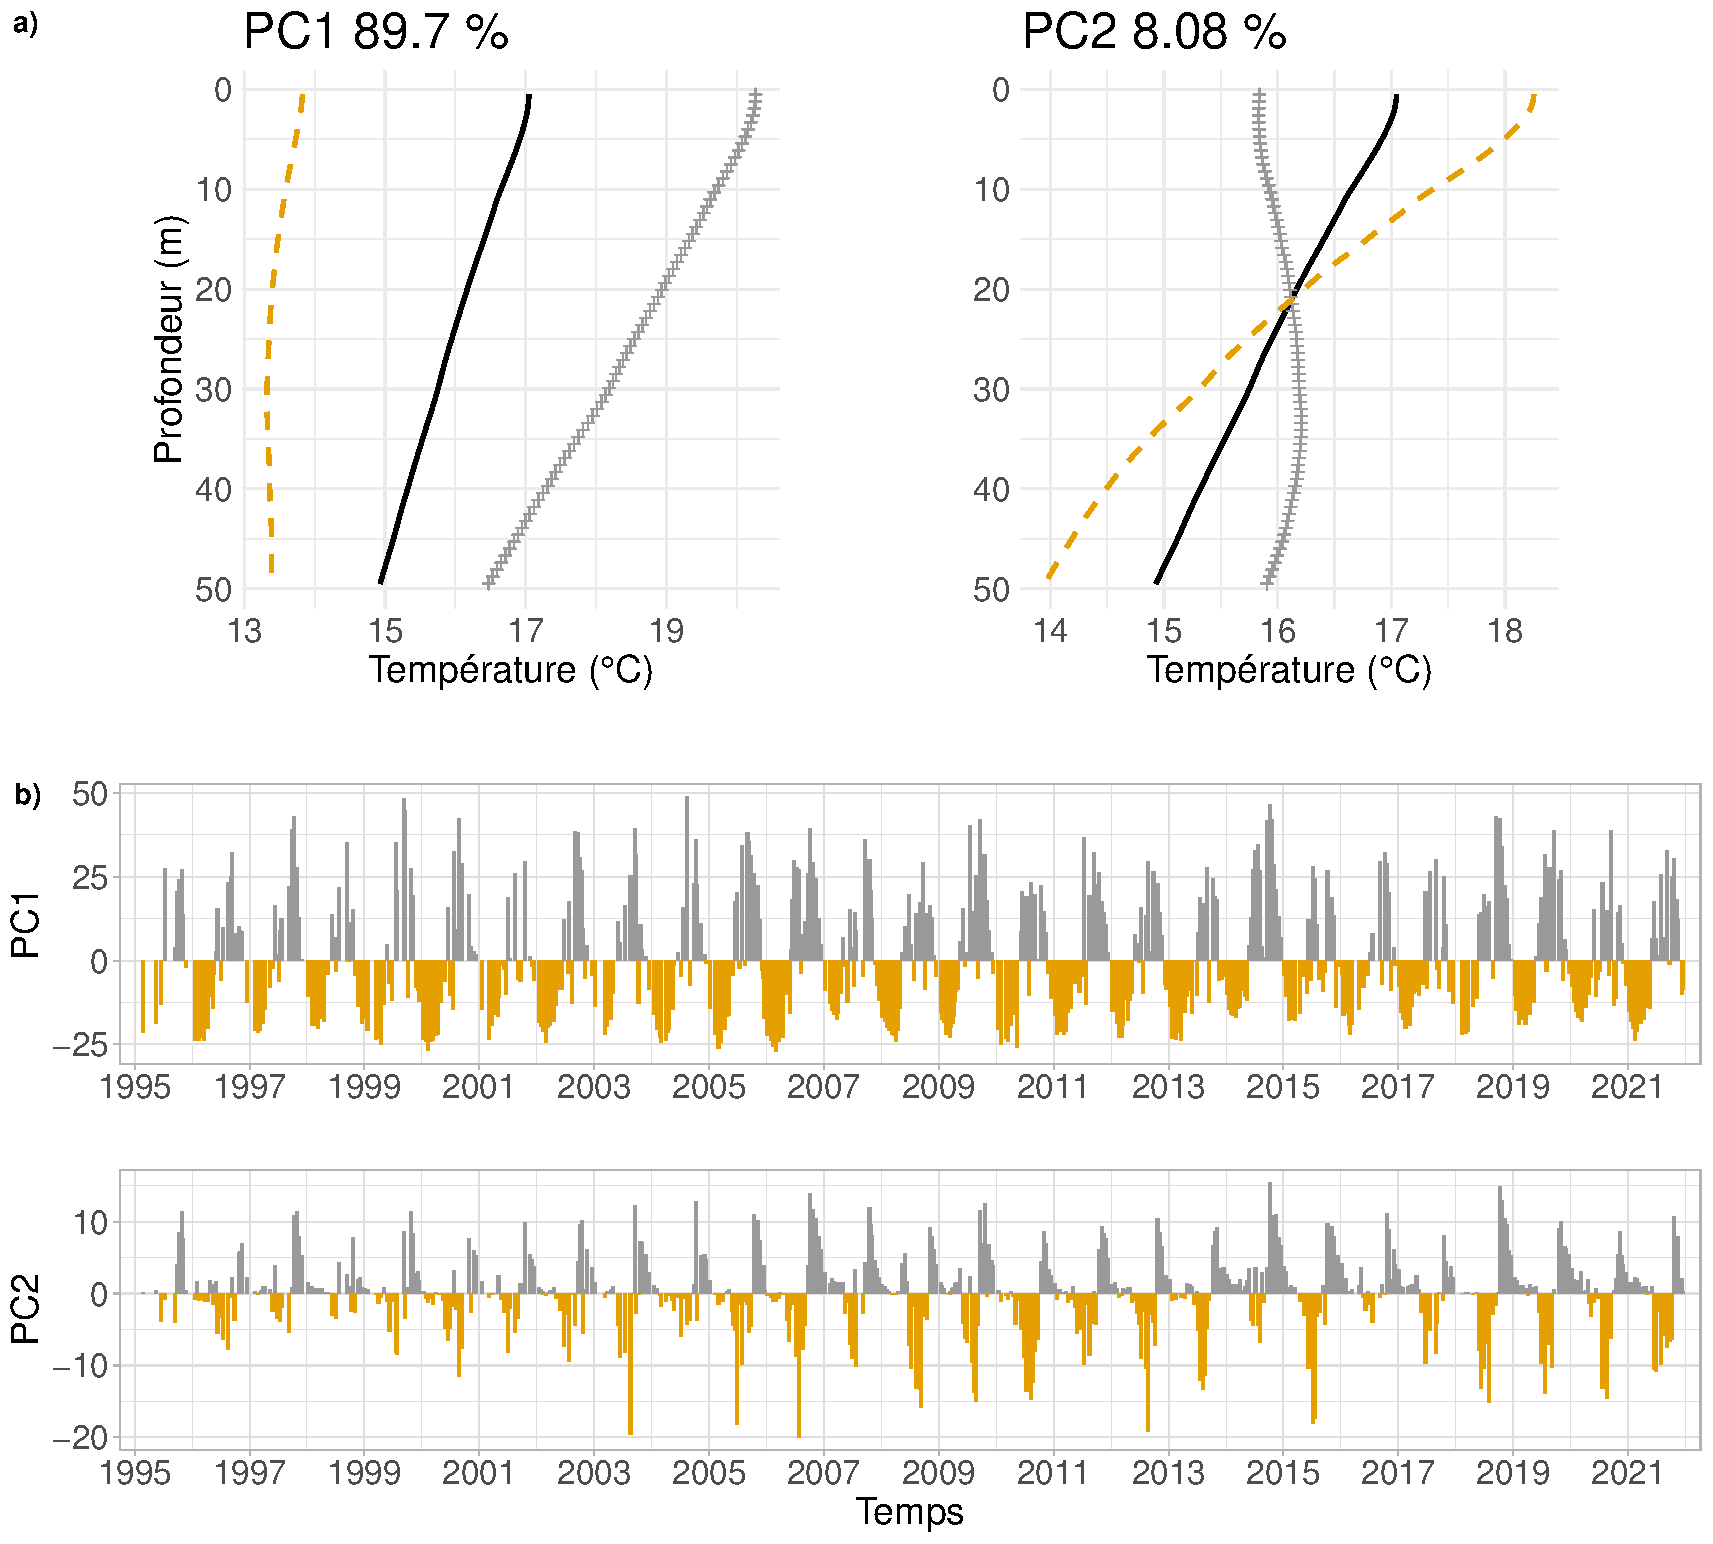
\includegraphics[width=.9\textwidth]{fig/R132_mean_pert_CTD.pdf}
\caption{a) Deux premières composantes principales de l'ACP fonctionnelle des profils de température à Marseille, exprimées comme perturbation de la moyenne. La courbe noire correspond au profil moyen. En croix grises est représenté l’effet d’une perturbation positive et en tirets orange est représenté l’effet d’une perturbation négative. b) Séries temporelles des scores des deux premières composantes principales.
}
\label{acp_ctd}
\end{figure}

Une manière de comparer les années entres-elles est de réaliser une ACP fonctionnelle sur les unités annuelles de chaque composante principale. Les séries temporelles des scores des PC1 et PC2 de l’ACP fonctionnelle précédente sont utilisées. Les ACP fonctionnelles sont réalisées séparément pour les deux composantes. Pour chaque ACP, une fonction correspond à l’évolution du score de la composante sur une année. Les dates d’observations correspondent aux mêmes dates d’échantillonnage des profils CTD. Pour avoir des observations régulières, une moyenne mensuelle des scores pour chaque année est réalisée, ce qui représente donc 12 observations par an. Comme pour plusieurs années, certains mois ne comportent aucune observation, nous utilisons alors le paquet $fdapace$ qui permet de combler ces lacunes pour conserver le plus grand nombre d’années dans la comparaison

La Figure \ref{acp_pc} présente les résultats de l’ACP fonctionnelle sur la deuxième composante principale des profils verticaux. Rappelons qu’elle représente l’évolution de la stratification de la colonne d’eau au cours d’une année. La courbe moyenne en noire indique qu’on observe une forte stratification de la colonne d’eau en été, exprimée par des valeurs négatives du PC2.  Au contraire, à la fin de l’année, la température de la colonne d’eau est plutôt homogène puisque les valeurs du PC2 sont positives. %Maintenant, si l’on regarde l’effet des composantes principales de la dernière ACP, on voit que%
Les deux premières composantes résument 88,63\% des variations observées entre chaque année, de 1994 à 2021. La première composante principale représente 73,71\% de ces variations. Elle illustre une différence dans la magnitude, en même temps qu’un décalage dans le temps de la stratification. La deuxième composante principale, qui constitue 14,92\% des variations, rend compte d’un effet moyen.  La visualisation des scores de l’ACP sur deux dimensions montre que les premières années de la série sont plutôt regroupées dans le cadran inférieur gauche alors que les années les plus récentes se situent plutôt dans le cadran supérieur droit. 

\begin{figure}
\centering
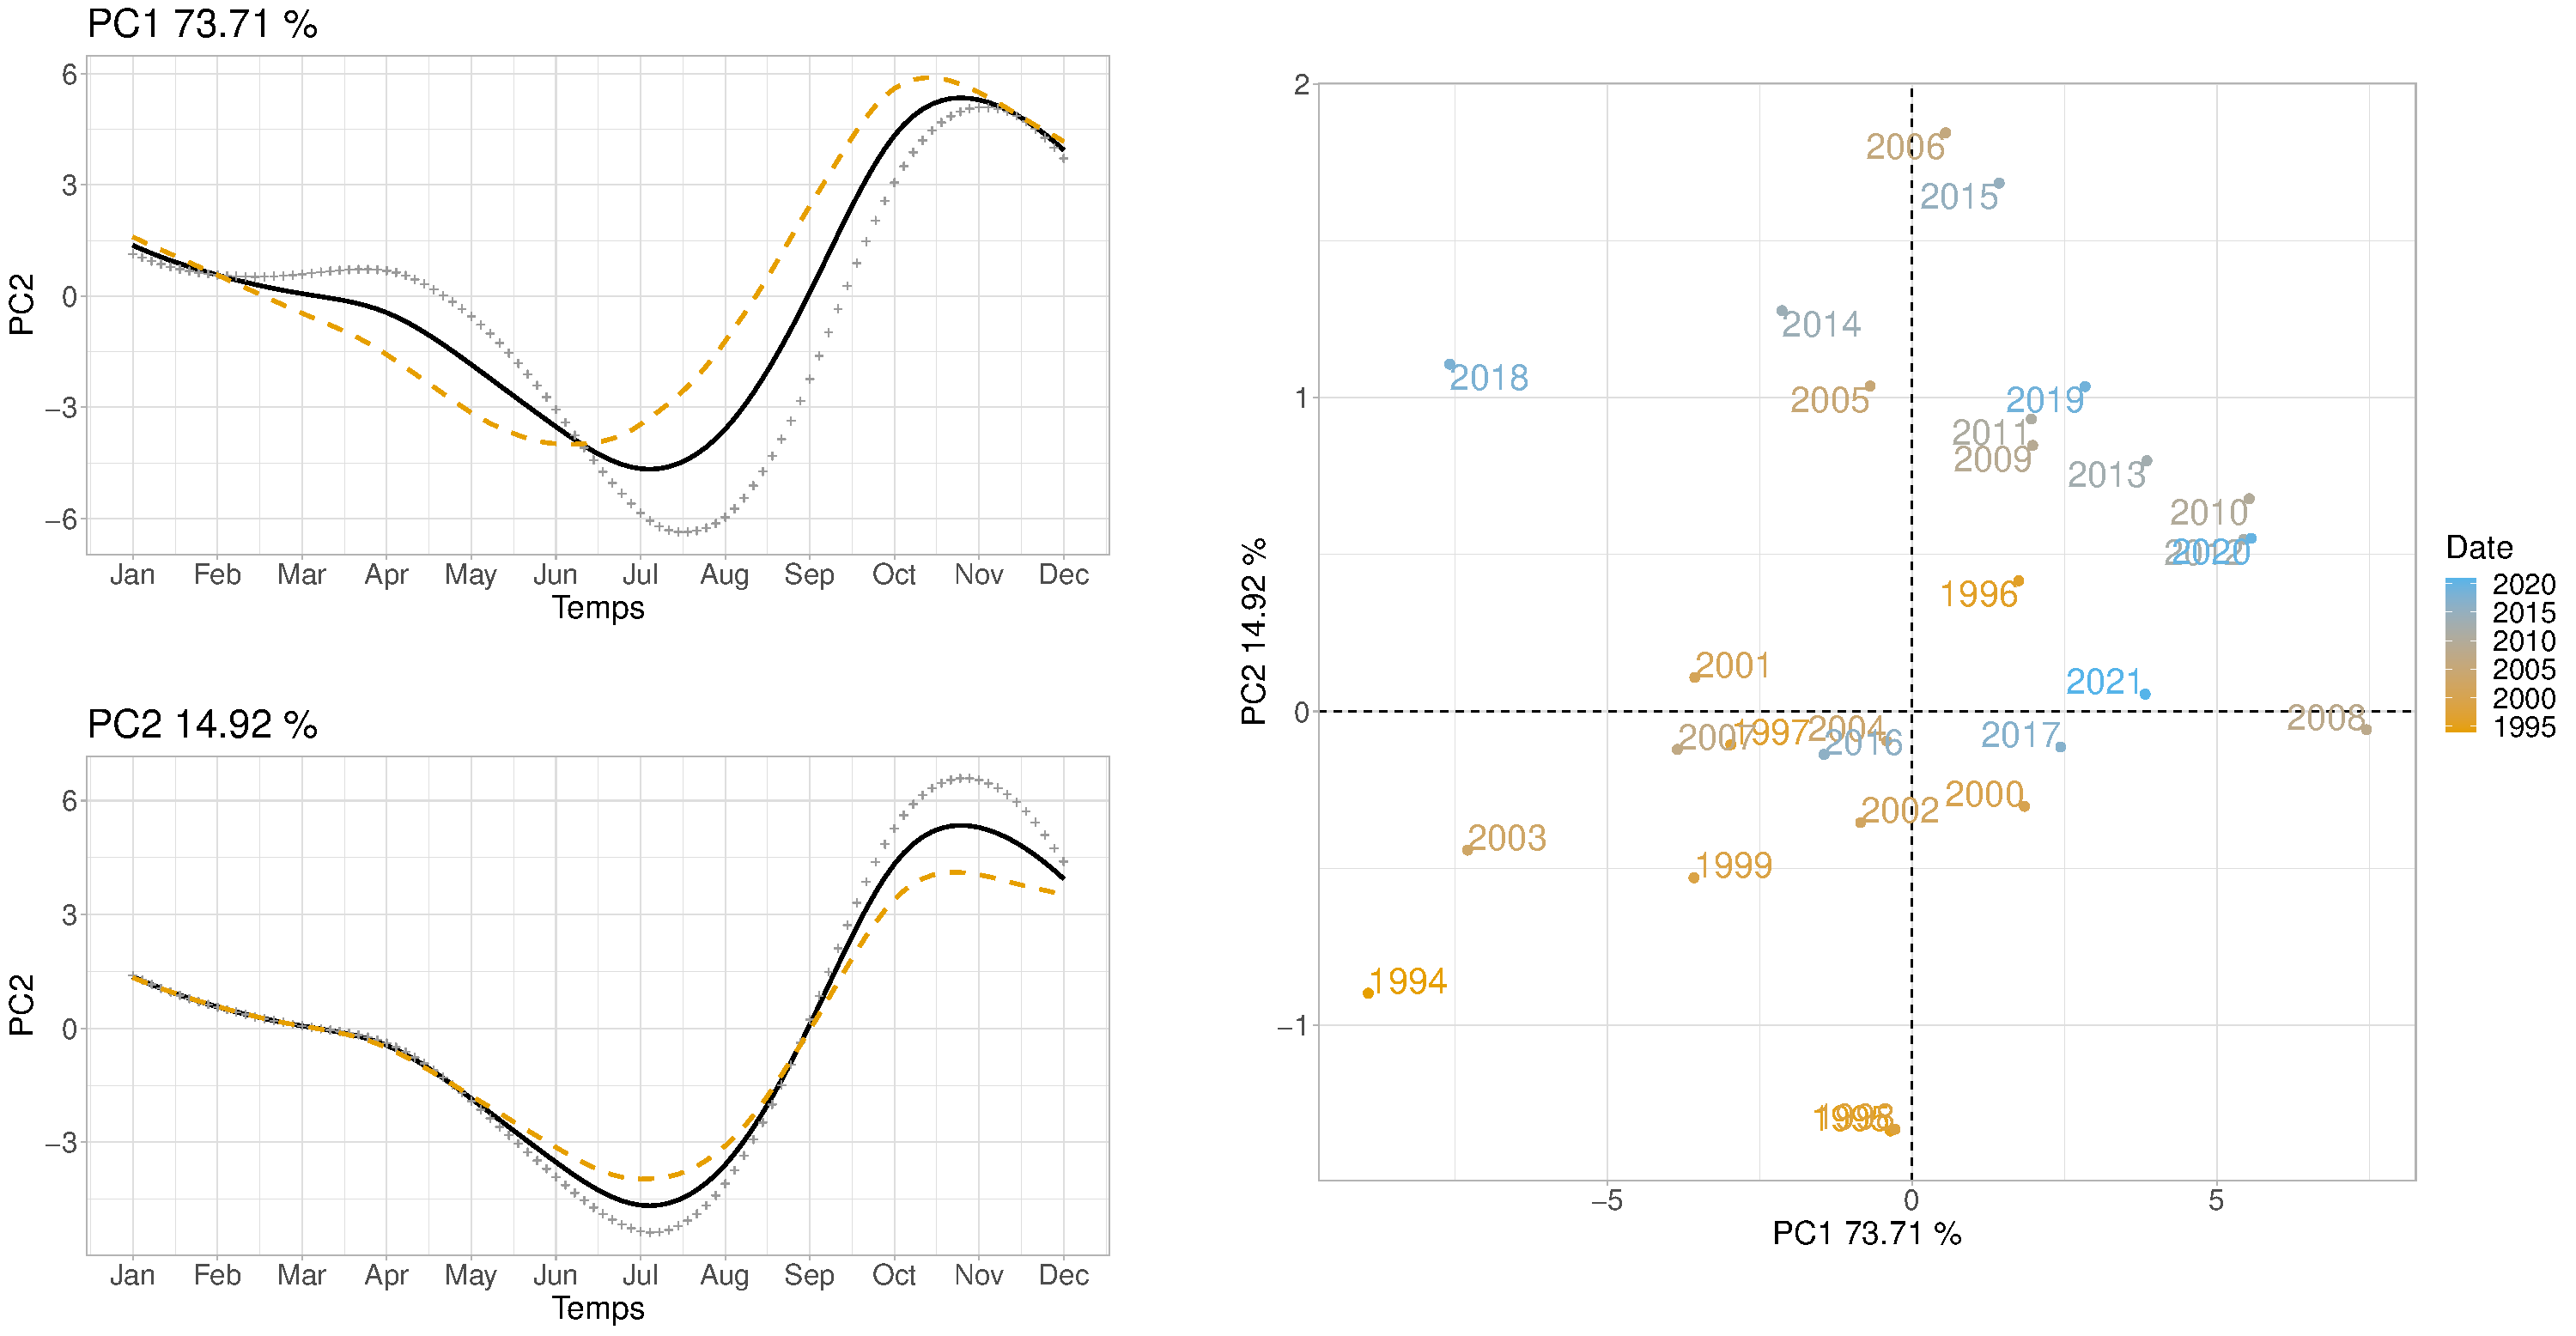
\includegraphics[width=.9\textwidth]{fig/R133_ACP_PC.pdf}
\caption{(gauche) Deux premières composantes principales de l'ACP fonctionnelle de la PC2 des profils verticaux de température à Marseille, exprimées comme perturbation de la moyenne. La courbe noire correspond au profil moyen. En croix grises est représenté l’effet d’une perturbation positive et en tirets orange est représenté l’effet d’une perturbation négative. (droite) Score des deux premières composantes principales.}
\label{acp_pc}
\end{figure}

\subsection{Variations dans l'espace}

Nous cherchons maintenant à distinguer les stations en fonction de l’évolution de chaque variable au cours de l’année. Nous nous intéressons ici aussi, à des unités annuelles. 

\subsubsection{Abondance des groupes phytoplanctoniques}

Pour savoir si les stations se distinguent en terme d'abondance de chaque groupe de phytoplancton au cours de l'année, nous nous intéressons tout d'abord aux données d'abondance. 

Pour chaque groupe de phytoplancton toutes stations confondues, une ACP fonctionnelle est réalisée sur les données d’abondance. Comme il y a 5 groupes, nous allons donc effectuer 5 ACP différentes. Ici, une fonction correspond à l’évolution de l’abondance d'un groupe à une station, sur un an. Pour avoir des observations régulières, une moyenne mensuelle des données échantillonnées est réalisée pour chaque année. Il y a donc 12 points par an. Pour pouvoir conserver le plus grand nombre d’années dans la comparaison, le paquet $fdapace$ est utilisé. Les deux premières composantes des ACP sont présentées en Annexe A sous forme de perturbations de la moyenne. L’effet de toutes les premières composantes principales est un effet moyen où des valeurs positives impliquent une augmentation et des valeurs négatives une diminution. L’inertie des deuxièmes composantes principales des ACP sur les abondances varie entre 8,7\% à 25,8\%. Ces deuxièmes composantes principales sont conservées pour l’AFD.

Nous obtenons un nouveau tableau d’observations. Chaque observation correspond à une année, avec une variable qualitative qui correspond au site et 10 variables quantitatives qui correspondent aux scores des deux premières composantes principales des ACP pour chaque groupe de phytoplancton. 

Les résultats de l’AFD sur ce tableau est présenté en Figure \ref{afd_ab}. Les résultats de l’AFD sur ce tableau est présenté en Figure \ref{afd_ab}. Les deux axes résument bien 100\% des informations. Le premier est celui qui contribue le plus à la discrimination, à hauteur de 94,94\%. Le deuxième axe a donc une contribution de 5,06\%. Le premier axe permet une bonne discrimination des sites de Banyuls et Marseille. Le deuxième axe quant à lui, discrimine très bien le site de Villefranche des deux autres. 


\begin{figure}
\centering
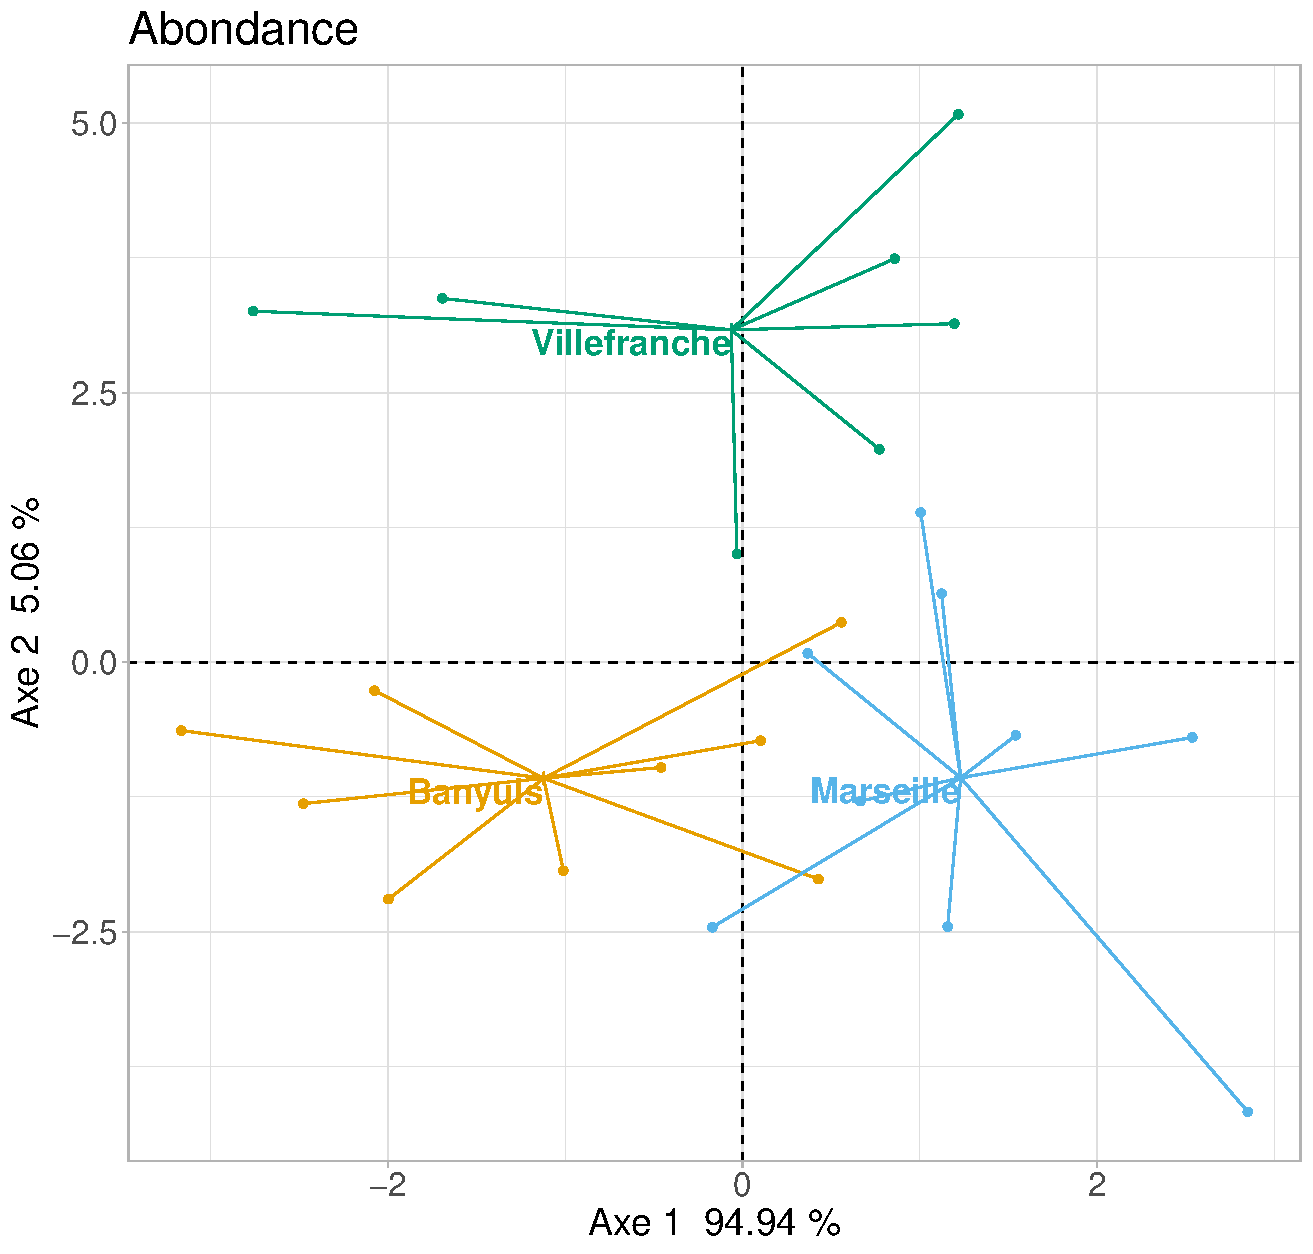
\includegraphics[width=.65\textwidth]{fig/R221_FDA_ab.pdf}
\caption{Graphique des individus de l'AFD des unités annuelles d'abondance des groupes de phytoplancton pour les trois stations SOMLIT méditerranéennes.}
\label{afd_ab}
\end{figure}

La Figure \ref{afd_ab_var} correspond au graphique des corrélations des variables associées à l’AFD. Les PC1 correspondent à l’abondance moyenne de chaque groupe. Les PC2 sont illustrées sur les bords de la Figure \ref{afd_ab_var}. Le PC1 des \textit{Prochlorococcus} est celui contribue le plus à l’axe 1. Cela signifie que l’abondance des \textit{Prochlorococcus} est supérieure à Marseille de janvier à septembre (Annexe A).  Les variables qui contribuent le plus à l’axe 2 sont les PC2 des nano-eucaryotes et des \textit{Prochlorococcus}. Cela indique d’une part, qu’à Villefranche l’abondance des nano-eucaryotes atteint un maximum plus importante de janvier à mai et diminue fortement le reste de l’année. À Banyuls et à Marseille, ce pic est moins important et l’abondance diminue moins le reste de l’année. D’autre part, à Villefranche l’abondance des \textit{Prochlorococcus} est moins importante en début d’année, mais diminue moins en été qu’aux deux autres stations.

\begin{figure}
\centering
\hspace*{-35pt}
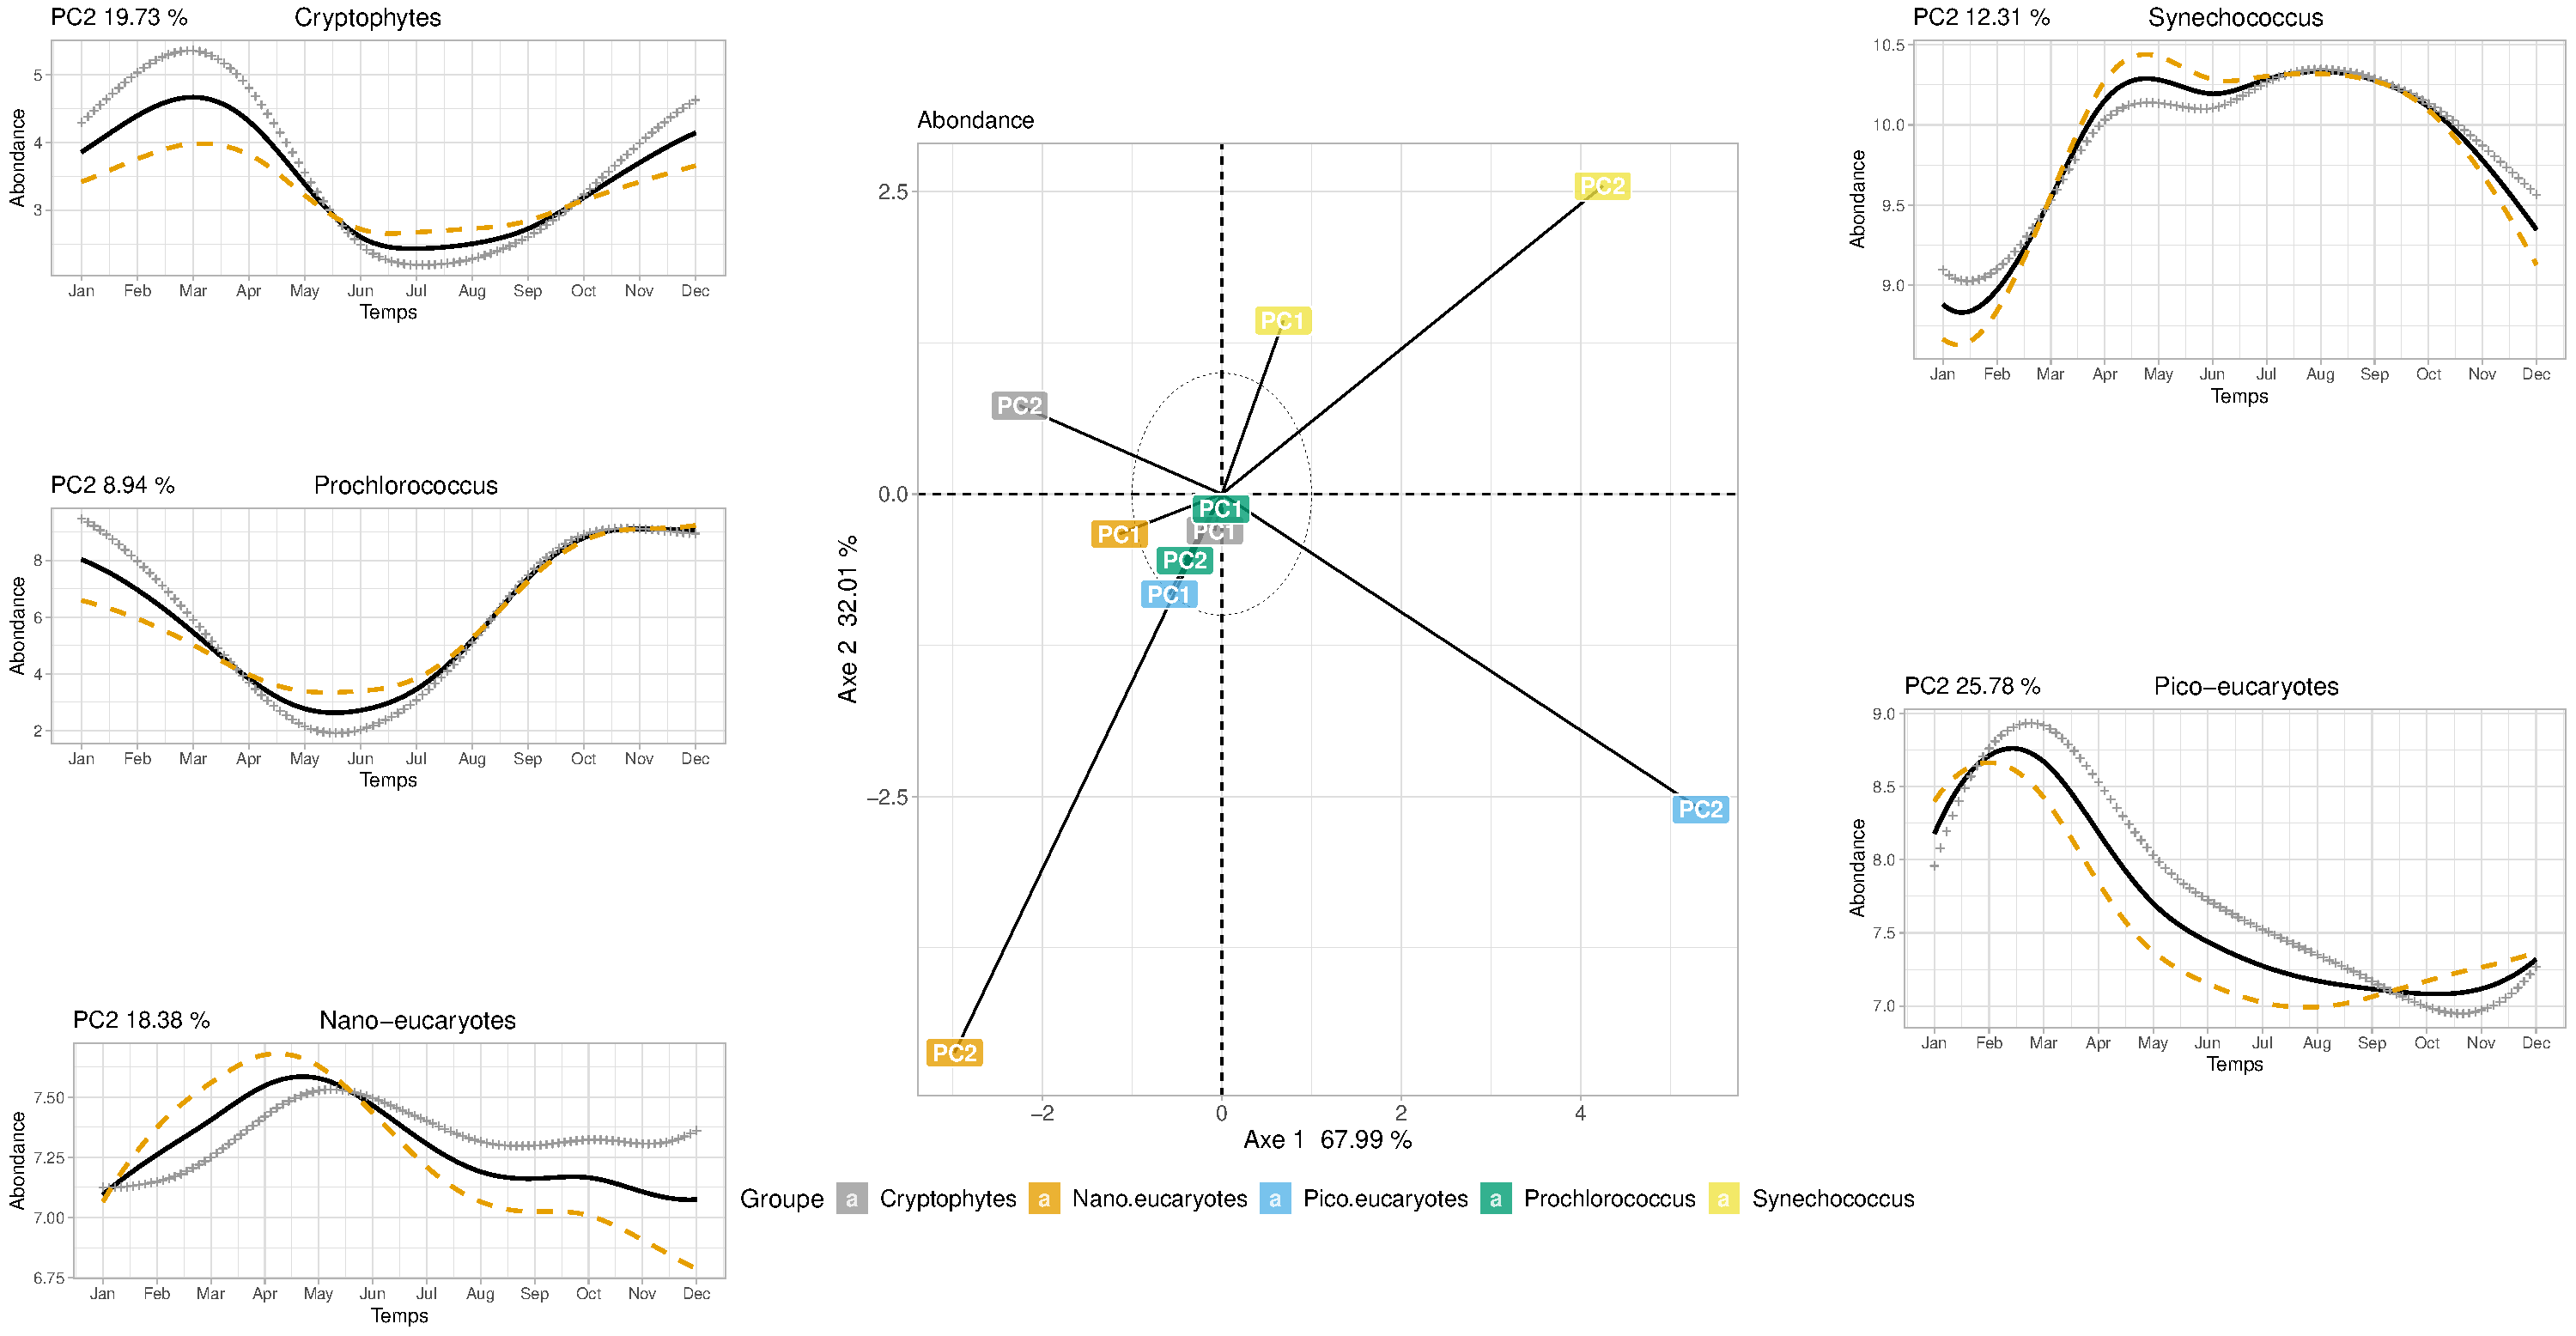
\includegraphics[width=1.1\textwidth]{fig/R222_fda_fpca_ab.pdf}
\caption{(centre) Graphique des corrélations des variables de l'AFD des unités annuelles d'abondance des groupes de phytoplancton pour les trois stations SOMLIT méditer\-ranéennes. (côtés) Deuxièmes composantes principales des ACP fonctionnelles d'abondance du phytoplancton exprimées comme perturbation de la moyenne. La courbe noire correspond au profil moyen. En croix grises est représenté l’effet d’une perturbation positive et en tirets orange est représenté l’effet d’une perturbation négative.}
\label{afd_ab_var}
\end{figure}

\subsubsection{Diffusion lumineuse des groupes phytoplanctoniques}

Nous voulons voir si les sites se distinguent par des populations présentant des organismes de taille différente. 

Comme pour l’abondance, une ACP est réalisée pour chaque groupe de phytoplancton toutes stations confondues, avec les données de diffusion lumineuse. Les deux premières composantes des ACP sont présentées en Annexe C sous forme de perturbations de la moyenne. L’effet de toutes les premières composantes principales est un effet moyen où des valeurs positives impliquent une augmentation et des valeurs négatives impliquent une diminution. L’inertie des deuxièmes composantes principales des ACP est majoritairement inférieure à 10\%. Nous choisissons de ne pas conserver ces deuxièmes composantes principales pour l’AFD.

On obtient un nouveau tableau d’observations. Chaque observation correspond à une année, avec une variable qualitative qui correspond au site et 5 variables quantitatives qui correspondent aux scores de la première composante principale des ACP pour chaque groupe du phytoplancton. 

Les résultats de l’AFD sur ce tableau est présenté en Figure \ref{afd_ab}. Les deux axes résument bien 100\% des informations. Le premier est celui qui contribue le plus à la discrimination, à hauteur de 90,18\%. Le deuxième axe a donc une contribution de 9,82\%. L’association des deux axes permet une bonne discrimination entre Banyuls et les deux autres sites. Cependant les sites de Marseille et Villefranche ne se distinguent pas très bien. En ce qui concerne la corrélation des variables, une forte SSC des nano-eucaryotes s’oppose à une forte SSC des \textit{Synechococcus} et des pico-eucaryotes. Le PC1 des \textit{Prochlorococcus} est celui qui semble contribuer le plus à l’axe 2. À Banyuls les nano-eucaryotes ont des valeurs de SSC plus importantes toute l’année, mais des \textit{Prochlorococcus}, des \textit{Synechococcus} et des pico-eucaryotes avec des valeurs de SSC plus faibles toute l’année (Annexe C). 



\begin{figure}
\centering
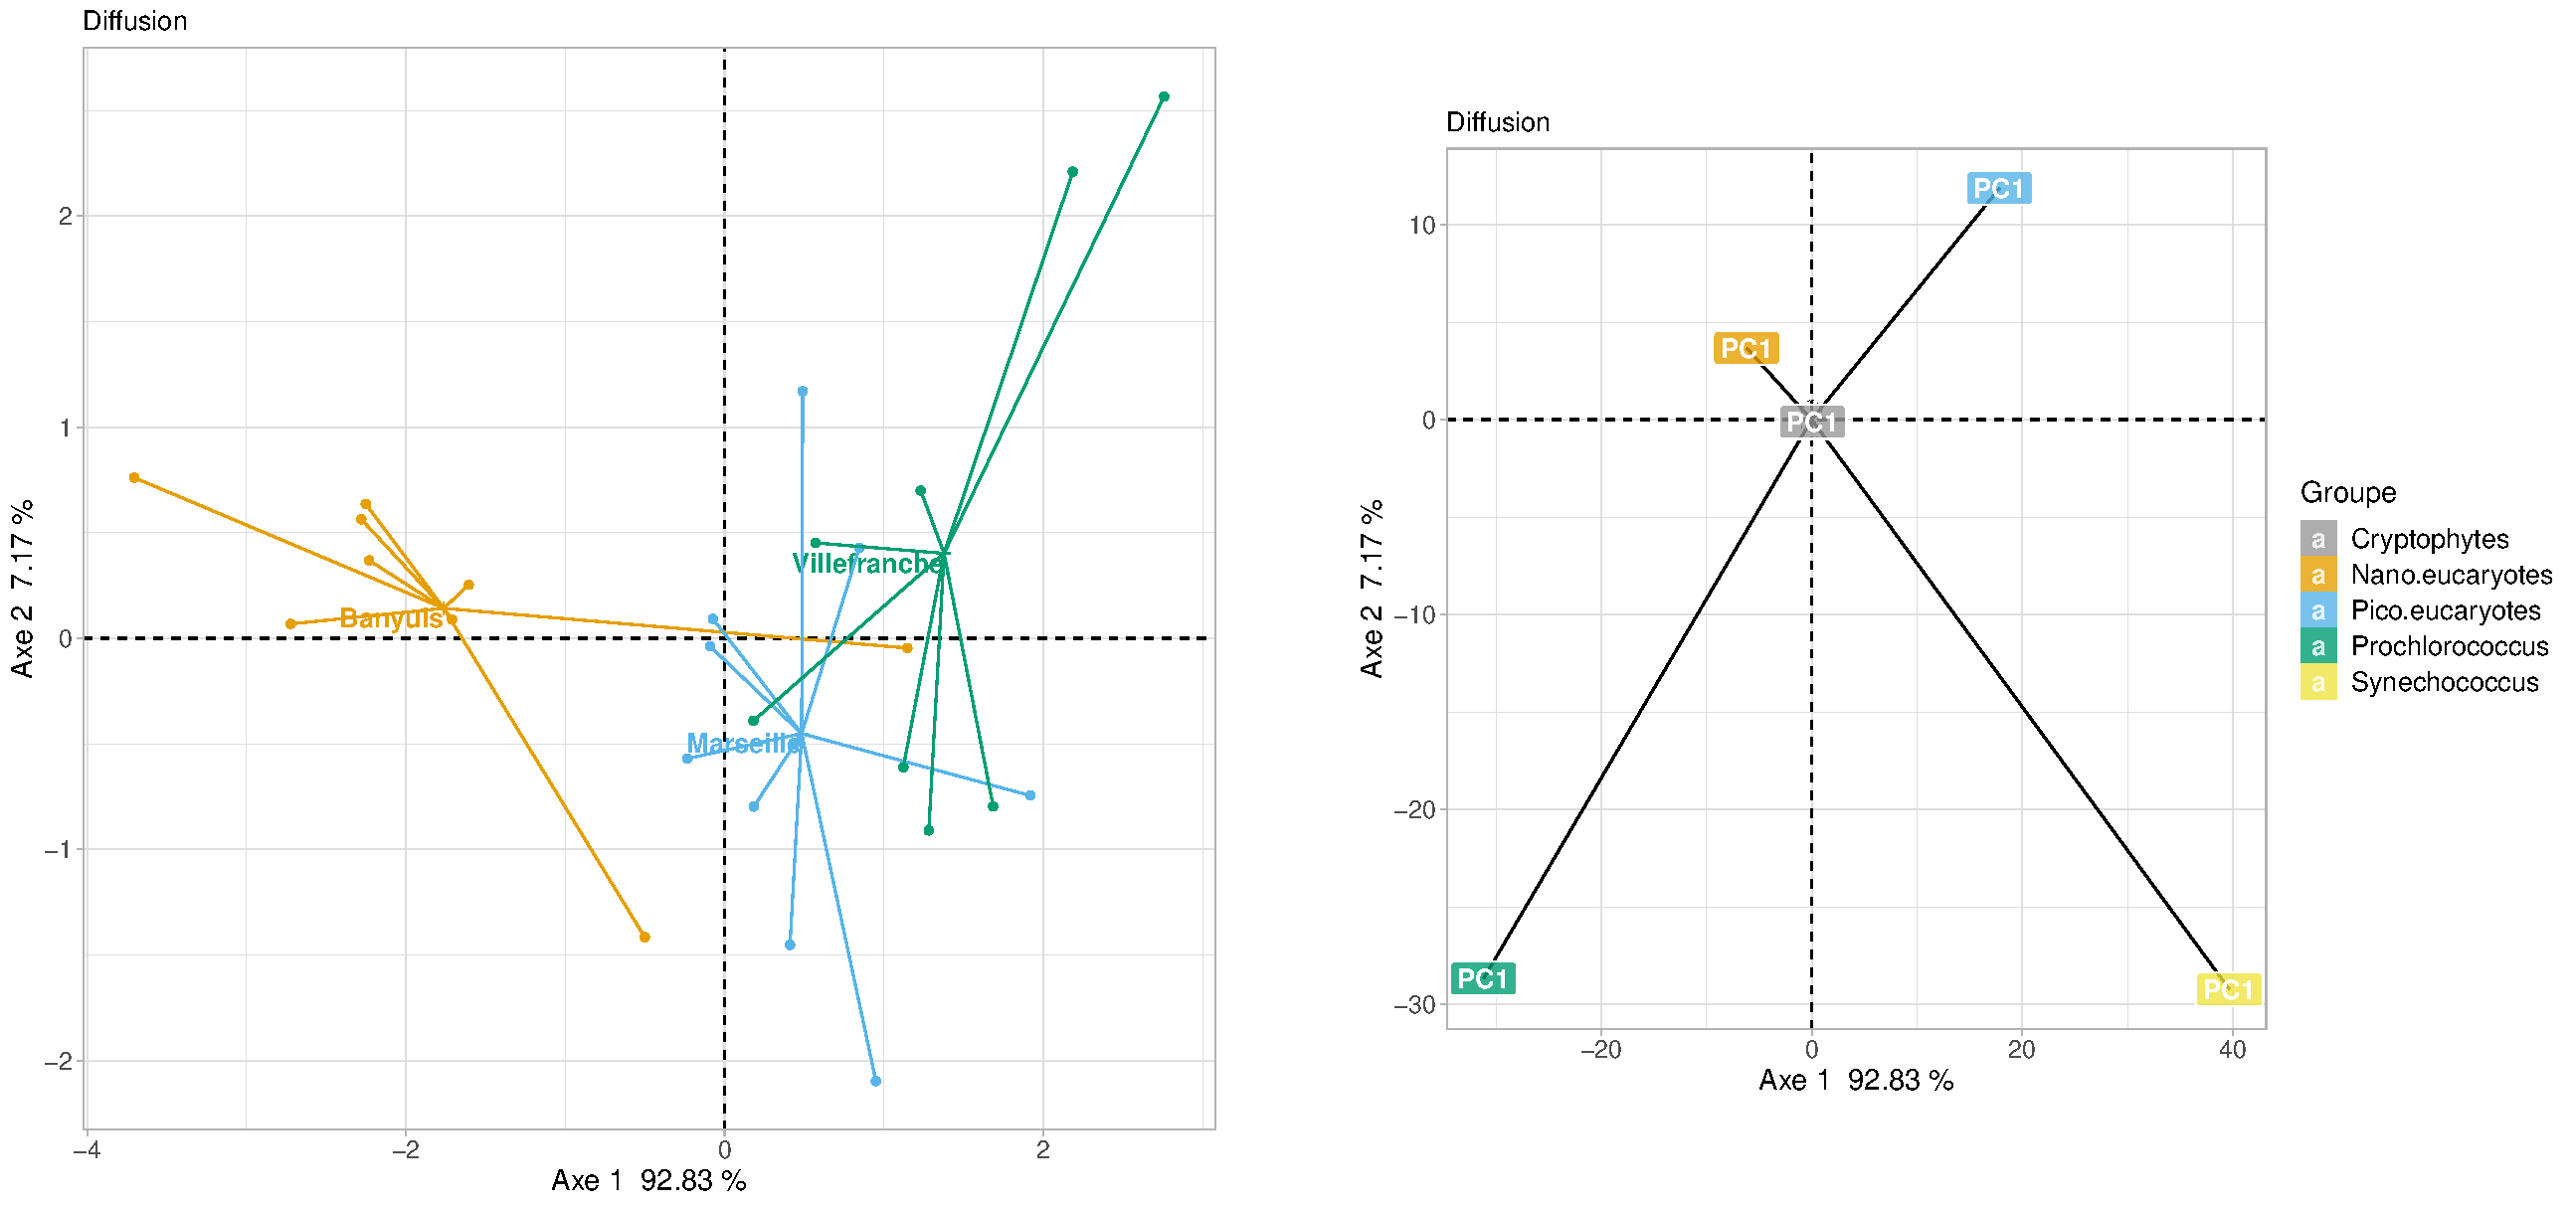
\includegraphics[width=.95\textwidth]{fig/R224_FDA_diff.pdf}
\caption{(gauche) Graphique des individus et (droite) graphique des corrélations des variables de l'AFD des unités annuelles de diffusion lumineuse des groupes de phytoplancton pour les trois stations SOMLIT méditerranéennes.}
\label{afd_diff}
\end{figure}

\subsubsection{Nutriments}

Enfin, nous cherchons à distinguer les sites par rapport à leur richesse en différents nutriments. 

Cette fois, au lieu d’avoir 5 groupes de phytoplancton, nous nous intéressons à 5 nutriments NH$_4$, NO$_3$, NO$_2$, PO$_4$, Si(OH)$_4$. Une ACP est réalisée pour chaque nutriment toutes stations confondues, avec leurs données de concentration. Les deux premières composantes des ACP sont présentées en Annexe B sous forme de perturbations de la moyenne. L’effet de toutes les premières composantes principales est un effet moyen où des valeurs positives impliquent une augmentation et des valeurs négatives impliquent une diminution. L’inertie des deuxièmes composantes principales des ACP est majoritairement inférieure à 15\%. Nous choisissons donc de ne pas conserver ces deuxièmes composantes principales pour l’AFD.

Nous obtenons alors un nouveau tableau d’observations. Chaque observation correspond à une année, avec une variable qualitative qui correspond au site et 5 variables quantitatives qui correspondent aux scores de la première composante principale des ACP pour chaque nutriment. 

Les résultats de l’AFD est présenté en Figure \ref{afd_nut}. Les deux axes résument bien 100\% des informations. Le premier est celui qui contribue le plus à la discrimination, à hauteur de 76,18\%. Le deuxième axe a donc une contribution de 23,82\%. Le premier axe permet une bonne discrimination du site de Villefranche des deux autres. Le deuxième axe quant à lui, discrimine bien le site de Banyuls des deux autres. La corrélation de variables montre que de fortes concentrations en nitrate et en amonium s’opposent à de fortes concentrations en phosphate et en nitrite. Le site de Banyuls est plutôt riche en nitrate et en amonium et plus pauvre en phosphate et nitrite, à l’inverse de  Villefranche. Le site de Marseille est particulièrement riche en silice, par rapport aux deux autres, mais avec des caractéristiques plus proches de Banyuls. 


\begin{figure}
\centering
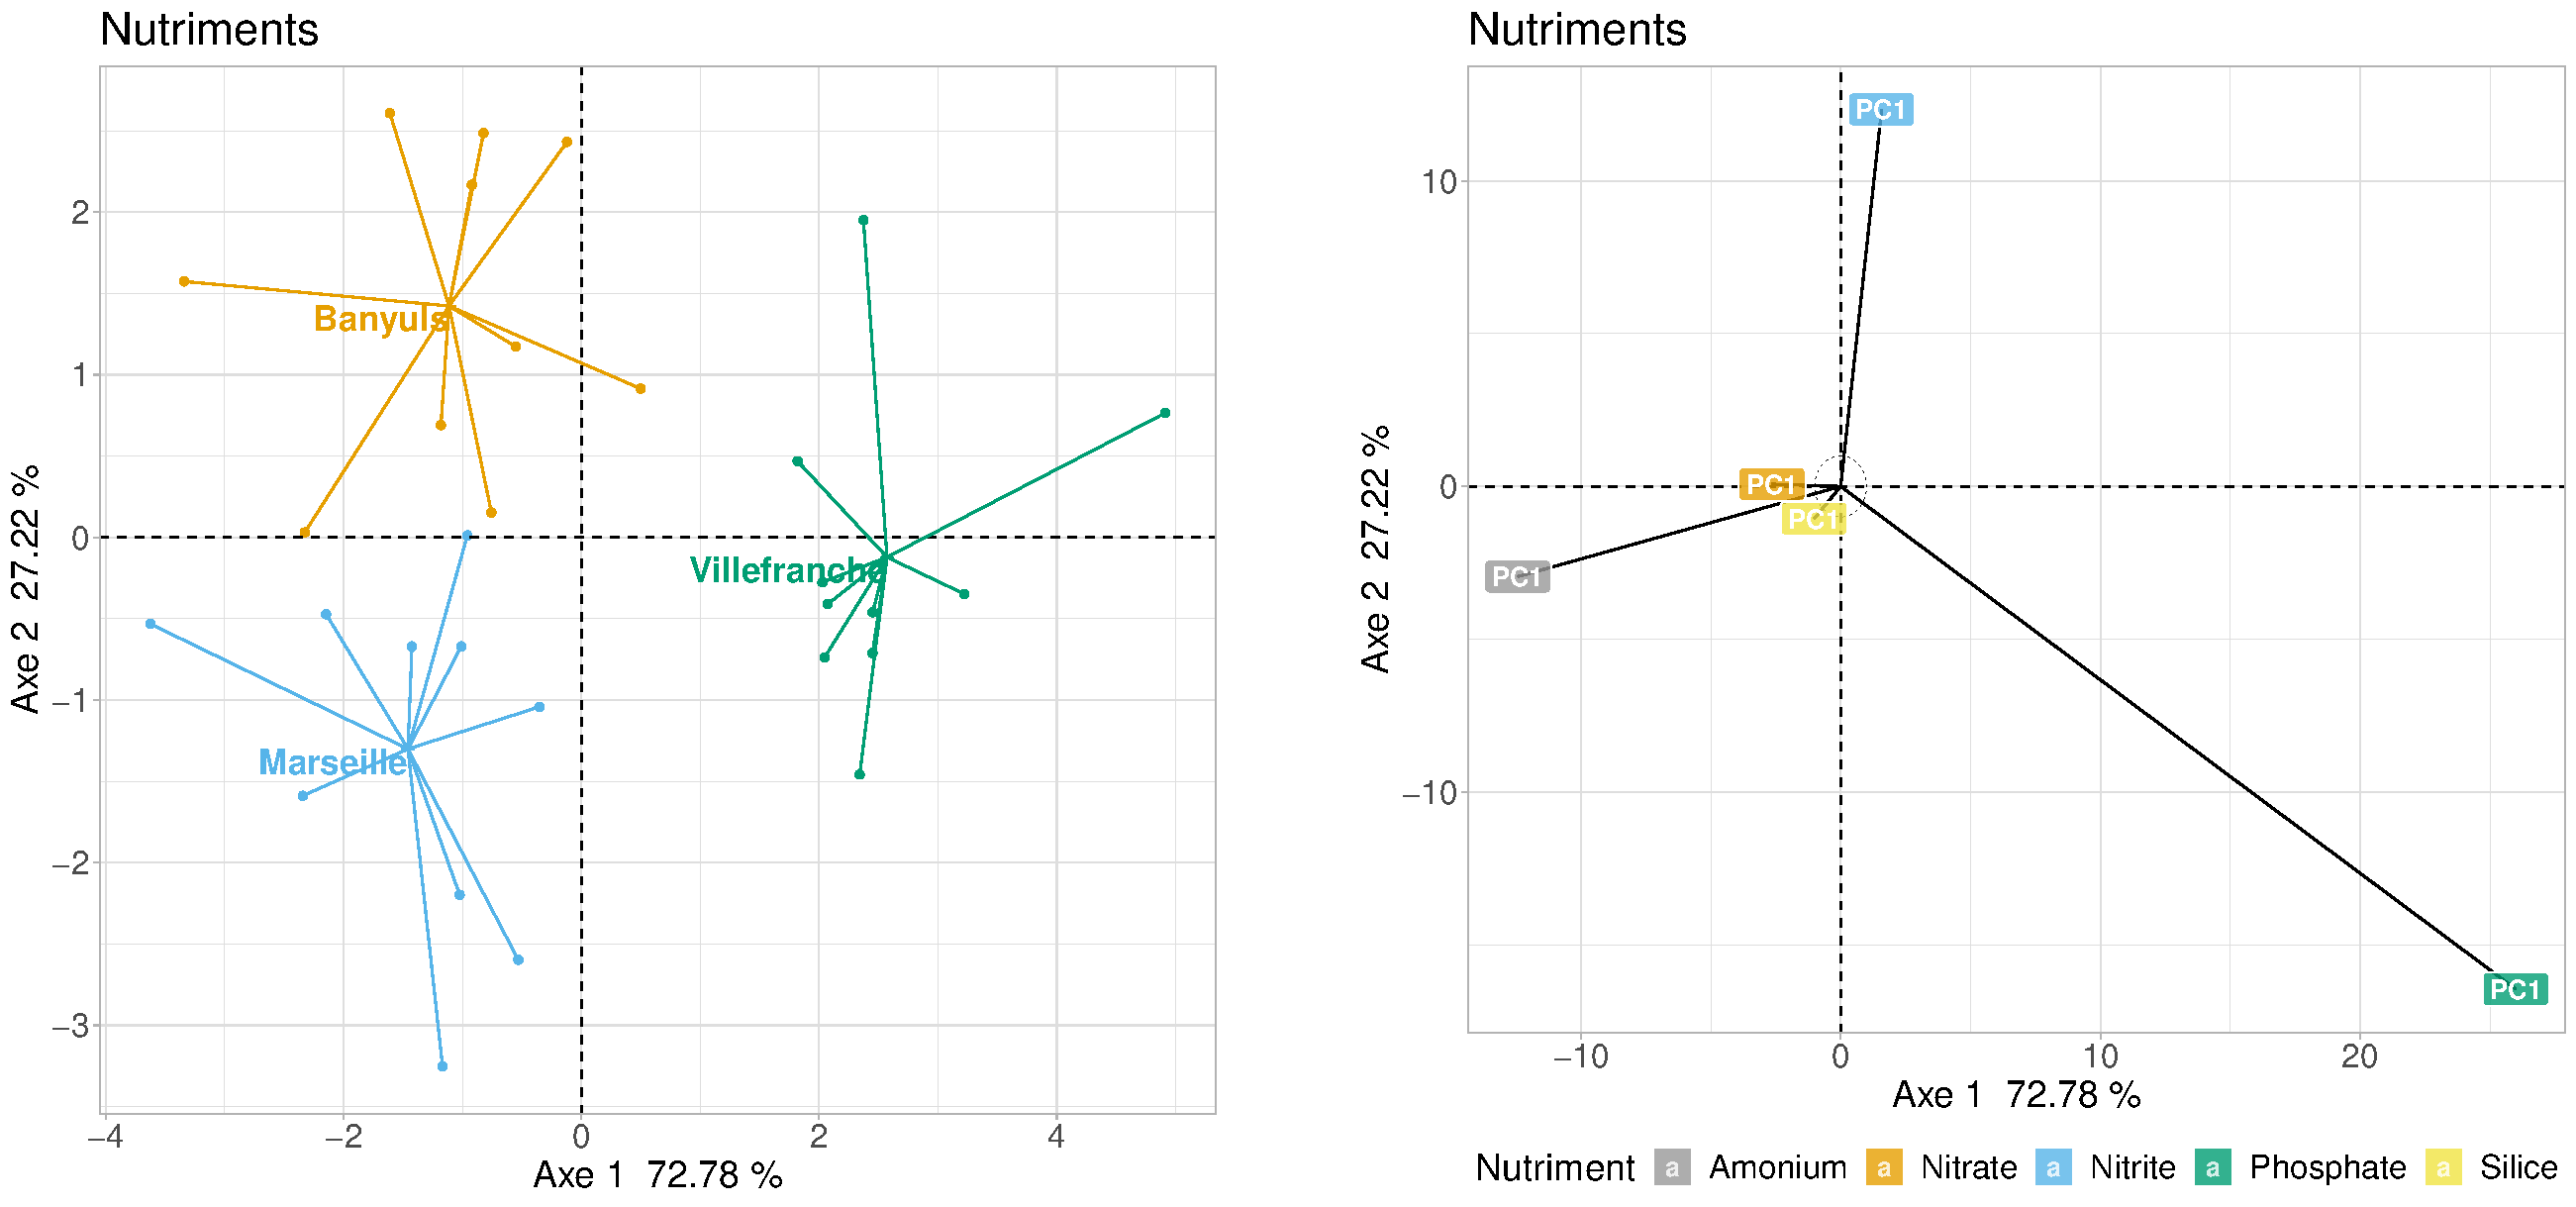
\includegraphics[width=.95\textwidth]{fig/R223_FDA_nutri.pdf}
\caption{(gauche) Graphique des individus et (droite) graphique des corrélations des variables de l'AFD des unités annuelles de concentration des nutriments pour les trois stations SOMLIT méditerranéennes.}
\label{afd_nut}
\end{figure}

\subsection{Co-variations}

Nous voulons étudier comment la structuration des communautés est influencée par les conditions environnementales et notamment la richesse du milieu. 

\subsubsection{Abondance et Nutriments}

Dans un premier temps, nous nous intéressons au lien entre l'abondance des différents groupes de phytoplancton et la concentration de chaque nutriment.   

Nous utilisons les scores des premières composantes principales des ACP sur les données d’abondance du phytoplancton et de concentrations en nutriments. Elles rendent toutes compte d’un effet moyen (Annexes A et B). Nous avons donc deux jeux de données, d’une part les données d’abondance et d’autre part les données environnementales. Chacun des jeux de données comporte 5 variables pour les 5 ACP respectives. Les individus pour chacun des tableaux sont les mêmes. Un individu correspond à une année, à un site.

L’ACC de ces deux tableaux produit les résultats présentés en Figure \ref{cca_ab}. Les deux premières corrélations canoniques pour les dimensions 1 et 2 s’élèvent respectivement à 0.853 et 0.717.  Les trois autres corrélations correspondant aux dimensions 3, 4 et 5 sont inférieures à 0.5. Sur la Figure \ref{cca_ab} seules les deux premières dimensions sont représentées. Le graphique de droite permet de comprendre les relations entres les variables. Plus elles sont proches, plus elles sont corrélées. Ce graphique met en évidence une forte corrélation entre l’abondance des  \textit{Prochlorococcus} et la concentration en phosphate. L’abondance des pico-eucaryotes semblent être plutôt corrélée à la concentration en nitrate. Le graphique des individus sépare assez bien les trois sites. Une opposition entre les sites de Villefranche et Banyuls apparaît, avec d’un côté un site avec une concentration plus importante en PO$_4$ et une abondance plus importante des \textit{Prochlorococcus} et de l’autre, un site avec une concentration plus élevée en NO$_3$ et une abondance des pico-eucaryotes plus importante. 

\begin{figure}
\centering
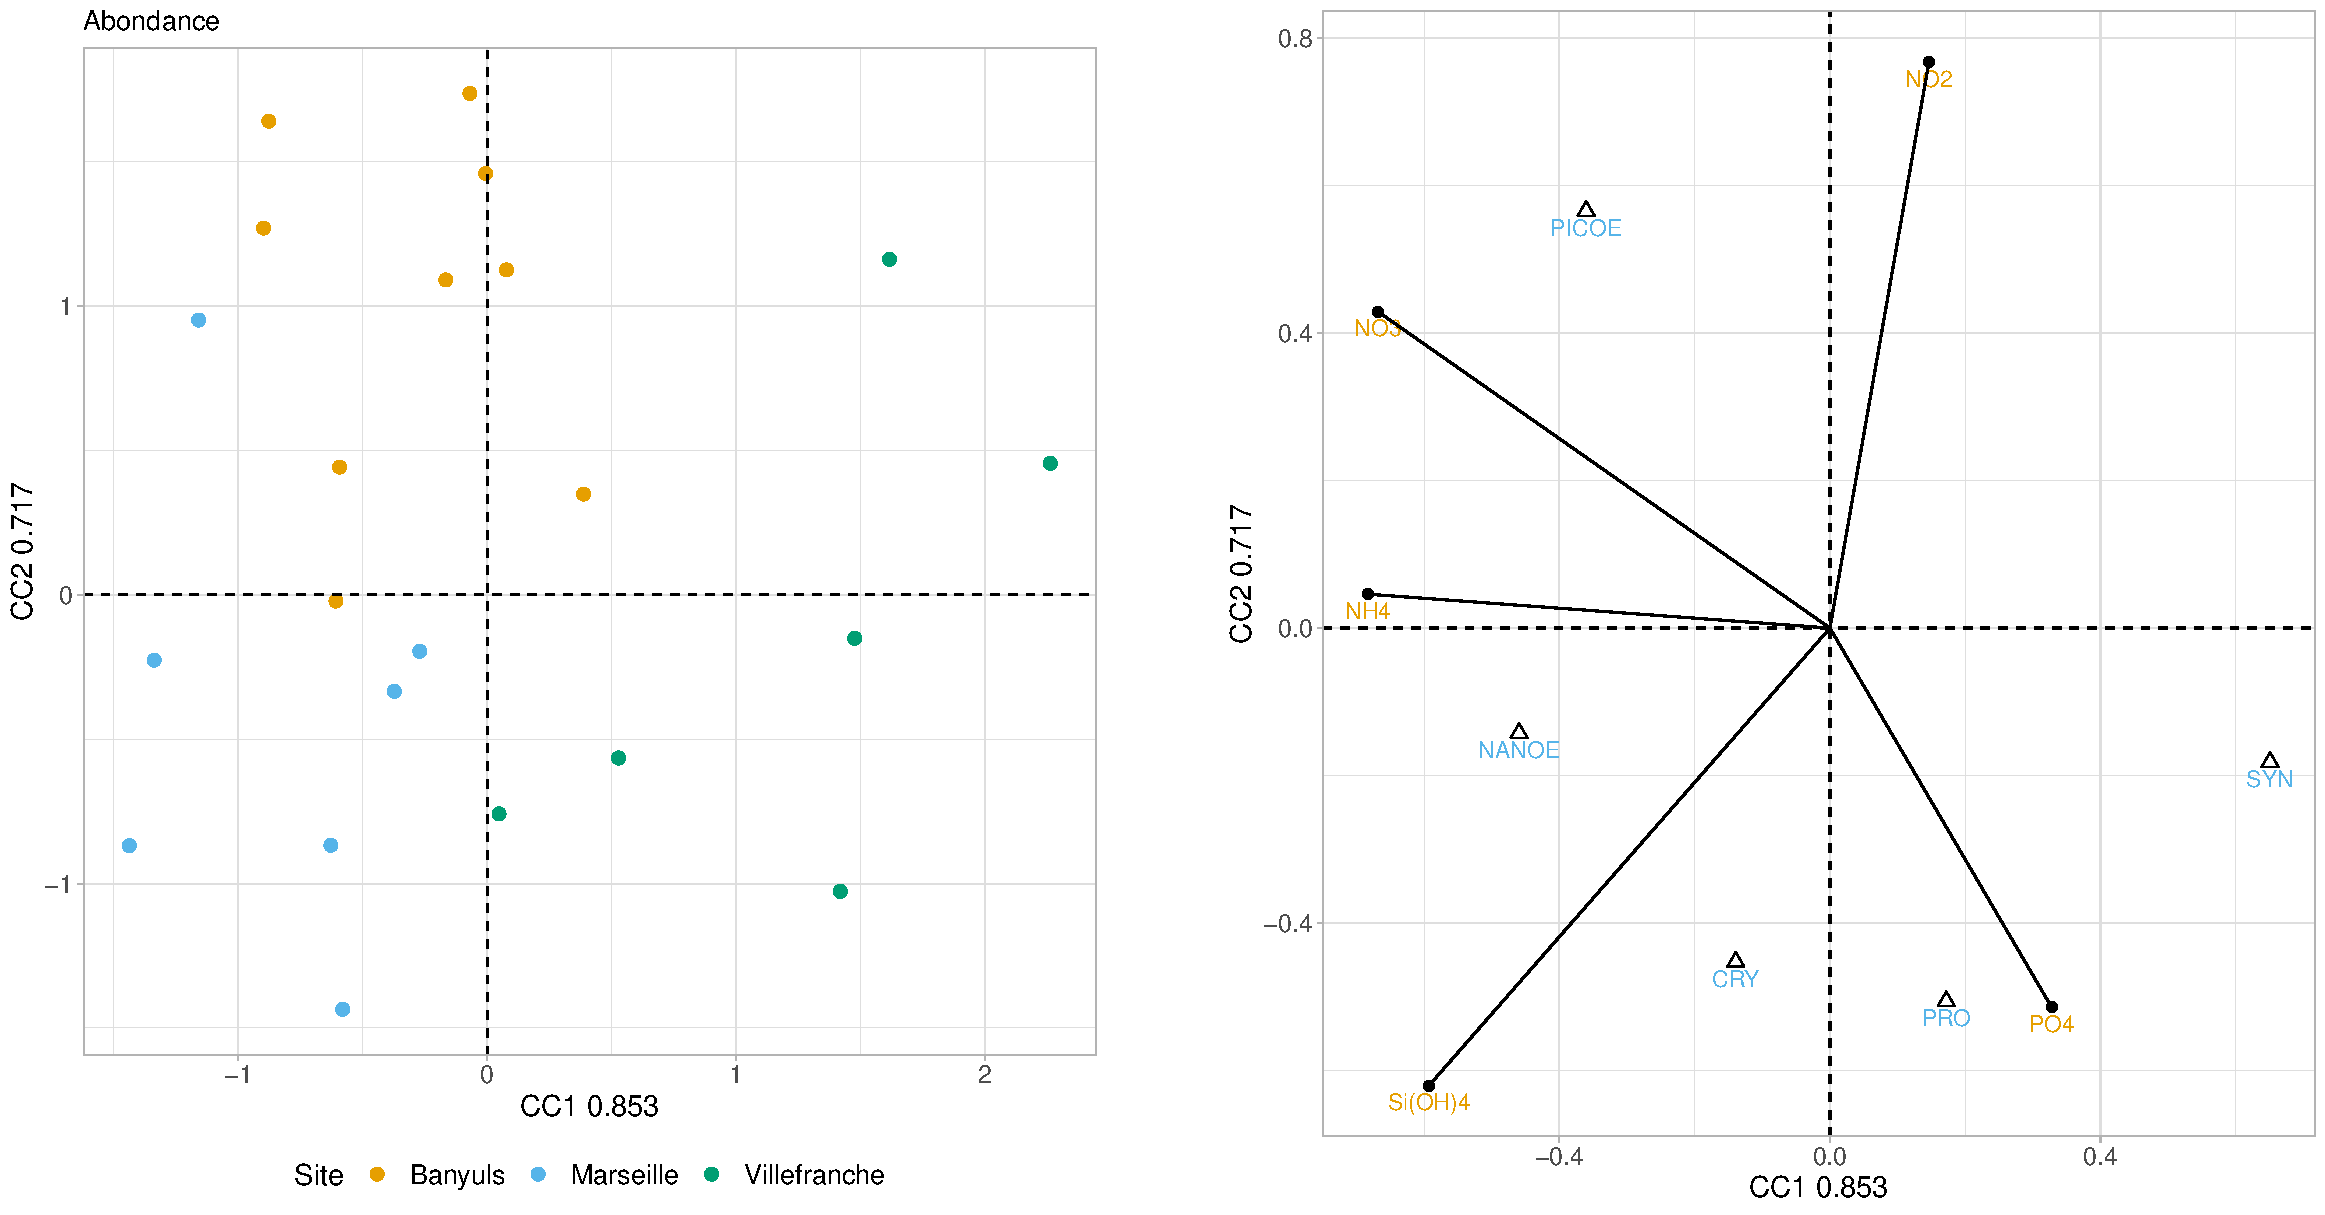
\includegraphics[width=.95\textwidth]{fig/R231_CCA_ab.pdf}
\caption{(gauche) Graphique des individus et (droite) graphique des corrélations des variables de l'ACC des unités annuelles de concentration des nutriments et de l'abondance des groupes du phytoplancton pour les trois stations SOMLIT méditerranéennes. Le premier axe correspond à la dimension 1 avec une corrélation de 0.853. Le deuxième axe correspond à la dimension 2 avec une corrélation de 0.717. Sur le graphique de droite les nutriments sont représentés par des traits et les groupes de phytoplancton (\textit{Prochlorococcus} (PRO), \textit{Synechococcus} (SYN), pico-eucaryotes (PICOE), Cryptophytes (CRY) et nano-eucaryotes (NANOE)) par des triangles.}
\label{cca_ab}
\end{figure}

\subsubsection{Diffusion lumineuse et Nutriments}

Dans un second temps, nous nous intéressons au lien entre la taille des organismes des différents groupes de phytoplancton et la concentration de chaque nutriment.   


Cette fois-ci, nous récupérons les scores de premières composantes principales des ACP sur les données de diffusion lumineuse du phytoplancton et de concentration des nutriments. Elles rendent toutes compte d’un effet moyen (Annexes B et C). Nous avons deux jeux de données, d’une part les données de diffusion SSC et d’autre part les données environnementales. Chacun des jeux de données comporte 5 variables pour les 5 ACP respectives. Les individus pour chacun des tableaux sont les mêmes. Un individu correspond à une année à un site.

L’ACC de ces deux tableaux produit les résultats présentés en Figure \ref{cca_diff}. Les deux premières corrélations canoniques pour les dimensions 1 et 2 s’élèvent respectivement à 0.71 et 0.628.  Les trois autres corrélations correspondant aux dimensions 3, 4 et 5 sont inférieures à 0.5. Sur la Figure \ref{cca_diff} seules les deux premières dimensions sont représentées. Sur le graphique des corrélations, les segments correspondant aux variables environnementales sont pratiquement orthogonaux. Cela met en évidence des relations antagonistes des variables environnementales avec la diffusion lumineuse des groupes. Les nutriments riches en azote sont opposés au phosphate.  Nous remarquons une forte corrélation entre la diffusion lumineuse des pico-eucaryotes et la concentration en phosphate. La diffusion lumineuse des Cryptophytes serait très liée à la concentration en $NH_4$. Les \textit{Synechococcus} sont très proches de l’origine. Cela signifie qu’elles ne sont pas bien représentées par ces deux dimensions. L'exploration des dimensions suivantes, permet de noter qu'elles ne sont pas mieux représentées. La SSC des \textit{Synechococcus} ne semble donc corrélée à aucun des nutriments.

\begin{figure}
\centering
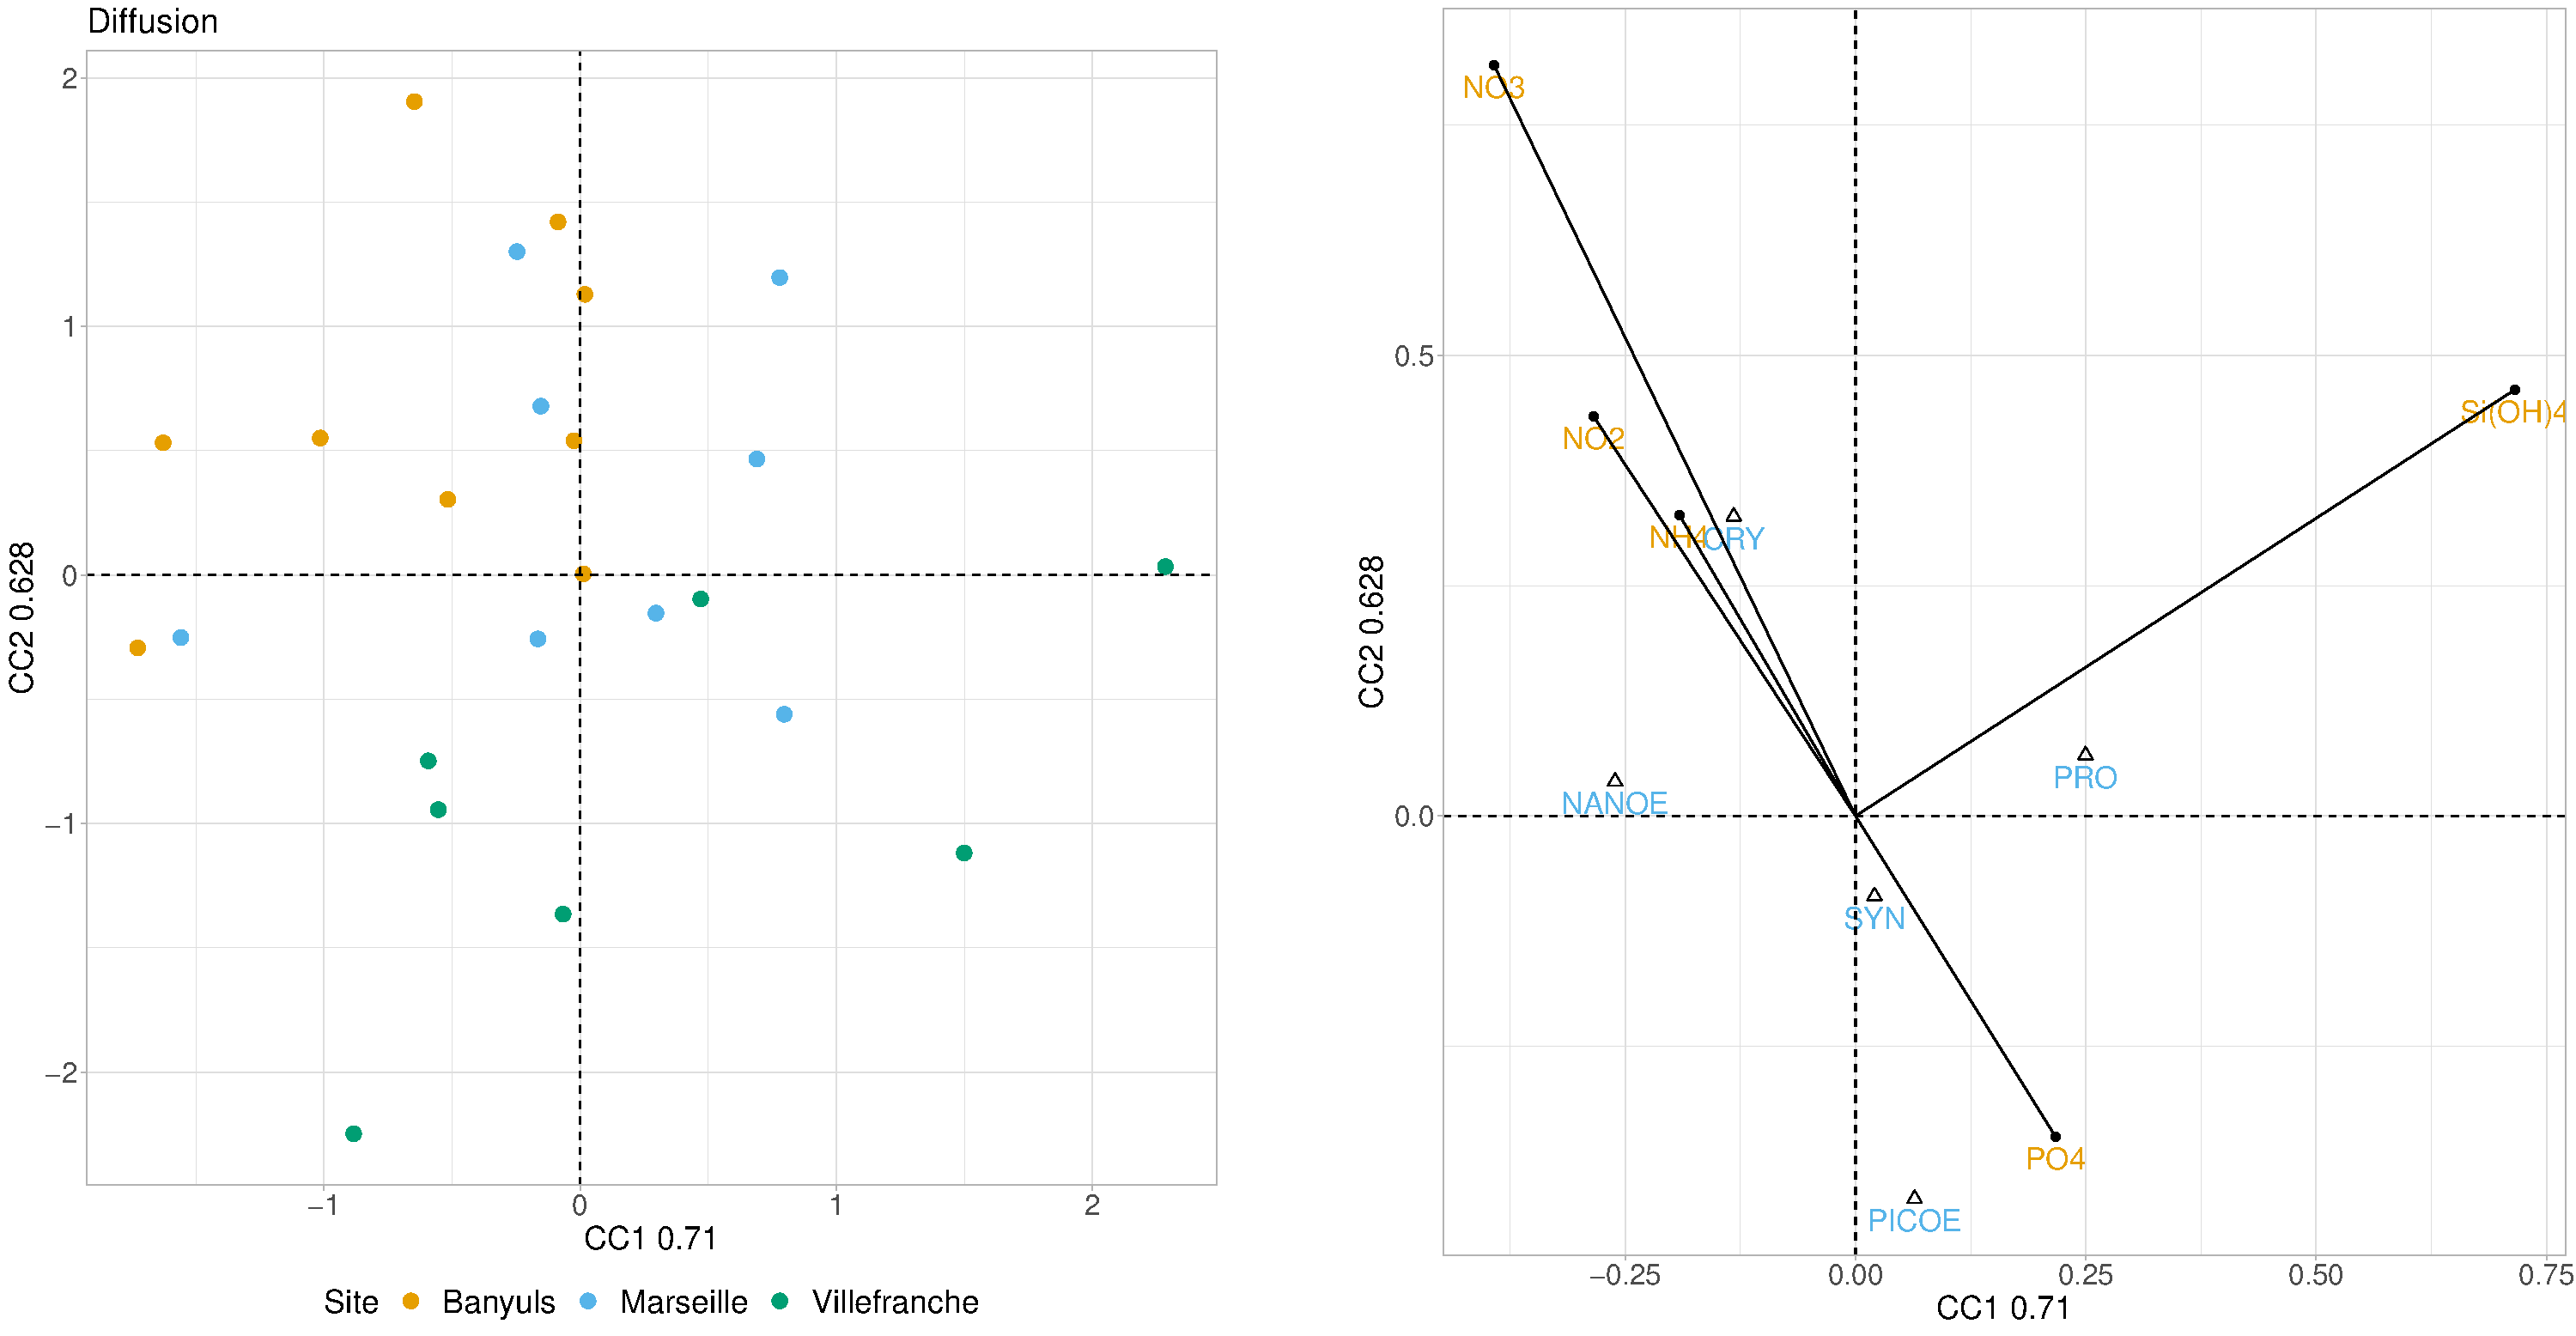
\includegraphics[width=.95\textwidth]{fig/R232_CCA_diff.pdf}
\caption{(gauche) Graphique des individus et (droite) graphique des corrélations des variables de l'ACC des unités annuelles de concentration des nutriments et de la diffusion lumineuse des groupes du phytoplancton pour les trois stations SOMLIT méditerranéennes. Le premier axe correspond à la dimension 1 avec une corrélation de 0.71. Le deuxième axe correspond à la dimension 2 avec une corrélation de 0.628. Le deuxième axe correspond à la dimension 2 avec une corrélation de 0.717. Sur le graphique de droite les nutriments sont représentés par des traits et les groupes de phytoplancton (\textit{Prochlorococcus} (PRO), \textit{Synechococcus} (SYN), pico-eucaryotes (PICOE), Cryptophytes (CRY) et nano-eucaryotes (NANOE)) par des triangles.}
\label{cca_diff}
\end{figure}

\section{Discussion}

Nous avons choisi de nous intéresser aux données collectées par le SNO SOMLIT pour les 3 stations méditerranéennes, Banyuls, Marseille et Villefranche. L’objectif de ce stage consiste à employer des méthodes d’analyses fonctionnelle et multivariée, pour (i) mettre en évidence les similitudes et dissimilitudes dans la structuration des communautés planctoniques, en tenant en compte des conditions environnementales de chaque station et (ii) caractériser la dynamique temporelle de ces communautés dans un contexte de changement global.   

Dans un contexte de réchauffement climatique, la variable environnementale qui présente un intérêt évident est la température. Les profils verticaux de température pouvant être représentés par des courbes, l’ACP fonctionnelle est un très bon outils qui nous permet de comparer la forme de tous les profils échantillonnés à Marseille de 1994 à 2021.  Cette méthode permet d’identifier les différences majeurs observées entre tous les profils. La première composante principale de l’ACP nous informe que presque 90\% des différences sont dues à une variation de la température moyenne de la colonne d’eau. % GG : Mathilde, il faudrait mentionner comment évolue la température au cours du temps, c'est à dire une tendance à l'augmentation. Ca ne me parait pas clair comme tu l'as écrit.
La deuxième composante principale nous informe que parmi les 10\% restant, 8\% des différences sont dues à la stratification de la colonne d’eau. Lorsque l’on visualise ces informations en fonction du temps, un motif saisonnier apparaît clairement pour les deux composantes principales. Les variations de la température moyenne de la colonne d’eau suivent une saisonnalité annuelle avec un refroidissement de la colonne d’eau en hiver et au printemps et un réchauffement de la colonne d’eau en été et en automne. La stratification de la colonne d’eau suit également une saisonnalité annuelle. Si la majorité de l’année la colonne d’eau est plutôt homogène, la stratification est plus importante pendant l’été. Nous mettons ainsi en évidence la formation de la thermocline saisonnière présente en Méditerranée \citep{Millot1990}. Cependant, la deuxième ACP réalisée sur les valeurs des deuxième composantes principales exprimées en fonction du temps nous permet de voir que certaines années % GG : Mathilde, précise peut-être quelles sont ces années. Ce sont les derninères??? 
, la mise en place de la thermocline est retardée par rapport à la moyenne des années observées. Ce retard est associé à une stratification plus importante de la colonne d’eau. Cette situation est de plus en plus fréquente les années les plus récentes. À l’inverse plus nous retournons dans le passé et plus nous observons la mise en place d’une thermocline moins marquée mais plus tôt dans l’année. De plus, en hiver la température en surface atteint des valeurs plus basses qu’entre 20 à 40m des profondeurs. Ces observations sont en accord avec les résultats obtenus par \citet{Rivetti2017} avec la modélisation de l’évolution de la thermocline de 1945 à 2011 à la station DYFAMED en mer Ligure.  

L’étude de la dynamique annuelle de concentration en nutriments à chaque station en utilisant les résultats des ACP couplés à une AFD permet une bonne discrimination des trois stations. Villefranche est un site particulièrement pauvre en nitrate et plus riche en phosphate en comparaison à Banyuls. Marseille semble présenter des caractéristiques plus proche de Banyuls, mais se distingue des deux sites par une concentration plus importante en silice. La mer Méditerranée est de nature oligotrophe. Cependant, à la différence de Villefranche, Marseille et Banyuls se situent dans des régions sous influence du Rhône et bénéficient donc des apports du fleuve. Le courant Nord associé aux vents, déplace les masses d’eau vers l’ouest \citep{Pairaud2011} et permet à Banyuls de bénéficier d’autant plus de ces apports. 

La dynamique annuelle des groupes de phytoplancton permet également de bien discriminer les trois sites. Ici encore, Villefranche se distingue beaucoup des autres sites. D’une part, l’abondance des pico-eucaryotes, nano-eucaryotes et Cryptophytes y est moins importante qu’à Banyuls et Marseille. D’autre part, les variations intra-annuelles des \textit{Prochlorococcus} et des nano-eucaryotes  sont celles qui permettent de distinguer le mieux Villefranche des deux autres stations.  La distinction entre Marseille est Banyuls se fait surtout par une abondance supérieure des \textit{Prochlorococcus} à Marseille. 
L’AFD réalisée avec les valeurs de diffusion lumineuse permet  de séparer uniquement Banyuls des deux autres sites. À Banyuls, les nano-eucaryotes seraient plus grosses et les \textit{Synechococcus} plus petites qu’aux deux autres sites. 

La mise en relation des variables biologiques et environnementales par l’ACC permet de comprendre en partie les résultats obtenus par les AFD. En effet, l’ACC met en évidence une corrélation positive entre l’abondance des pico-eucaryotes et la concentration en nitrate.  Si l’abondance des pico-eucaryotes présente une corrélation négative avec les phosphates, les \textit{Prochlorococcus} y sont positivement corrélés. L’abondance plus faible des pico-eucaryotes à Villefranche pourrait donc s’expliquer par la concentration plus faible en nitrate à cette station. Bien que les pico-eucoryotes soient des producteurs primaires avantagés dans un milieu mésotrophe, les \textit{Prochlorococcus} sont largement dominant dans des conditions plus oligotrophes \citep{Zubkov2000, Pan2021}. Nos résultats relatifs à l’abondance des pico-eucaryotes et des \textit{Prochlorococcus} aux trois stations, Villefranche, Marseille et Banyuls, de la plus oligotrophe à la moins oligotrophe, semblent donc pertinents. 

%GG : Mathilde, ne montrais tu pas dans les resultats une tendance à une reduction de la taille des cellules dont tu pourrais parler ici (dans le paragraphe qui suit)?
En ce qui concerne les valeurs de diffusion lumineuse, considérées comme un indicateur de la structure des cellules,  l’ACC met en relief une forte opposition des effets des nutriments azotés et du phosphate. Il semble que les Cryptophytes présentent des cellules plus grosses lorsque le milieu est plus riche en amonium ou qu’il est plus pauvre en phosphate. Et inversement pour les pico-eucaryotes. Étant donné qu’une petite taille de cellule confère un avantage lors de l’absorption des nutriments grâce à un plus grand rapport surface volume \citep{Litchman2008}, il semble logique que la taille des cellules soit positivement corrélée à la concentration en nutriments. L’affinité particulière d’un groupe à l’azote ou au phosphate pourrait être expliquée par le fait qu’un nutriment soit plus limitant que l’autre. 
Pour confirmer ou explorer plus en détails les relations mises en évidence par l’ACC, il est envisageable de comparer deux courbes représentant des variables différentes à l’aide d’une ACC fonctionnelle \citep{Ramsay1998}.      

Tous les groupes de phytoplancton n’étant pas bien représentés par l’ACC avec les variables relatives aux nutriments, une amélioration pourrait être faite en rajoutant d’autres variables environnementale avec lesquelles certains groupes présentent plus d'affinité,  telles que la température et la salinité \citep{Zubcov200}. Cela pourrait permettre notamment d’expliquer pourquoi Banyuls se distingue autant des deux autres stations en terme de taille des nano-eucaryotes et des \textit{Synechococcus}. 

L’analyses des séries temporelles d’abondance met en évidence une saisonnalité marquée pour toutes les séries. Cette saisonnalité est différente d’un groupe à l’autre mais aussi d’une station à l’autre.  Associées aux résultats des ACP sur les dynamique annuelles de l’abondance de chaque groupe de phytoplancton, les séries temporelles mettent en évidence une variation intra-annuelle évidente au sein des groupes qui se répète globalement d’une année à l’autre. Ces variations sont cohérentes avec les précédentes études sur les variations saisonnières du phytoplancton en Méditerranée \citep{Ribera2004, Bosc2004}. L’existence de variations intra-annuelle entre différents groupes de phytoplancton est bien référencée et peut être due aux affinités des groupes pour différentes conditions de température, d’éclairement, de stratification et de disponibilités en nutriments, qui suivent des cycles saisonniers \citep{Levasseur1984, Zubkov2000, Romagnan2015}.  De plus, il déjà été mis en évidence que les variations intra-annuelle de la biomasse de phytoplancton sont dépendantes du système et notamment de sa nature plus ou moins oligotrophe \citep{Sommer2012}. 

Il est possible d’extraire la saisonnalité d’une série temporelle avec des méthodes de décomposition saisonnalité-tendance \citep{Cleveland1990, Dokumentov2021}. Ces méthodes ont été testées durant le stage, mais elles nécessitent d’être ajustées. Néanmoins, ce type de méthode permet de visualiser l’interaction d’un cycle saisonnier d’un groupe de phytoplancton avec un autre (Annexe D). Cela permettrait de comprendre comment les groupes se succèdent et interagissent entre eux ou avec une variable environnementale, comme par exemple la stratification de la colonne d’eau.

Les données SOMLIT, issues d’un échantillonnage bimensuel d’un grand nombre de variables, se prêtent bien aux méthodes d’analyses fonctionnelles et multivariées. Les observations sur 10 ans pour les données biologiques, et plus pour les données hydrologiques, permettent de constituer des séries d’observations suffisamment longues pour être exploitables. L’uniformisation des protocoles et de la mise en base des données pour toutes les stations SOMLIT facilite grandement les comparaisons inter-sites. Néanmoins, ce jeu de données est complexe. Il présente plusieurs dimensions : temporelle, spatiale (observations site-dépendantes) et verticale (profils CTD).  La dimension temporelle peut être étudiée en dissociant deux échelles, intra et inter-annuelles, mais aussi en les emboîtant. Une difficulté supplémentaire s’ajoute avec la faible fréquence d’échantillonnage, qui est pourtant relativement importante en comparaison aux données habituellement disponibles pour les systèmes marins. 

Si le caractère ataxonomique des données de cytométrie ne permet pas une étude de la composition spécifique, celles-ci permettent quand même une caractérisation des communautés basée sur des traits fonctionnels \citep{Litchman2008, LeQuere2005}. Pour élargir le spectre des organismes étudiés, il peut être envisagé de compléter les données de pico et nano-plancton avec les données relatives au micro-planctons du réseau PHYTOBS. 

Le fonctionnement des communautés planctoniques et l’impact que le changement global pourrait avoir sur elles, ont été plusieurs fois documentés comme étant site-dépendant \citep{Sommer2012, Domis2013}. Pour avoir une meilleure compréhension de la manière dont fonctionne les écosystèmes marins et des changements qui peuvent être attendus, il semble pertinent d’étudier le plus grand nombre de systèmes possibles. Un autre des avantages des données SOMLIT et que ces analyses peuvent être étendues au reste des stations métropolitaines.

\section{Conclusion}

text


\addcontentsline{toc}{section}{Bibliographie}
\begin{singlespace}
\bibliography{biblio}
\end{singlespace}


\newpage
\begin{appendices}

{\bfseries A. Deux premières composantes principales des ACP fonctionnelles des données d'abondance pour chaque groupe de phytoplancton des trois stations SOMLIT méditerranéennes, exprimées comme perturbation de la moyenne. Les courbes noires correspondent aux courbes moyennes. En croix grises est représenté l’effet d’une perturbation positive et en tirets orange est représenté l’effet d’une perturbation négative. }

\begin{figure}
\centering
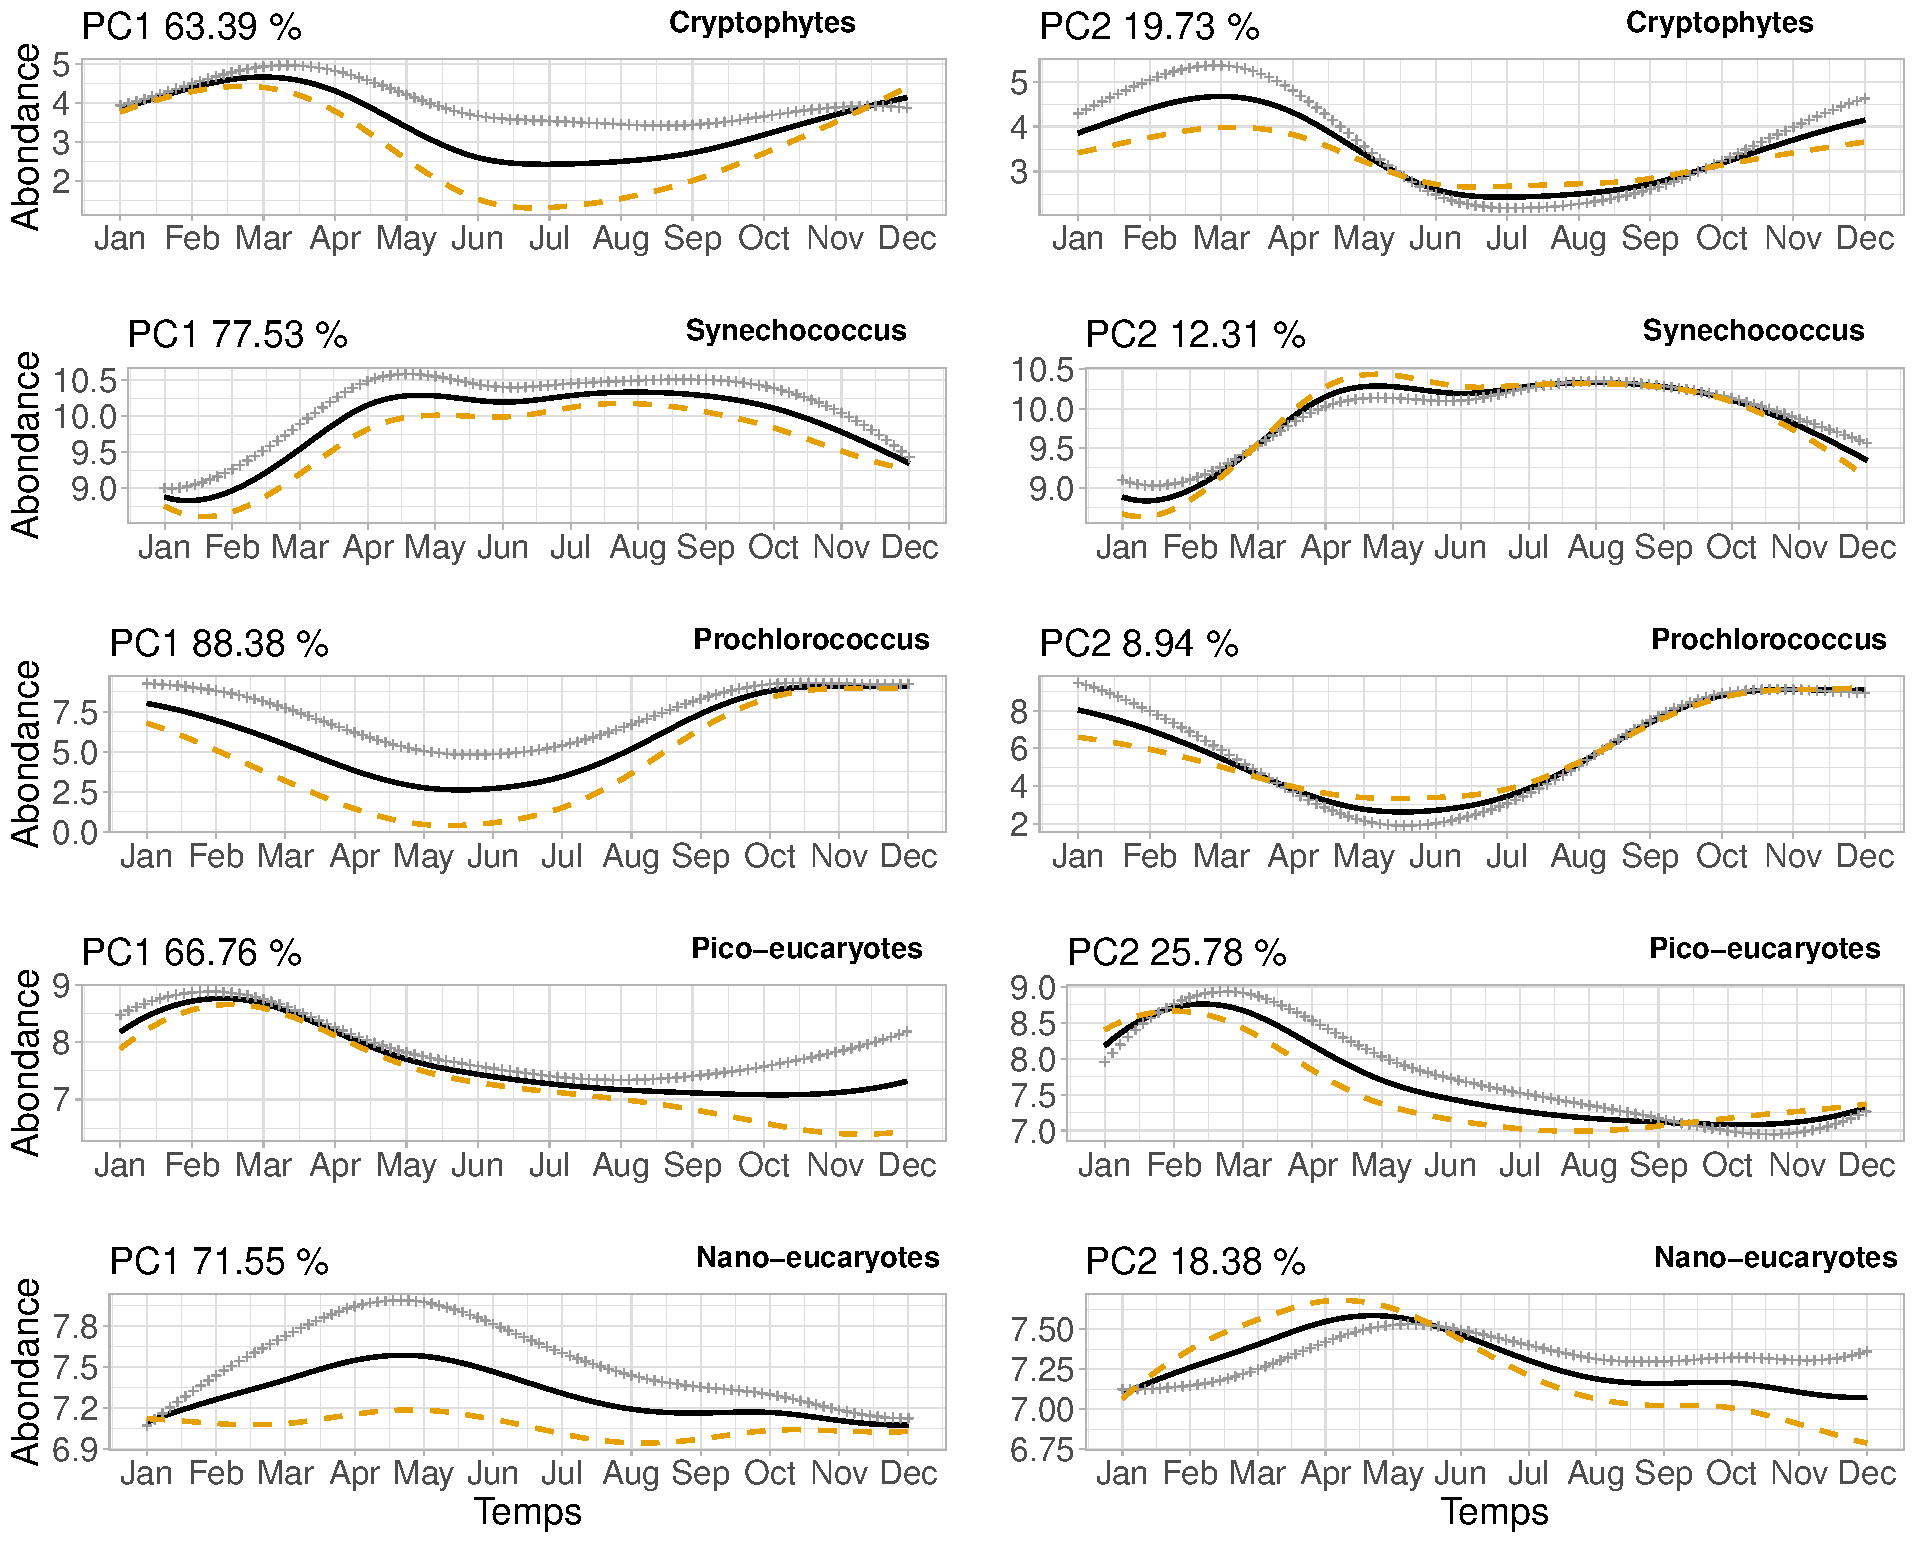
\includegraphics[width=\textwidth, height=.75\textheight]{fig/ANNEXE_fpca_ab.pdf}
\end{figure}

\newpage

{\bfseries B. Deux premières composantes principales des ACP fonctionnelles des données de concentration pour chaque nutriments aux trois stations SOMLIT méditerranéennes, exprimées comme perturbation de la moyenne. Les courbes noires correspondent aux courbes moyennes. En croix grises est représenté l’effet d’une perturbation positive et en tirets orange est représenté l’effet d’une perturbation négative. }

\begin{figure}
\centering
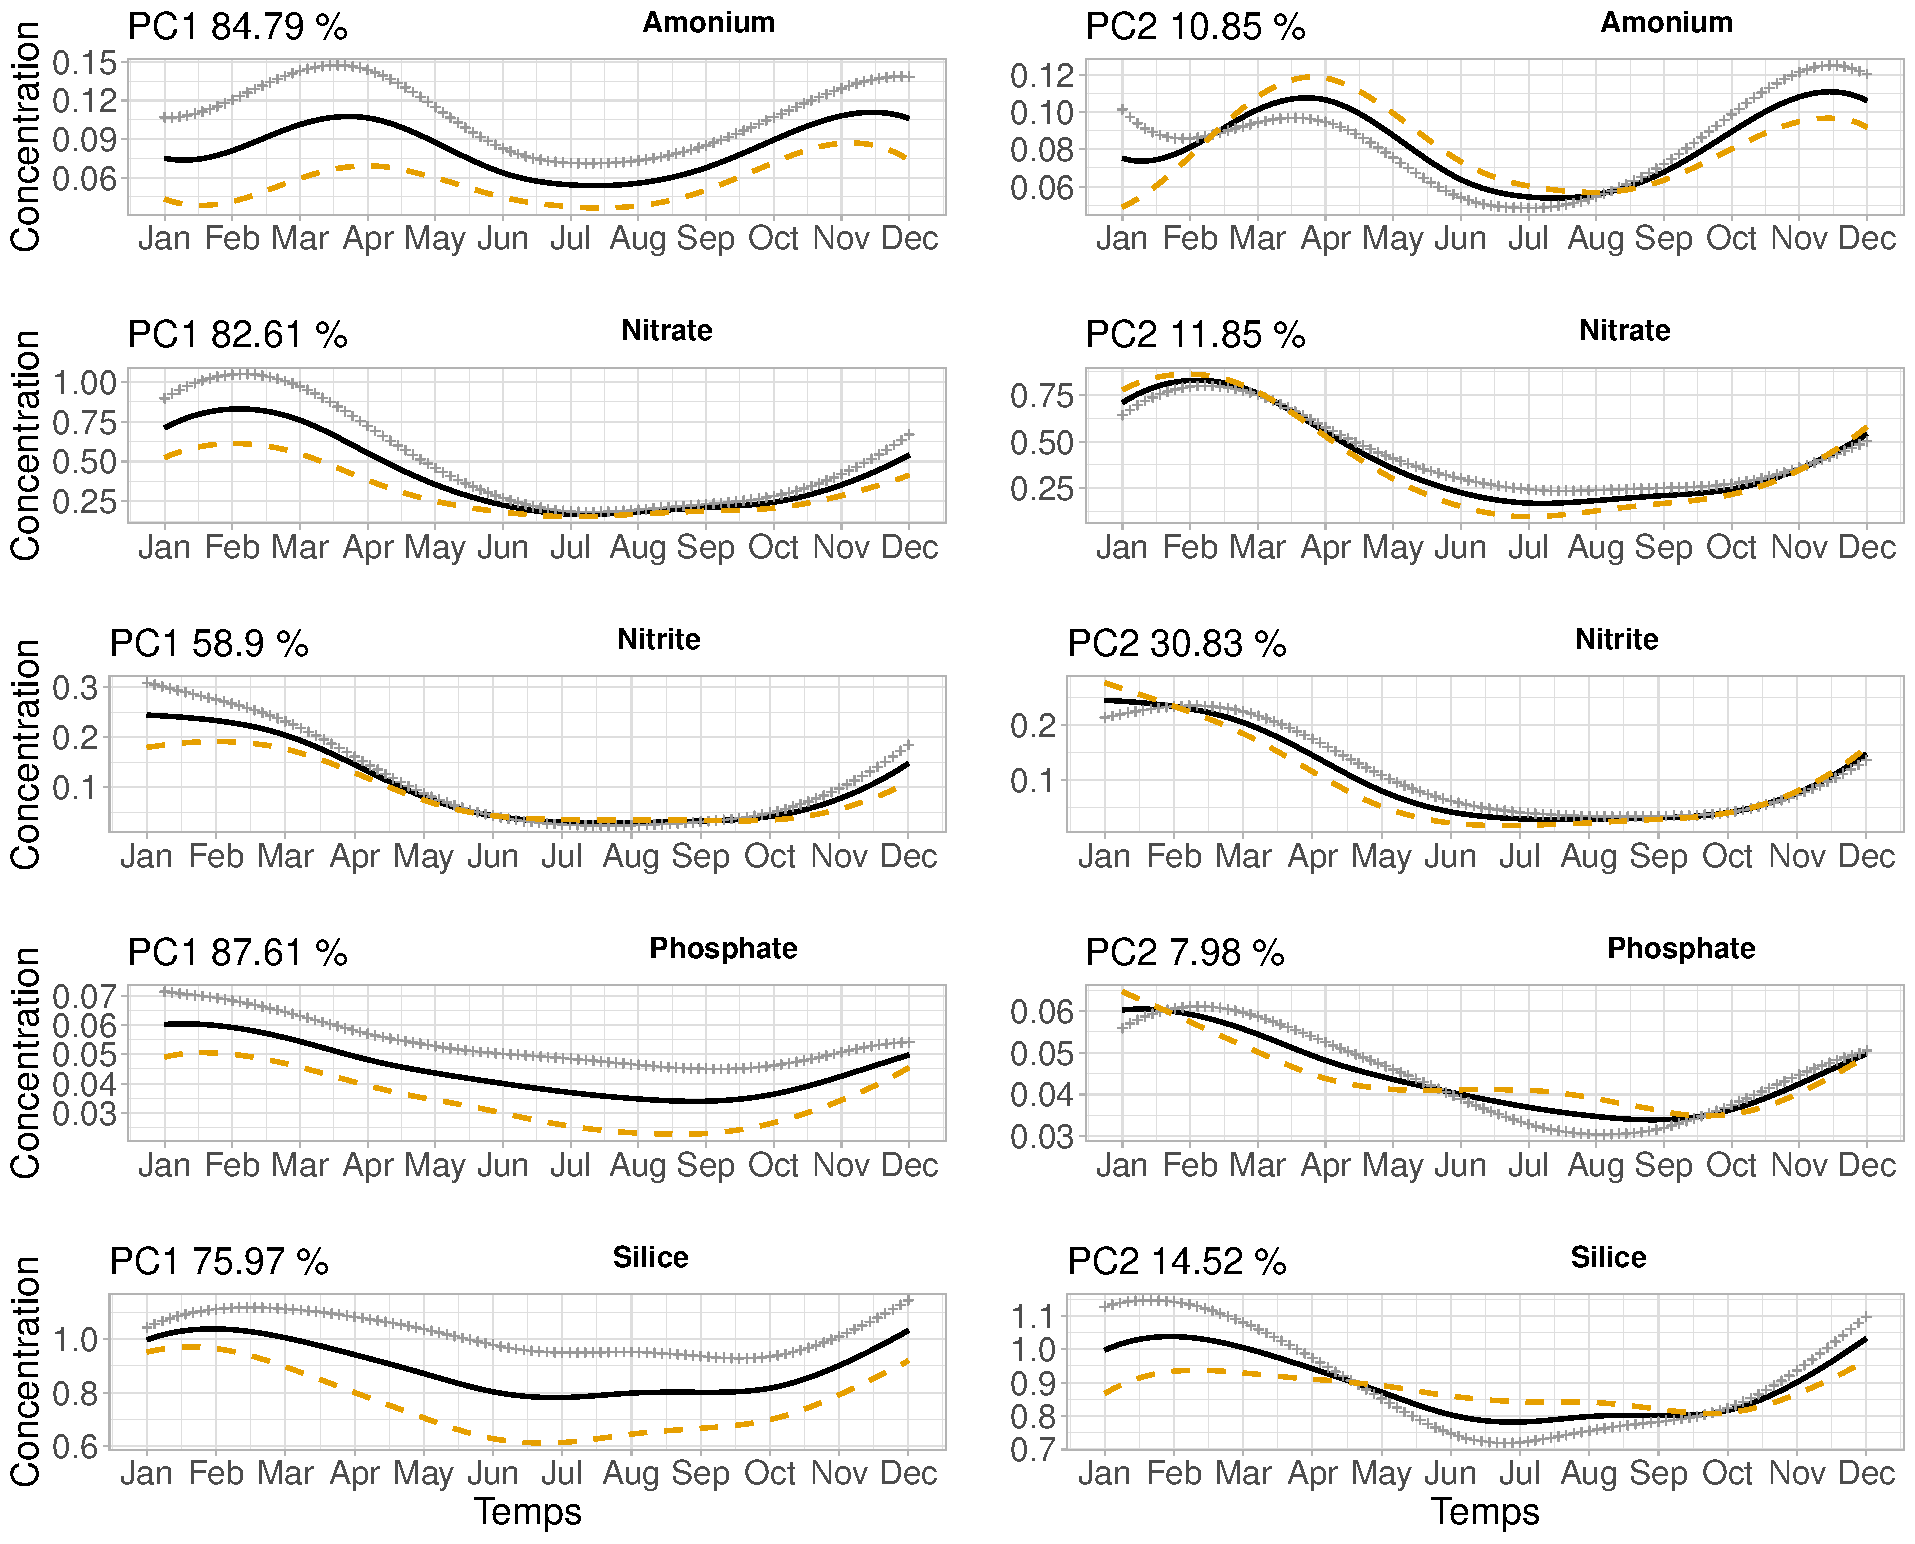
\includegraphics[width=\textwidth, height=.75\textheight]{fig/ANNEXE_fpca_nut.pdf}
\end{figure}

\newpage

{\bfseries C. Deux premières composantes principales des ACP fonctionnelles des données de diffusion lumineuse pour chaque groupe de phytoplancton des trois stations SOMLIT méditerranéennes, exprimées comme perturbation de la moyenne. Les courbes noires correspondent aux courbes moyennes. En croix grises est représenté l’effet d’une perturbation positive et en tirets orange est représenté l’effet d’une perturbation négative. }

\begin{figure}
\centering
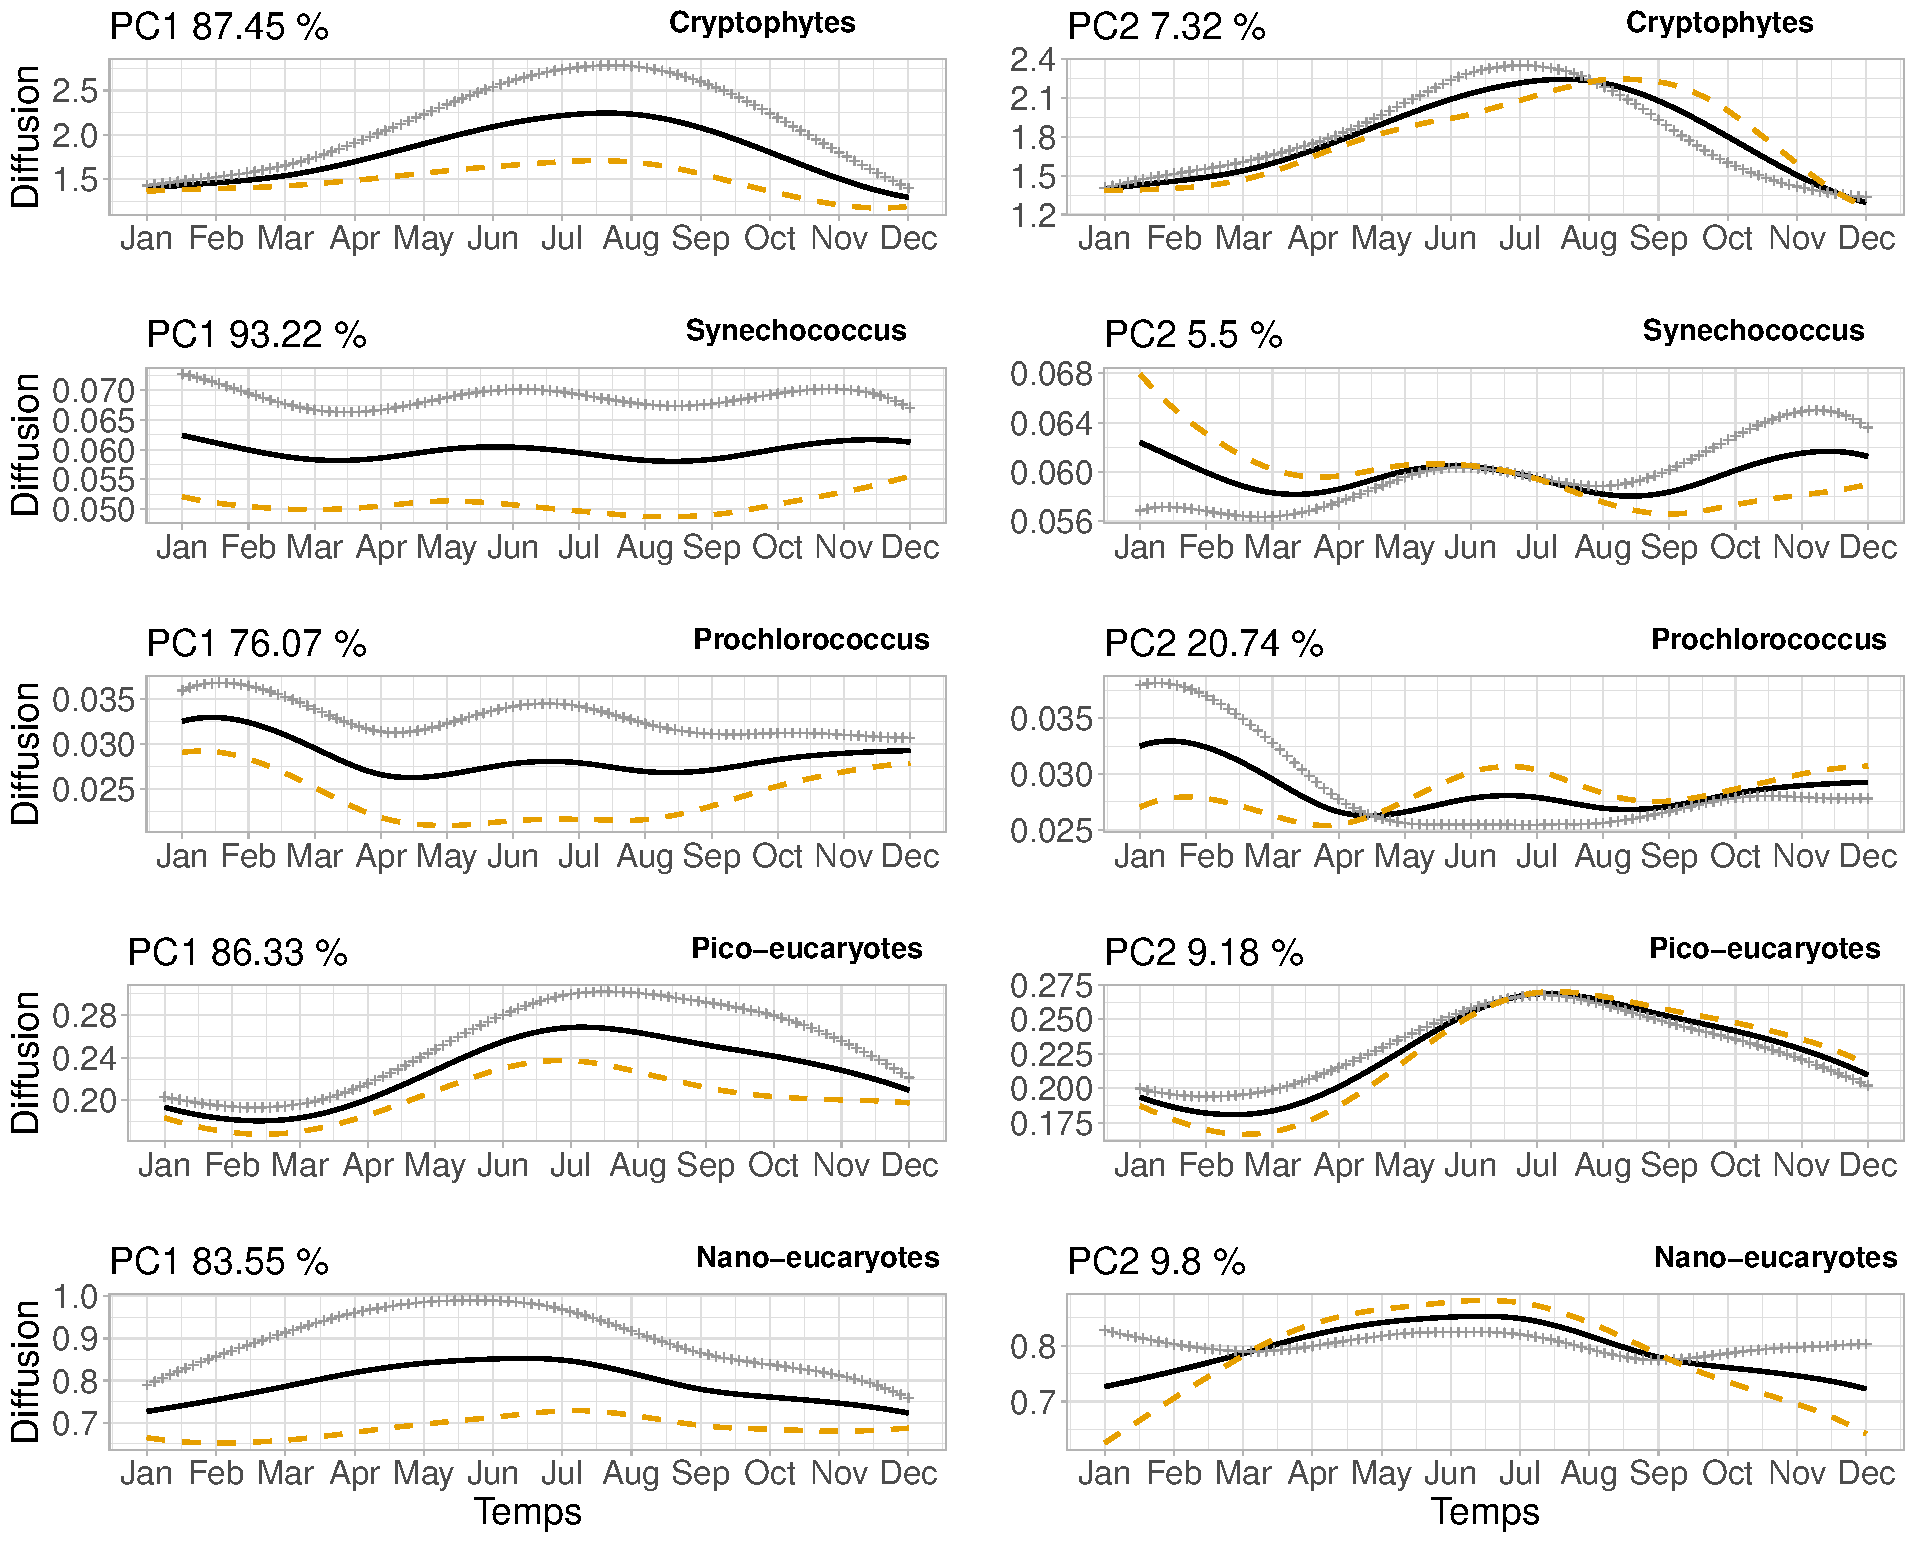
\includegraphics[width=\textwidth, height=.75\textheight]{fig/ANNEXE_fpca_diff.pdf}
\end{figure}

\newpage

\begin{landscape}
{\bfseries D. Diagrammes de phase des composantes saisonnières des séries temporelles d'abondance des groupes de phytoplancton pour les trois stations SOMLIT méditerranéennes.\\}
 \begin{figure}
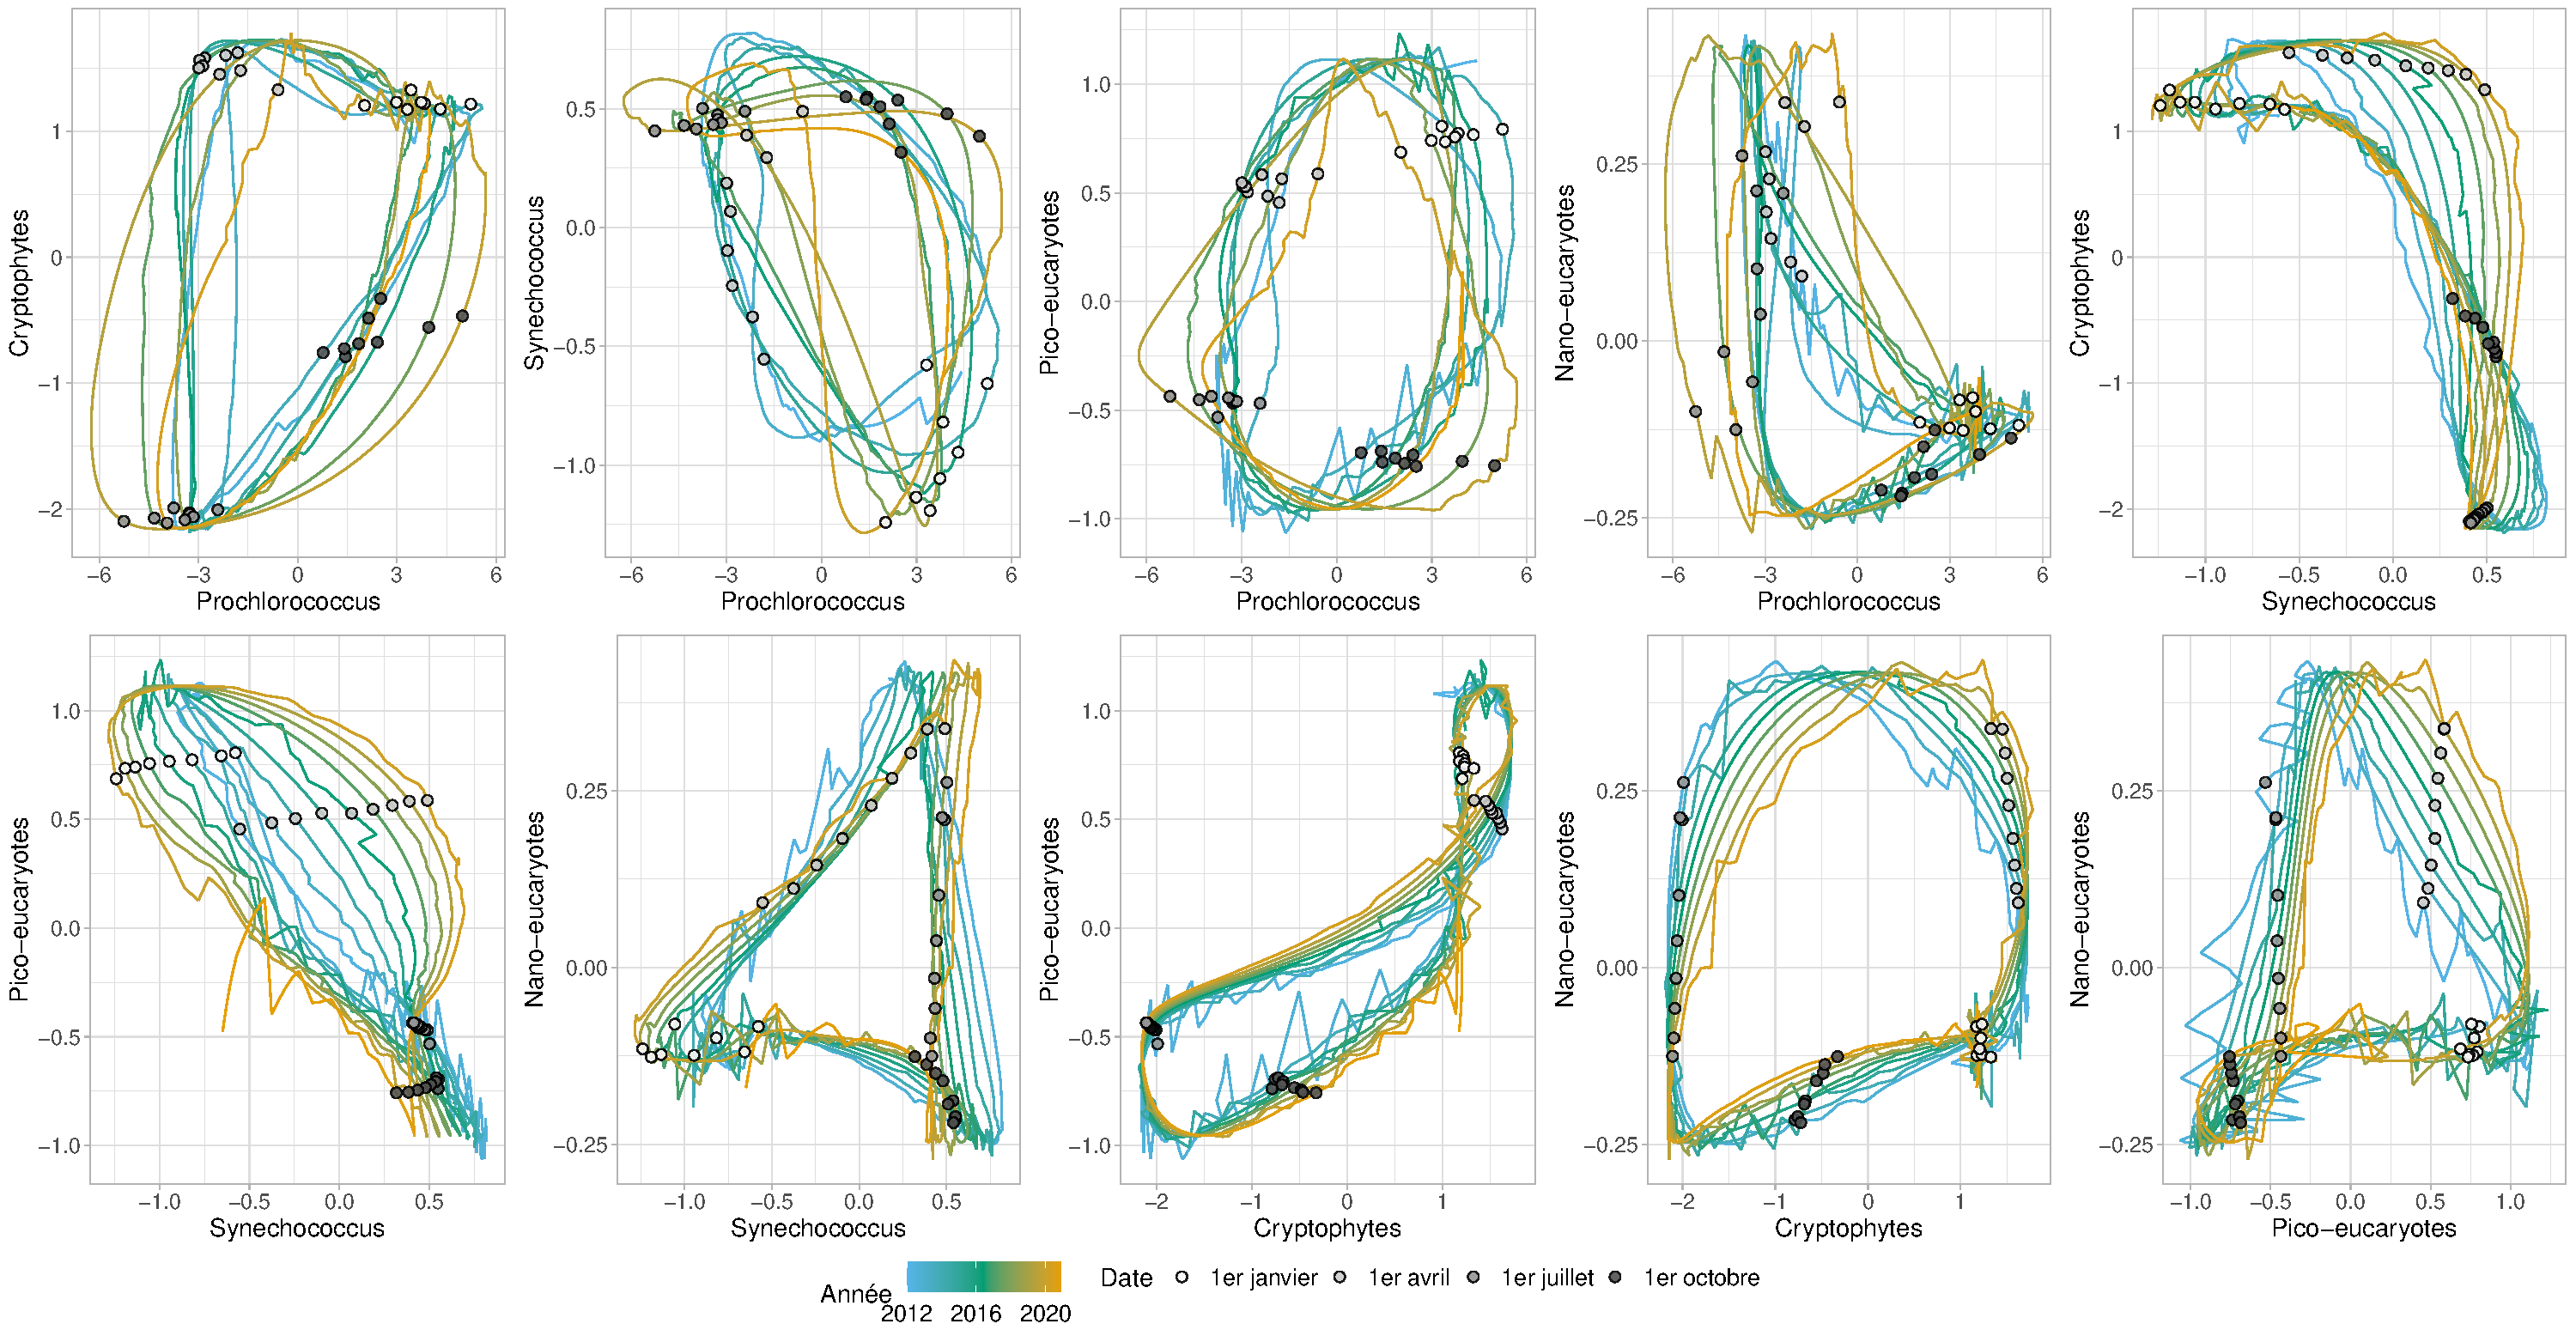
\includegraphics[height=.75\textwidth]{fig/R15_diag_phase_banyuls.pdf}
\end{figure}
\end{landscape}

\end{appendices}

\newpage 
\renewcommand{\thepage}{}

\begin{abstract}

\end{abstract}

\end{document}
